%%%%%%%%%%%%%%%%%%%%%%%%%%%%%%%%%%%%%%%%%
% Masters/Doctoral Thesis 
% LaTeX Template
% Version 1.43 (17/5/14)
%
% This template has been downloaded from:
% http://www.LaTeXTemplates.com
%
% Original authors:
% Steven Gunn 
% http://users.ecs.soton.ac.uk/srg/softwaretools/document/templates/
% and
% Sunil Patel
% http://www.sunilpatel.co.uk/thesis-template/
%
% License:
% CC BY-NC-SA 3.0 (http://creativecommons.org/licenses/by-nc-sa/3.0/)
%
% Note:
% Make sure to edit document variables in the Thesis.cls file
%
%%%%%%%%%%%%%%%%%%%%%%%%%%%%%%%%%%%%%%%%% 

%----------------------------------------------------------------------------------------
%	PACKAGES AND OTHER DOCUMENT CONFIGURATIONS
%----------------------------------------------------------------------------------------

\documentclass[11pt, oneside]{Thesis} % The default font size and one-sided printing (no margin offsets)

\graphicspath{{Pictures/}} % Specifies the directory where pictures are stored

\usepackage[comma, sort&compress]{natbib} % Use the natbib reference package - read up on this to edit the reference style; if you want text (e.g. Smith et al., 2012) for the in-text references (instead of numbers), remove 'numbers' 

%\usepackage{booktabs}
%\usepackage{array}
\usepackage{amsmath,array}
\newcolumntype{L}[1]{>{\raggedright\arraybackslash}m{#1}}
%\usepackage{apacite}
\usepackage{multirow}
\usepackage{fixltx2e}
\usepackage{enumerate}
\def\SPSB#1#2{\rlap{\textsuperscript{\textcolor{red}{#1}}}\SB{#2}}
\def\SP#1{\textsuperscript{\textcolor{black}{#1}}}
\def\SB#1{\textsubscript{\textcolor{black}{#1}}}
\newenvironment{myquote}
               {\list{}{\rightmargin   \leftmargin
                        \parsep        0in }%
                \item\relax}
               {\endlist}
\newcommand{\userquote}[2]{\begin{samepage}\begin{myquote} 
     \em{\small{#2\begin{flushright}---#1\end{flushright}}}
   \end{myquote}\end{samepage}}
\newcolumntype{x}[1]
            {>{\raggedright}p{#1}}
\newcommand{\tn}{\tabularnewline}

\hypersetup{urlcolor=blue, colorlinks=true} % Colors hyperlinks in blue - change to black if annoying
\title{\ttitle} % Defines the thesis title - don't touch this

\begin{document}
\bibpunct[, ]{(}{)}{;}{a}{,}{,} 
\frontmatter % Use roman page numbering style (i, ii, iii, iv...) for the pre-content pages

\setstretch{1.3} % Line spacing of 1.3

% Define the page headers using the FancyHdr package and set up for one-sided printing
\fancyhead{} % Clears all page headers and footers
\rhead{\thepage} % Sets the right side header to show the page number
\lhead{} % Clears the left side page header

\pagestyle{fancy} % Finally, use the "fancy" page style to implement the FancyHdr headers

\newcommand{\HRule}{\rule{\linewidth}{0.5mm}} % New command to make the lines in the title page

% PDF meta-data
\hypersetup{pdftitle={\ttitle}}
\hypersetup{pdfsubject=\subjectname}
\hypersetup{pdfauthor=\authornames}
\hypersetup{pdfkeywords=\keywordnames}

%----------------------------------------------------------------------------------------
%	TITLE PAGE
%----------------------------------------------------------------------------------------

\begin{titlepage}
\begin{center}

\textsc{\LARGE \univname}\\[1.5cm] % University name
\textsc{\Large Doctoral Thesis}\\[0.5cm] % Thesis type

\HRule \\[0.5cm] % Horizontal line
{\huge \bfseries \ttitle}\\[0.4cm] % Thesis title
\HRule \\[1.5cm] % Horizontal line

\begin{minipage}{0.4\textwidth}
\begin{flushleft} \large
\emph{Author:}\\
{\authornames} % Author name - remove the \href bracket to remove the link
\end{flushleft}
\end{minipage}
\begin{minipage}{0.4\textwidth}
\begin{flushright} \large
\emph{Supervisors:} \\
{\supname} % Supervisor name - remove the \href bracket to remove the link  
\end{flushright}
\end{minipage}\\[3cm]
 
\large \textit{A thesis submitted in fulfilment of the requirements\\ for the degree of \degreename}\\[0.3cm] % University requirement text
\textit{in the}\\[0.4cm]
\groupname\\\deptname\\[2cm] % Research group name and department name
 
{\large \today}\\[4cm] % Date
%\includegraphics{Logo} % University/department logo - uncomment to place it
 
\vfill
\end{center}

\end{titlepage}

%----------------------------------------------------------------------------------------
%	DECLARATION PAGE
%	Your institution may give you a different text to place here
%----------------------------------------------------------------------------------------

\Declaration{

\addtocontents{toc}{\vspace{1em}} % Add a gap in the Contents, for aesthetics

I, \authornames, declare that this thesis titled, '\ttitle' and the work presented in it are my own. I confirm that:

\begin{itemize} 
\item[\tiny{$\blacksquare$}] This work was done wholly or mainly while in candidature for a research degree at this University.
\item[\tiny{$\blacksquare$}] Where any part of this thesis has previously been submitted for a degree or any other qualification at this University or any other institution, this has been clearly stated.
\item[\tiny{$\blacksquare$}] Where I have consulted the published work of others, this is always clearly attributed.
\item[\tiny{$\blacksquare$}] Where I have quoted from the work of others, the source is always given. With the exception of such quotations, this thesis is entirely my own work.
\item[\tiny{$\blacksquare$}] I have acknowledged all main sources of help.
\item[\tiny{$\blacksquare$}] Where the thesis is based on work done by myself jointly with others, I have made clear exactly what was done by others and what I have contributed myself.\\
\end{itemize}
 
Signed:\\
\rule[1em]{25em}{0.5pt} % This prints a line for the signature
 
Date:\\
\rule[1em]{25em}{0.5pt} % This prints a line to write the date
}

\clearpage % Start a new page

%----------------------------------------------------------------------------------------
%	QUOTATION PAGE
%----------------------------------------------------------------------------------------

\pagestyle{empty} % No headers or footers for the following pages

\null\vfill % Add some space to move the quote down the page a bit

\textit{``Education is what remains after one has forgotten what one has learned in school.''}

\begin{flushright}
Albert Einstein
\end{flushright}

\vfill\vfill\vfill\vfill\vfill\vfill\null % Add some space at the bottom to position the quote just right

\clearpage % Start a new page

%----------------------------------------------------------------------------------------
%	ABSTRACT PAGE
%----------------------------------------------------------------------------------------

\addtotoc{Abstract} % Add the "Abstract" page entry to the Contents

\abstract{\addtocontents{toc}{\vspace{1em}} % Add a gap in the Contents, for aesthetics

The Thesis Abstract is written here (and usually kept to just this page). The page is kept centered vertically so can expand into the blank space above the title too\ldots
}

\clearpage % Start a new page

%----------------------------------------------------------------------------------------
%	ACKNOWLEDGEMENTS
%----------------------------------------------------------------------------------------

\setstretch{1.3} % Reset the line-spacing to 1.3 for body text (if it has changed)

\acknowledgements{\addtocontents{toc}{\vspace{1em}} % Add a gap in the Contents, for aesthetics

The acknowledgements and the people to thank go here, don't forget to include your project advisor\ldots
}
\clearpage % Start a new page

%----------------------------------------------------------------------------------------
%	LIST OF CONTENTS/FIGURES/TABLES PAGES
%----------------------------------------------------------------------------------------

\pagestyle{fancy} % The page style headers have been "empty" all this time, now use the "fancy" headers as defined before to bring them back

\lhead{\emph{Contents}} % Set the left side page header to "Contents"
\tableofcontents % Write out the Table of Contents

\lhead{\emph{List of Figures}} % Set the left side page header to "List of Figures"
\listoffigures % Write out the List of Figures

\lhead{\emph{List of Tables}} % Set the left side page header to "List of Tables"
\listoftables % Write out the List of Tables

%----------------------------------------------------------------------------------------
%	ABBREVIATIONS
%----------------------------------------------------------------------------------------

\clearpage % Start a new page

\setstretch{1.5} % Set the line spacing to 1.5, this makes the following tables easier to read

\lhead{\emph{Abbreviations}} % Set the left side page header to "Abbreviations"
\listofsymbols{ll} % Include a list of Abbreviations (a table of two columns)
{
\textbf{BBM} & \textbf{B}lack \textbf{B}erry \textbf{M}essenger \\
\textbf{BMI} & \textbf{B}ody \textbf{M}ass \textbf{I}ndex \\
\textbf{CHW} & \textbf{C}ommunity \textbf{H}ealth \textbf{W}orkets\\
\textbf{GPS} & \textbf{G}lobal \textbf{P}ositioning \textbf{S}ystem\\
\textbf{HCI} & \textbf{H}uman \textbf{C}omputer \textbf{I}nteraction\\
\textbf{ICT} & \textbf{I}nformation and \textbf{C}ommunications \textbf{T}echnology \\
\textbf{ICTD} & \textbf{I}nformation and \textbf{C}ommunications \textbf{T}echnology and \textbf{D}evelopment \\
\textbf{MMS} & \textbf{M}ultimedia \textbf{M}essaging \textbf{S}ervice \\
\textbf{PDA} & \textbf{P}ersonal \textbf{D}igital \textbf{A}ssistant \\
\textbf{PSD} & \textbf{P}ersuasive \textbf{S}ystem \textbf{D}esign \\
\textbf{SIM} & \textbf{S}ubscriber \textbf{I}dentity \textbf{M}odule \\
\textbf{SMS} & \textbf{S}hort \textbf{M}essaging \textbf{S}ervice \\
\textbf{USSD} & \textbf{U}nstructured \textbf{S}upplementary \textbf{S}ervice \textbf{D}ata \\
\textbf{URL} & \textbf{U}niform \textbf{R}esource \textbf{L}ocator\\
%\textbf{Acronym} & \textbf{W}hat (it) \textbf{S}tands \textbf{F}or \\
}

%----------------------------------------------------------------------------------------
%	PHYSICAL CONSTANTS/OTHER DEFINITIONS
%----------------------------------------------------------------------------------------

\clearpage % Start a new page

\lhead{\emph{Physical Constants}} % Set the left side page header to "Physical Constants"

\listofconstants{lrcl} % Include a list of Physical Constants (a four column table)
{
Speed of Light & $c$ & $=$ & $2.997\ 924\ 58\times10^{8}\ \mbox{ms}^{-\mbox{s}}$ (exact)\\
% Constant Name & Symbol & = & Constant Value (with units) \\
}

%----------------------------------------------------------------------------------------
%	SYMBOLS..
%----------------------------------------------------------------------------------------

\clearpage % Start a new pagesubscriber identity module,

\lhead{\emph{Symbols}} % Set the left side page header to "Symbols"

\listofnomenclature{lll} % Include a list of Symbols (a three column table)
{
$a$ & distance & m \\
$P$ & power & W (Js$^{-1}$) \\
% Symbol & Name & Unit \\

& & \\ % Gap to separate the Roman symbols from the Greek

$\omega$ & angular frequency & rads$^{-1}$ \\
% Symbol & Name & Unit \\
}

%----------------------------------------------------------------------------------------
%	DEDICATION
%----------------------------------------------------------------------------------------

\setstretch{1.3} % Return the line spacing back to 1.3

\pagestyle{empty} % Page style needs to be empty for this page

\dedicatory{This work is dedicated to my great parents, my father, Andalwisye, and my late mother, Mary for supporting me throughout my academic journey\ldots} % Dedication text

\addtocontents{toc}{\vspace{2em}} % Add a gap in the Contents, for aesthetics

%----------------------------------------------------------------------------------------
%	THESIS CONTENT - CHAPTERS
%----------------------------------------------------------------------------------------

\mainmatter % Begin numeric (1,2,3...) page numbering

\pagestyle{fancy} % Return the page headers back to the "fancy" style

% Include the chapters of the thesis as separate files from the Chapters folder
% Uncomment the lines as you write the chapters
% Chapter 1

\chapter{Introduction} % Main chapter title

\label{introductionchapter} % For referencing the chapter elsewhere, use \ref{Chapter1} 

\lhead{Chapter 1. \emph{Introduction}} % This is for the header on each page - perhaps a shortened title

%----------------------------------------------------------------------------------------
\section{Background}
Obesity and overweight are currently global health concerns. A systematic review by~\cite{guh2009incidence} concluded that both overweight and obesity are associated with increased incidence of multiple co-morbidities including type 2 diabetes, cancer and cardiovascular diseases (CVD). The number of people who are considered to be either overweight or obese stands to an approximation of  1.3 billion people~\citep{steyn2006chronic}. A survey by~\cite{abegunde:theburden} which included a total of 23 low-income and middle-income countries had projected a loss US\$84 billion of economic production in between 2006 and 2015 from heart disease, stroke, and diabetes alone in the absence of any significant measures put in place to intervene.

Co-morbidities that are associated with obesity are likely to inundate health care systems~\citep{pollak2010s}. At the moment health-care systems have failed to optimally treat chronic conditions such as diabetes due to lack of time to continuously provide  patient  care which is essential in management of chronic conditions~\citep{quinn2008welldoc}. Resources are insufficient to deal with an overwhelming increase in number of patients; hence there has been suggestions emphasizing on moving part of the care to the hands of patients~\citep{aarsand2012mobile}. This need calls for innovative and citizen-centric  interventions to foster lifestyle changes in order to, both prevent or delay onset of chronic conditions in poulations and also supporting of patients in self-management of a chronic conditions in order to reduce the burden on healthcare systems~\citep{korhonen2010personal,aarsand2012mobile,higgins2016smartphone}. There has been a growing number of initiatives by both commercial and research communities in development of wearable sensors and mobile applications that can nudge individuals to eat healthy and increase their level of physical activity~\citep{chen2014healthytogether}. Citizen centric interventions are now possible due to the current advancements in hardware and software technologies which have facilitated creation of opportunities for automation of health self-management processes~\citep{arsand:mobile}. 

One interesting development trend in both academia and industry is the use of mobiles in health. The mobiles have become an effective way for ``just-in time'' delivery of interventions that target psychological processes~\citep{hsu2014persuasive}. These devices are currently omnipresent and people carry them most of the time~\citep{mattila2008mobile}; hence their presence brings a ``kairo factor'' in delivery of interventions that target both health promotion ~\citep{pollak2010s} and persuasion~\citep{hsu2014persuasive}. Smartphone based applications have been rapidly gaining popularity as effective tools to support delivery of personalized health information~\citep{handel2011mhealth}. One of the prevalent adoption of mobile health apps is their use in self-monitoring to augment \emph{cognitive behaviour therapy} - treatment of behaviour in clinical settings~\citep{mattila2008mobile,medynskiy2010salud}. These apps facilitate data collection of one's health parameters through inbuilt tools such as GPS, accelerometer (body activity sensor), etc; hence present an innovative way of monitoring and improving both health and fitness~\citep{higgins2016smartphone}. In order for such tools to support changes in health behaviour and promotion of healthy lifestyle, theory based strategies such gamification (for enhancement of motivation), enabling self-reflection through goal setting and feedback (for improvement of self-efficacy), and SMS reminders are often applied~\citep{consolvo2009goal,cole2010text,hamari2014persuasive,hamari2014does,higgins2016smartphone}. However, such tools have limitations if there were to be utilized in specific contexts. The basis of the research problem for this study was on a limitation that is related to developing world context but can as well scale to a context of developed world. The research problem is as reported below.
\section{Statement of the Problem}
A review by~\cite{higgins2016smartphone} presented evidence that self-monitoring apps can help patients reach their health and fitness goals. Also these apps can support individuals who are not patients to become aware of their behaviours which is an important step towards taking actions that are necessary in living a healthily lifestyle. However, such apps have limitations as they don't support specific interaction models that accommodate sharing of devices and indirect usage. Such mode of interaction are prevalent and relevant in the context of developing world ; hence self-monitoring applications are designed for direct use may not replicate well to some populations of users~\citep{kaplan2006can,sambasivan2010}, especially the ones that face barriers of direct access to user interfaces or technology~\citep{kumar2015mobile}. Self-monitoring apps usually have motivational affordances for usage but such incentives have been designed only for the direct user as are not supported in a situation of where you have at least two layers of users that consists of an intermediary user who acts as a bridge for an indirect user who is a beneficiary of information in a self-monitoring app. Such scenario of intermediated technology is shown on Figure \ref{figure:directVSinterm}  and  it has profoundly been explained by~\cite{sambasivan2010} in the perspective of activity theory\citep{kaptelinin1997activity}, of where in direct interaction a computing device or system is an object with affordance of an activity of which an end user can act on, while in intermediated interaction there is an addition layer of human interface (intermediary user) responsible for translating intents of a beneficiary user into an an carrying out activities to a computing device or system.
\begin{figure}[htbp]
  \centering
    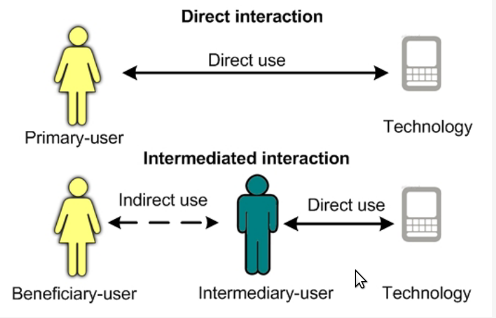
\includegraphics[width=0.6\textwidth]{Figures/intermediated.png}
    \rule{35em}{0.5pt}
  \caption{Direct and intermediated interactions~\citep{sambasivan2010}.}
  \label{figure:directVSinterm}
\end{figure}

This research explored of how one could support a personal health informatics technology of which its usage is facilitated by intermediaries users on behalf of beneficiary users (indirect users). Despite a vast amount of literature on \emph{intermediated technology use}, such persuasive technologies have not been extensively explored in this context. Persuasive technologies tend to have their unique design considerations, and intermediated technology use has its socio-technical aspects; hence one has to understand factors to consider and how to go about implementing a useful intervention that can work in such a complex context. This study had two main research questions as presented below.
\begin{enumerate}
%\setcounter{enumi}{1}
\item What is the role social-technical settings in motivation for intermediated use in the context of a gamified self-monitoring application targeting promotion of healthily eating and physical activity?

\textbf{Sub-questions}
\begin{enumerate}[label=\alph*.]
\item What social factors have impact on intermediated use of a gamified self-monitoring application?
\item To what extent those social factors affect the motivation of engaging with a gamified self-monitoring application in intermediated use context?
\end{enumerate}
\item What value is added by framing gamification as a motivations incentive that is applied in intermediated use context of a gamified self-monitoring application targeting promotion of healthily eating and physical activity?

\textbf{Sub-questions}
\begin{enumerate}[label=\alph*.]
\item How the presence of gamification affects the relationship between an intermediary user and beneficiary user?
\item What is the impact of gamification in supporting self-determination of intermediary users to engage with a self monitoring application in intermediated use context?
\item What is the impact of gamification in supporting self-determination of beneficiary users to engage with a self-monitoring application in intermediated use context?
\item What is the impact of gamification in frequency of utilizing the self-monitoring application in intermediated use context?
\item What is the impact of gamification on motivation of beneficiaries to self monitor diet?
\item What is the impact of gamification on motivation of beneficiaries to self monitor physical activity?
\item To what extent gamification may encourage or discourage internalization of intermediated use behaviour?
\end{enumerate}
\end{enumerate}  
\section{Research Contribution}
This research was grounded by user evaluations, ideas from past studies, and  existing theories of human motivation. In total there were three user evaluation studies. These series of user studies were carried out in three townships in South Africa at different intervals of time. Each user study helped to uncover unique insights that were important in getting answers to the aforementioned research questions. Each user study consisted of several pairs of users. Each pair of users consisted one beneficiary user (a person who solicited help in using the self-monitoring application), and one intermediary user (a person who provided needed help to a beneficiary user to facilitate interaction with the self-monitoring application). Beneficiary users elected their respective intermediary users and the pair had access to the app for a certain number of days before questionnaires and interviews were administered.  

Data collection techniques consisted mostly of triangulation of app's usage logs, interviews and questionnaires. In order to solve the problem, prior to carrying out any prototype development and evaluation, the study kick-started with a contextual investigation to uncover preliminary understanding of users' context through administering semi-structured questionnaire to adult participants who were opportunistically approached in a hospital settings in Cape Town. Contextual investigation was followed by iterations in development and informative evaluations of mobile application prototypes. Motivational affordances implemented on prototypes included gamification features such leader-boards, badges, avatars, virtual pets caring (garden and fish tank), and social interaction features.  Through the course of eliciting feedback from user studies, I as the researcher was able to generate insights in an iterative manner of where each iterative user study informed the formulation and execution of a successive user study. 

From informative evaluations, the study concluded with a summative evaluation which had an objective of measuring the effectiveness of using gamification in promotion of intermediated use in the context of self-monitoring applications. 
 
The contribution of this research is mainly on understanding of social dynamics and motivational affordances to consider when designing a personal health informatics (PHI) for intermediated use. In this dissertation it is suggested that rather than designing a PHI only for the beneficiary, one can design for intermediated use, explicitly acknowledging the presence of intermediary user as facilitators of access to a self-monitoring application. This research demonstrated that it is feasible to frame the design of a personal application in way that promotes collaboration between an intermediary user and a beneficiary user; hence reaching the goal of motivating intermediated use. The dissertation highlights some social configurations that are crucial for a self-monitoring application in intermediated use context. The dissertation further emphasizes of the importance of pairing users within family settings to foster an environment that encourage intermediated use.  The study indicated that when a pair consist of immediate family members, then the prior social relationship may promote internalization of help-giving behaviours on the side of intermediaries. Prior social relationship appears to be a prerequisite for setting up an intervention and it can provide rationale for intermediaries to perceive gamification as something that is fun to use but at the same time as something done to support a good cause which in this case it was to help someone you care about. With presence of that care, and by adding a gamification layer,  collaboration and family bonds show indications of improvement, however, in some situations competition appears to harm existing family bond between members of a pair instead of promoting it especially when one member of a pair feels of being let down by the other member of a pair. Strengths and weaknesses of different motivational affordances in-terms of promoting aspects of autonomy, competence, and relatedness are also discussed in details in order to offer insights to both designers and researchers in designing of future interventions.
\section{Thesis Organization}
The following is an organization of this thesis. Chapter 1 is \emph{\textbf{Introduction}} which provides the background information of the problem, research questions, and lastly the contribution of this research to knowledge. Chapter 2 is \emph{\textbf{Literature Review}} which mainly covers  the theoretical underpinning of this research in terms of related work and the conceptual framework that lays a foundation for this research. Chapter 3 is about \emph{\textbf{Study Context}} which situates this work into South African context by providing a rationale why carrying  a study in South African townships was important. Chapter 4 presents \emph{\textbf{Contextual Enquiry}} that was conducted at the beginning of the study to understand how technology is being utilized in general in the context of older adults who are prospective beneficiary users of the technology. In addition this contextual enquiry aimed to understand if there were particular usage of technology that were health related. Chapter 5 is \emph{\textbf{Prototype I}} of where it describes development and evaluation of the first prototype. Preliminary user requirements used in development of the first prototype were formulated as the results of insights gained from both preliminary findings of the contextual enquiry, and ideas grounded from literature. Chapter 6 is \emph{\textbf{Prototype II}}, this was an improvement of the first prototype. This improvement was as the result of both qualitative feedback from evaluation of the first prototype and researchers' observation of context in the field. Chapter 6 is \emph{\textbf{Summative Evaluation}} of where the second prototype was evaluated with a placebo group to discern the isolated effect of gamification from existing family bonds. Chapter 7 is \emph{\textbf{Overall Discussion}} as it highlights reflection from the three studies and it offers insights in terms of design lessons based on strengths and weaknesses of the gamified personalized application for intermediated use. Chapter 8 is \emph{\textbf{Conclusion and Future Work}} which concludes on takeaways from this research and introduce the basis for future research.         
\begin{flushright}
\end{flushright}

% Chapter 1

\chapter{Literature Review} % Main chapter title

\label{literaturereview} % For referencing the chapter elsewhere, use \ref{Chapter1} 

\lhead{Chapter \ref{literaturereview}.\emph{Literature Review}} % This is for the header on each page - perhaps a shortened title

%----------------------------------------------------------------------------------------
\section{Behaviour Change Support Technologies}
B.J. Fogg was one of the early pioneers to formalize behaviour change technology as an area of research, and coined a term “captology” which is an acronym for Computers As Persuasive Technologies (CAPT-ology) with focus on the planned persuasive effects of computer technologies~\citep{fogg1999persuasive}. In persuasive systems, persuasion is intentional and usually implemented through persuasive stimuli hence providing the ability to persuade~\citep{hamari2014persuasive}. Persuasive technologies have application in domains such as health-care, education and training, and in environmental sustainability behaviours, etc.

Behaviour change technologies research has evolved from digital interventions that appeared in early 1990s which were basically for intervening behaviours in the preventive health area primarily through reminders; to persuasive technologies that were supported with various software functionality that utilize approaches such as social learning or comparison etc; to the current behaviour change support systems (BCSS) which provide models and frameworks for designing and evaluating persuasive technologies \citep{langrial2012digital}. A BCSS is defined by \cite{Oinas-Kukkonen:foundation}  as ``a socio-technical information system with psychological and behavioural outcomes designed to form, alter or reinforce attitudes, behaviours or an act of complying without using coercion or deception''.

\cite{Oinas-kukkonen:psd} argues that models for user acceptance of information systems such ``\emph{Technology Acceptance Model}'' (TAM) are not sufficient in understanding adoption and utilization persuasive technologies, therefore, models have been proposed based on seminal work and these models have outlined strategies of which one can use in order to design technologies that are persuasive.  

The first model was proposed by \cite{fogg2009behavior} asserted that for a person to perform a targeted behaviour, he or she must (1) be sufficiently motivated, (2) have the ability to perform the behaviour, and (3) be triggered to perform the behaviour, and recommended a behaviour grid that one can use to design persuasive technologies \citep{fogg2009behavior2}. In this behaviour grid, persuasive strategies are matched  to targeted behaviours. 

Foggs's work was extended by \cite{Oinas-kukkonen:psd} who proposed a more comprehensive model known as a ``\emph{Persuasive System Design}'' (PSD) model which provides guidance about how to; analyse the persuasion context by focusing on the intent of persuasion and contexts of use, user and technology; classify persuasive features, and identify persuasion strategies to use i.e. whether to use a direct or indirect route of persuasion. The PSD model outline 28 designed principles discerned into the following five categories: (1) \emph{primary task support}, which includes activities such as, reduction of complex behaviours into simple tasks, guiding the user through experiences while persuade along the way, tailoring of persuasive information to factors relevant to a user group, personalization of content, and self-monitoring for users to keep track of their performance towards their specified goals; (2) \emph{dialogue support}, which includes praises, rewards, reminders, similarity, liking, and social roles; (3) \emph{system credibility support}, which includes trustworthiness, expertise, surface credibility etc; and (4)\emph{social support}, which includes social learning, social comparison, and competition.

The PSD model was further extended by providing an Outcome Change (O/C) matrix to use when analysing an intent of persuasion~\citep{Oinas-Kukkonen:foundation}. The O/C matrix matches the type of change that needs to be applied with a specific outcome. A change could either be compliance (C) or behaviour (B) or attitude (A) change. While an expected outcome could be forming, altering, or reinforcing any of the aforementioned type of change. The extended PSD model with O/C matrix is called BCSS as mentioned in the classes of behaviour change systems above. BCSS is considered to be the foundation for studying persuasive systems and it is meant to provide a base for analysis, design, and evaluation of persuasive technologies.   

\section{Behaviour Change Technologies for Health}
Health promotion and management drives most initiatives to design persuasive technology because of an increasing prevalence of lifestyle-chronic diseases. A systematic review by \cite{hamari2014persuasive} on ability of persuasive technologies to persuade, included 95 studies of which approximately 47\% targeted health and exercise domains alone.

\cite{chatterjee2009healthy} classified three generations  of technological evolution of hardware and software used to implement persuasive technologies in health. The first generation started to emerge from 1960's and it was characterized by the prescriptive nature of information flow from physician, health care provider, or technology-based system to a health care recipient. Decades worth of research has shown that phone-based or simple messaging technologies can improve the quality of health care management and clinical outcomes. The second generation is characterized by the descriptive nature of information interaction between a user and the persuasive technologies and examples of such systems include interactive Web sites, personal data assistants (PDAs) that allow activity recording, and simple sensors that record and report basic health parameters. The third generation extends second generation by providing body-wearable sensors that support advanced health monitoring, use of context-aware computing that can use information of a person's location within their environment and the determination of their activity at the moment of measurement, and real-time exchange of information to support “just in time” messaging.  While the second generation utilized PCs and later cellphones, the third generation is dominated mostly by cellphones.

Digital interventions are the ones that have received most appraisal because of existing randomized clinical trials. The evidence of their dominance in public health is demonstrated by the preponderance in publications that report on the use web based interventions integrated with SMS text-messaging on clinical settings. Existing systematic reviews~\citep{cole2010text,fjeldsoe2009behavior,krishna2009healthcare} report more on the use of SMS reminders and feedbacks on diabetes self-management, smoking cessation, and weight reduction therapy. However, published literature on digital interventions is being criticized of lacking adequate information on how individual systems were designed, hence such systems are usually poorly described since most work is being published by public health practitioners without involvement of computer scientists~\citep{Oinas-Kukkonen:foundation}.
 
This research is focusing on data collection and reflection for persuasion. In the next sub-section, personal informatics are discussed together with their applications in personalization of health interventions. 
\section{Personal Informatics for Health Behaviour Change}
Personal informatics is a class of interactive applications that support users to improve self-understanding of various aspects of their life by providing technological means that allow individuals to both collect and analyse personal data related to habits, behaviours, and thoughts~\citep{li2011personal,li2012personal}. Personal informatics augments the activity of self-reflection by complementing individuals in storing events that can hardly be recalled due to limitations in humans' memory~\citep{li2010stage}. The goal of a personal informatics system is to support an individual to have a better understanding of some personal behaviour i.e. in promotion of positive behaviors such healthy eating~\citep{lee2006pmeb}, recycling~\citep{comber2013designing}, energy conservation~\citep{seligman1977feedback}, etc.

The core research agenda on personal informatics systems is on data collection and self-reflection~\citep{li2011understanding}. Research questions focus on how to design interfaces to support collection of personal data in an effortless manner and how  better users could reflect on their personal data through some feedback mechanisms. In personal informatics, reflection is usually supported through visualizations such as bar charts or using other more persuasive formats such as a virtual fish bowl that could represent level of physical activity (i.e Ubifit\citep{klasnja2009:using}). Researchers have also tried to come up with frameworks for designing personal informatics  that integrate theories from both behaviour change and social networks~\citep{kamal2010understanding}. There are systems that have implemented social comparison features or competitions with others through social networks i.e. BinCam~\citep{,comber2013bincam,comber2013designing} which uses social norms influence as a motivation strategy to encourage individuals within a household to be more conscious of their recycling behaviours by comparing themselves with other households.

\cite{li2010stage} proposed a model for understanding how people use personal informatics by transitioning between the following five stages;preparation, collection,integration, reflection, and action. In this model, it is emphasized the importance of identifying barriers at each stage which may also cascade to later stages,therefore the design process should be taken in a holistic approach which includes iterations between stages. This model aims at helping with the process of designing a personal informatics.~\cite{li2011understanding} proposes that \emph{reflection} phase should address six questions that users ask themselves when engaging with their personal data and these questions are based on; status towards achieving  their goal, history for the purpose of discovering patterns that are crucial  to the preferred behaviour, formation of goals to facilitate in attaining a preferred behaviour; discrepancies between their behaviour and goal; context of past behaviour in order to discover patterns, and discovering of factors that may affect their behaviours. These questions provide design implications for motivating tools to support self-reflection. Also,~\cite{macleod2013personal} proposes factors that drive motivation of chronically ill people in engaging with their personal data as; curiosity, and self-discovery of what is happening in their health.~\cite{epstein2015lived} proposed a different model of understanding how people use personal informatics systems by integrating these systems into their daily lives. This was referred to as lived informatics model of personal informatics~\citep{epstein2015lived} which extended  ~\cite{li2010stage}'s model, by splitting the preparation stage into \emph{deciding to track} and \emph{selecting tool} processes, and combining collection,integration,and reflection into tracking and acting. This model also include further stages beyond tracking and acting and these were lapsing, and resuming tracking.  From lapsing, issues that contribute to discontinuation or intermittent usage are explored, while in resuming tracking, issues such as switching of tools, incorporation of previous history/data while resuming to use are explored on this stage.  

Guiding an end user through an action/acting stage for the objective of minimizing barriers in execution of this stage as suggested by a personal informatics model ~\citep{li2010stage}, can be perceived as an attempt to nudge individuals towards certain behaviours. There has been a debate from HCI research community of whether behavioural nudges are ethically accepted or not as some researchers are proposing a more neutral approach while others recommend application of intervals of behavioural nudges upon tracking (collection and reflection) activity.  For instance,~\cite{munson2012mindfulness} advocates that the focus on personal informatics  should be towards enabling end users to better know owns behaviour instead of applying behavioural nudges, and suggests that adoption should be voluntary. Also in \cite{epstein2015lived}'s model it is highlighted that sometimes people use personal tracking systems for other reasons beyond behavioural change goals such as instrumental benefits (i.e. to get rewards from location trackers like Foursquare), or out of curiosity.  However, \cite{epstein2015lived}, still  shows that in most usage that are related to health domain i.e in physical activity, behaviour change goal is a dominant motivational factor \citep{epstein2015lived}, therefore, suggestions on what actions an end user should take are inevitable. In addition to this, technology is considered not to be neutral~\citep{Oinas-kukkonen:psd}. Technology has a capability of presenting social cues that trigger emphatic responses from humans~\citep{foggpersuasivebook}. If no action is recommended, still an action can come from within a person using the system as the result of self-reflection. According to~\cite{fogg1998persuasive} cited in~\cite{Oinas-kukkonen:psd}, intent of persuasion can originate from either of the three sources which are: (1) from the people who create or produce interactive technology; (2) from people who give access to or distribute the interactive technology to others; and (3) from the people who use or adopt an interactive technology. The intent of persuasion may also come from within personal informatics systems that don't recommend or suggest any actions and this through cognitive dissonance after self-reflection. People like their views of the world to be consistent and It also assumed that people always make rational and informed decisions~\citep{Oinas-kukkonen:psd}. By using personal informatics, individuals' decisions can be improved by being be able to see the discrepancies between their desired behaviours versus their performance~\citep{comber2013designing}. If there are inconsistencies, then a cognitive dissonance is introduced which may mediate a change of attitude or behaviour in order to restore consistency between beliefs and actions~\citep{Oinas-kukkonen:psd}. Therefore, an act of tracking(collection and reflection) itself can mediate a behaviour change through cognitive dissonance. The motivation of usage of personal informatics in domains such as health and finance has been found to be related to a behaviour change goal~\citep{epstein2015lived}. From this perspective, a basic personal informatics system with simply self-monitoring support can be viewed as a persuasive technology in contexts such as personal health and finance, because of its ability to trigger cognitive dissonance which can be considered as a persuasive stimulus. 

Personal informatics which are also referred to as wellness applications in some literature are useful in promotion of a healthy lifestyle~\citep{korhonen2010personal}. Personal informatics can be applied in prevention of onset of chronic conditions by motivating healthy individuals to change their lifestyle. Personal informatics for health falls under personalized health. Personalized health is about tailoring and personalizing, health interventions to individual needs of a patient~\citep{mccallum2012gamification}. Specifically, personal informatics can provide support for cognitive behaviour therapy (CBT) in public health settings~\citep{mattila2008mobile}, for individuals who are clinically obese~\citep{nih2000practical}. Literature from public health suggests that recording of personal behaviour (self-monitoring) as an essential part of behaviour modification therapy~\citep{nih2000practical}. Health self-management programs usually ask participants to keep records of their activities, physiological variables and other health-related data; personal informatics applications can make this process simpler and easier~\citep{medynskiy2010salud}. For instance, participants may record their daily calorie intake,and then have graphs that show trends of how far they have gone with reducing their intake. Instead of a person noting down this information on a paper diary, and drawing a graph afterwards, personal informatics can support this process to make it more efficient. The essence of self-monitoring is to promote self-awareness of one’s behaviour. That consciousness is fostered through behaviour observation. And behaviour observation can be achieved through behaviour recording.  

From literature, there is a wide range of mobile phone based personal informatics systems for promotion of physical activity, and also some of the systems include dietary advice functionality. Some of these are specifically for chronically ill patients e.g. ``A few Touch Application'' which targeted individual with  \emph{Type 2 Diabetes}~\citep{arsand:mobile}, and a system described by \cite{arteaga2010:persuasive} that targeted teenagers with weight management issues. There also exists systems that target general populations, and used for promoting healthy eating habits and engagement in physical activity e.g. Fish'n'Steps\citep{lin2006:fish}, UbiFit Garden\citep{klasnja2009:using}, Wellness diary\citep{mattila2008mobile}, ActivMon\citep{burns2012using}, PmEB\citep{lee2006pmeb}, iCrave\citep{hsu2014persuasive}, etc.  These systems promote behaviours that are beneficial in preventing weight gain or encouraging weight loss. These systems operate by facilitating logging of personal behaviour’s data, and one of the key strategies in attaining a behavioural change involves setting of personal health goals, which has been recently used in many developed systems. This idea is derived from a goal setting theory~\citep{strecher1995goal}. An example of a goal could be to walk for at least 30 minutes every day or to increase the number of times a person eats fruits and vegetables or to reduce the amount of starch in a meal. Li et al (2011a) shows that individuals who use personal informatics usually transition between two phases of behaviour change and these are self-discovery and maintenance. In the self-discovery stage individuals collect a lot of data they can use to discover patterns in their behaviours. After discovering of a pattern they can move to the maintenance stage. The maintenance stage entails setting of a personal goal and monitoring of a status towards achieving that goal. Users don't stay permanently in one phase. It is possible for an individual in the maintenance phase to go back to discovery phase if there is a new unknown pattern that has emanated and appears to affect their behaviour.

Despite such tremendous developments in the field of personal informatics for health behaviour change, most of these systems are designed for the developed world context. Even existence of randomized clinical trials on utilization of a simple technology such as SMS is largely dominated by countries from developed world~\citep{cole2010text}. From HCI point of view, engagement with personalized systems is currently considered to be more personal from data collection to reflection processes. These applications are personal in the essence of ownership of hardware, applications, data stored in application, and the process of interacting with the system for both data collection, and reflection. The HCI context of the existing applications may not be versatile in developing world perspective especially in low income communities of where  both sharing in usage of technology and indirect usage through intermediary or proxy users are common~\citep{kaplan2006can,sambasivan2010}. HCI in the developing world is a complex relationship between technology, multiple users, indirect stakeholders, observers, and bystanders~\citep{parikh2006}. An interaction model that assumes one phone/device one person might not always be feasible in such contexts. Also in many contexts, interaction with technology may not be direct; intermediation by another person occurs when the primary user is not capable of using a device entirely on their own \citep{sambasivan2010}. For users with limited technology literacy or education, direct access to a user interface might not even be feasible~\citep{parikh2006}, hence intermediation might be the only means for these people to be able to perceive the benefits derived by the proliferation of mobile phones or any other ICTs. While many people in developing world context might lack textual and digital literacy, low-income communities are diverse and often there are some members who have competent skills to operate technology \citep{sambasivan2010}, and these people may be able to help others to benefit from technology usage.

The complexity of usage through intermediaries is beyond help on the spot \citep{sambasivan2010}, hence, it cannot be merely solved by endeavours to simplify the user interface. In exploring of why intermediated technology use is beyond help on spot, one has to look at the notion of collectivist societies. In collectivist societies, people engage in tasks in group formation. For instance, India is considered to be a collectivist society of where individuals are prone to group orientation towards tasks~\citep{parikh2006}. This encourages usage of technology through human intermediaries. In such usage at least two users are involved in one interaction process. There is much more complexity on factors that influence intermediated technology use and hence it cannot be simply explained by existing interaction models from computer supported collaborative work~\citep{parikh2006}. Sukumaran et al (2009) emphasizes the importance of having a better understanding of locally specific interaction models to address culturally influenced issues in using information technology throughout the developing world. Intermediated interaction in an example of such interactions that needs to be clearly understood.

Frequency of usage of personal informatics may vary among different domains, with the ones targeting physical activity being used more frequent (on daily basis), while other domains usage is from once a week and beyond~\citep{epstein2015lived}. Therefore, for a context where an end user needs help, motivation to use, is no longer just for this user but also it has to consider the person helping. This research was particularly focusing on how a personal health informatics system  designed for a personal use can be adapted in the context where two sets of users are being involved in an interaction process (the first one being a beneficiary of that technology, meaning a person receiving help on an interaction task to both collect and self-reflect on their personal data, while the second one is an intermediary user, a person providing assistance to a beneficiary user).  

In the next sub-section it is discussed of how intermediaries have been used in other health behaviour change interventions in the context of developing world.
\section{Intermediaries in Supporting Health Behaviour Change}
In the context, of health behaviour change, typical examples of human intermediaries is on utilization of community health workers to provide access to health information to less privileged individuals in resource-constrained environments.  In many ICTD projects, CHWs, access health information on behalf of communities in which direct access to health resources is not possible, and are an effective bridge between communities and government-based resources~\citep{katule2016leveraging}. One project in India empowered community health workers (CHWs) with mobile phones that contained persuasive messages, and these messages added credibility of community health workers to persuade pregnant and postnatal women together with their relatives on maternal health issues~\citep{ramachandran2010mobile,ramachandran2010research}. Another project in Lesotho~\citep{molapo2013software}, empowered rural health trainers with a software application for creation of digital  training  content, voice-over images  that can be used by low-literate CHWs to train clients in the villages. While the main objective of these podcasts was for training purposes, upon CHWs showing them to their clients, there were unintentional persuasive effects that motivated these clients to get tested for diseases such as tuberculosis. In the two aforementioned projects, CHWs were acting as human access to information that had a persuasive effect. A challenge with utilizing CHWs is that their availability is limited to fewer visits in intervals of weeks or months, hence they may not be suitable for a technology such as a personal health informatics of which its beneficiaries may need to engage with a system more frequent. 
\section{Factors Affecting Motivation of Intermediary Users}
According to~\cite{heeks1999tyranny}, cited in~\cite{bailur2012complex}, human intermediaries bridge a gap between what the poor have and what they would need in order to use ICTs. Therefore, human infrastructure within ICTD context plays an instrumental role in facilitating information and communication access in low income communities~\citep{sambasivan2010human}. Intermediaries play roles beyond being translators of policies to the ground level, therefore, it has been suggested that, lack of understanding of their position and motivation played a part in contributing to failure of public access venues (PAVs) as ICTD interventions for bridging the digital divide~\citep{bailur2010liminal}. Without the presence of these facilitators in PAVs, the groups that are excluded from access due to their age, socio-economic status, level of education/literacy, gender, disability or caste are more likely to face barriers in accessing information~\citep{ramirez2013infomediaries}. Factors that affect and shape the outcome of facilitating information and communication access have been explored, for instance, \cite{bailur2010liminal} used structuration theory\citep{jones2008giddens}, to understand the contradiction and conflict between the different networks of intermediaries i.e. how they play a liminal role with stakeholders of PAVs and multimedia centres (i.e. NGO or government, donor agency on one side and community on the other side). \cite{bailur2012complex} argues that PAVs' intermediaries should not be taken for granted in the space of ICTD because they play a complex position of brokers and translators as they assume multiple identities to different stakeholders of which their roles are constantly negotiated and performed within these multiple constructed networks. Another study is by \cite{ramirez2013infomediaries} which investigated how human factors such as empathy and technical skills of infomediaries influence the outcomes of the process of infomediation to users at PAVs. 

The ecosystem of utilization of intermediaries in PAVs or other community centres has also been examined through lens of HCI. Focus on HCI has been on engagement of all layers of users involved in intermediated interactions.~\cite{parikh2006}'s study in India provided a taxonomy of intermediated information tasks from HCI perspective;  of which  different modes of access were distinguished, and each one of them was suggested to have its own design requirements. These modes of access were: (1) cooperative, of whereby several users fairly collaborate without domination by a single or fewer users; (2) dominated interactions, of whereby users collaborate but they is one or fewer users who dominate others in manipulating user interfaces; (3) intermediated interactions, this whereby the first user manipulates interfaces while the  rest of users are just observing what is happening; and (4) indirect interactions, of where one or multiple users are being assisted to interact with a system without being being present or observing while manipulation of user interfaces is taking place. ~\cite{sukumaran2009intermediated} conducted an experiment that investigated how social prominence of an intermediary versus technology in a computer kiosk affects perceived information characteristics and attitudes towards an interaction by a beneficiary user/secondary user and found out that when the technology was more visible and an intermediary did not monopolize access (situation of social equality), beneficiaries tended to feel more engaged and positive. 

Although intermediaries in public access venues are considered as policy implementers on the ground level through working with communities, their position is very complex as they are the bottom of the hierarchy but they are also perceived not to be part of the community, hence they cannot specifically identify with a certain group since their roles are adapted according to circumstances~\citep{bailur2010liminal}. Motivation of intermediaries in this context of PAVs is negotiated relative to their particular network. A different ethnography study by~\cite{sambasivan2010}, explored the dynamics of intermediation beyond public access venues (\emph{i.e in inherent home, or community settings that involve neighbours and family members as intermediaries} --these intermediaries are more embedded to the community as they are considered part of it). \cite{sambasivan2010} presented three distinct forms of intermediated interactions: inputting intent into the device in proximate enabling, interpretation of device output in proximate translation, and both input of intent, and interpretation of output in surrogate usage. This study also discussed both social mediators for motivation for intermediation (i.e interpersonal trust or prior social rapport, a give and take economy, social structures (i.e. access constraints due gender, economic status, tendency of reliance on others etc)), and design implications to enhance engagement of user (primary and secondary users) such as : reorientation of technology  to allow sharing between primary and secondary users for asymmetric engagement; and supporting persistent storage of information for retrieval at later stages by beneficiary users. The study also proposed that measurement of use should go beyond ownership to also consider those who benefit without direct usage. 

The concept of informal help in technology use within family and social network settings is not an exclusive  phenomenon for developing world only; it is present in developed world as well. For instance,~\cite{poole:chh} cited in~\cite{katule2016leveraging}, examined the dynamics of computer help-seeking and giving behaviors in the context of family and social networks settings, their findings indicated that an important factor that  encourages help-seeking behaviors is availability of unlimited help provided as a part of a longer-term relationship, while in the case of help-givers, they are motivated by a sense of being accountable to their family members and friends.

Existing literature on informal help to use technology doesn't suggest of how one support the two users to negotiate interaction in case a beneficiary user requires frequent engagement which may be the case for a personal health informatics. Relying on motivation of beneficiaries users alone may not be sufficient as intermediaries may not see the urgency in providing help on regular basis. To rely on existing intrinsic motivation of intermediaries alone may not be sufficient for engagement. Intermediaries may not always be physically present or not willing to help in regular. For instance, in a study by ~\cite{kiesler:twi} about informal help, parents were sometimes hesitant to seek help from their children to avoid negative experiences, (i.e being bashed for being nagging parent and too reliant). Therefore, this hesitation may be as the result of past encounters of negative experience. Therefore, it crucial to understand of ways to enhance enhance engagement of intermediaries in order encourage them to support ongoing use of a personal health informatics.

In the next sections, a self-determination approach to motivation is discussed, and user experience strategies that can be used in the context of intermediaries. 
\section{Enhancement of Motivation Through Self-Determination Theory Approach}
Motivation is categorized into intrinsic motivation (i.e. inherently embedded with ones' values and goals), and extrinsic motivation (i.e. doing something because of expecting some external outcome)~\citep{ryan2000intrinsic}. Self-determination theory (SDT)\citep{deci1985:intrinsic},a well grounded theory of human motivation, is concerned with how individuals develop interest to engage with certain activities that were once considered uninteresting~\citep{ryan2000intrinsic}. The focus of SDT is on the process of internalization of external motivated behaviour~\citep{ryan2000intrinsic}. The theory stipulates different levels of internalization for self-regulation of uninteresting but important activities to become interesting, of where by these levels are classified into four stages namely,(1)external regulation, (2) introjected regulation, (3) identified regulation, and (4) integration~\citep{ryan2000intrinsic}. In external regulation, individuals self-regulate because of an external outcome; in introjected, individuals self-regulate as an attempt to raise their self-worth with respect to others, in identified, individuals have put value into an activity they try to self-regulate activity as important; and in integration, individuals have fully assimilated the self-regulation to their core values and beliefs.  Integration shares values with intrinsic motivation although it is not intrinsic motivation since its self-regulation is due an external outcome while in intrinsic motivation self-regulation of an activity is as the result of an activity itself being interesting~\citep{ryan2000intrinsic}. The internalization process is governed by social and environmental factors on which individuals function~\citep{ryan2000:self,lee2015:relating}.

SDT suggests that an intrinsically motivated activity is performed out of satisfying some psychological needs, therefore for an uninteresting activity to become interesting through external rewards, social factors must provide support for the following three basic psychological needs; competence, relatedness, and autonomy~\citep{ryan2000intrinsic}. SDT has two sub-theories namely; (1) cognitive evaluation theory, which focuses on supporting of the aforementioned basic psychological needs and (2) organismic integration theory, which focuses on the process of internalization by discerning extrinsic motivators that can foster intrinsic motivation from extrinsic motivators that can harm intrinsic motivations~\citep{ryan2000:self,lee2015:relating}.

SDT has been used to understand motivation on various activities or behaviours such as gaming\citep{ryan2006:motivationalpull}, physical activity\citep{power2011:obesity}, tobacco cessation\citep{williams2006:testing}, energy saving \citep{webb2013:self}, etc. This study brings the motivation pull of gamification in encouraging intermediaries to assist in utilization of personal health informatics. In the next section, gamification is discussed from perspective of self-determination theory.
\section{Self-Determination Theory Support in Gamification}
~\cite{ryan2006:motivationalpull} investigated motivational pull behind video games using self-determination theory and found that needs for autonomy, competence, and relatedness independently predict enjoyment and future game play. This motivational aspect of gaming has attracted researchers to explore its usage beyond gaming context. Gamification is the use of game design elements in non-game context~\citep{deterding2011game}. This implies that gamification is used outside game context to increase interest on uninteresting but instrumental activities (i.e. physical activity, crowd-sourcing tasks such as image annotation etc..).~\cite{sailer2013:psychological} also used self-determination theory to understand the motivational pull of these game elements that can be used in non-game contexts of which their research attempted to provide examples of matching game elements to motivation mechanisms; for instance badges can be used to foster a sense of competence, while a leader board can be used to foster a sense of relatedness as it puts emphasis on collaboration among members of different teams.

There is a debate of whether the use of gamification can bring gaming experience. According to~\cite{deterding2011game}, users of gamification can socially construct a perception of whether gamification qualifies as a game or not. The paper further argues that gamification brings gameful experiences of whereby there is an experiential ``flicker'' between gameful, playful, and other modes of experience and engagement (i.e. engagement for instrumental purposes, etc..).~\cite{seaborn2015:gamification} argue that the goal of gamification is different from games, therefore, it should rather be considered as an act of integrating user experience to an activity outside game context. The use of gamification is influenced by social factors such as social influence,recognition, reciprocal benefit, and network exposure, therefore it is important to have a community of people who are committed to the goals that the gamification promotes~\citep{hamari2013social}.

\section{Games and Gamification in Personalized Health Interventions}
Following the diffusion of video games in many digital devices of which these games are solely used for entertainment purposes, there is an increasing interest on the potential of such entertaining platforms in influencing positive changes in health behaviours~\citep{king2013gamification}. A systematic review of research on persuasive technology has shown a recent precedented increase of gamification literature~\citep{hamari2014persuasive}. Traditionally, games were sedentary, but nowadays there are games that require user to exert body movements in order to play a game. Researchers are exploring of how games could be adapted to engage people with personalized interventions for health~\citep{mccallum2012gamification}. Use of games for health includes exer-games, games with purpose (serious games), and gamification.
\subsection{Exergames}
In the past, traditional video games were mostly sedentary. Exergames are defined as a combination of exertion which is more than sedentary activities and video games, which may include strength training, balance, and flexibility activities~\citep{oh2010defining}. Exergames increase the amount of energy expended by the body~\citep{graves2010physiological}. ~\cite{mccallum2012gamification} proposed a taxonomy of games for health which suggest application of exergames in preventive health. Examples of games include  dance video games i.e. ``Dance Dance Revolution''~\citep{lieberman2006dance} or games such as Nintendo Wii Fit~\citep{gobel2010serious}. 

\subsection{Serious Games for Health}
\subsection{Gamification for Health}

\begin{flushright}
\end{flushright}

% Chapter 1

\chapter{Study Context} % Main chapter title

\label{contextchapter} % For referencing the chapter elsewhere, use \ref{Chapter1} 

\lhead{Chapter 1. \emph{Study Context}} % This is for the header on each page - perhaps a shortened title

%----------------------------------------------------------------------------------------
\section{Obesity}
This section describes obesity from the clinical point of view to show the link between obesity and lifestyle. Obesity is as the  result of a positive imbalance between what is consumed and what is expended by the body of where excess energy is stored in fat cells~\citep{steyn2006chronic}. This positive imbalance is due to two factors and these are (1) overeating especially of energy dense diet (food that is either high in fat or sugar), and (2) a sedentary lifestyle. Results of well-conducted randomized control trials have concluded that the two aforementioned factors increase risk of obesity~\citep{swinburn2004diet}.

This is what will happen if an individual eats energy dense diet. A diet that is high in simple carbohydrates may result into a sharp elevation  of postprandial insulin levels which could lead to increased triglyceride storage in the adipose tissue depots. After a spike of insulin level, the body senses that it has consumed all this energy but it doesn't need the whole of it; hence it stores it into fat cells. If many cycles of storage happen it implies there will be an increase in fat depots and if a person doesn't expend enough energy to exceed what is taken in then the fat will remain in depots. As insulin spikes happens it is likely for a person to feel hungry just after not long enough from eating. This is due to an immediate conversion of all the sugar into energy, then the body converts it into fat upon realizing it exceeds the current required energy. After that the fat is stored into depots; hence there is no sugar left in the blood stream, as the result a person may be tempted to keep on eating to compensate for depletion of glucose~\citep{bouchard1993exercise}. This poses a risk of going into many cycles of eating and probably being predisposed to binge eating disorder~\citep{collins2009behavioral}. Individuals with binge eating disorders lose self-control of their eating patterns. Therefore, as a person becomes obese they are predisposed to losing control of their eating pattern and this may worsen their current situation of obesity. 

Classification of whether a person is obese or not relies on body mass index (BMI) in most cases. BMI is obtained as the ratio of the person’s weight in kilograms over their height in meters (m) squared. In some populations, a person is considered obese if their BMI is above 30 kg/m\SP{2}~\citep{steyn2006chronic} while in other populations the cut off point may be different. But there is controversy on using BMI alone as some people can weigh more and may not necessarily be obese (having extra fat), because the extra weight may be due to having extra muscle, bone or water; hence in addition to BMI, a measure of waist circumference is also recommended to clinically diagnose obesity~\citep{janssen2004waist}. 

People with a BMI over 30 kg/m\SP{2} are predisposed to the risk of co-morbidities related to obesity~\citep{de2000clinical}. Therefore, lifestyle modification is crucial in dealing with obesity pandemic. The next section provides more background on the relevance of the problem within South African context.
\section{Context Description}
This study was conducted with participants from low socio economic neighbourhoods of Cape Town. There were four study sites of which one of them was a diabetic and endocrinology clinic which is frequented by patients from low socio economic areas, while the remaining sites were three low socio economic townships in South Africa. 

The rationale for a decision to work with participants from low socio economic neighbourhoods is supported by literature. A review by~\cite{dinsa2012obesity} suggested that in countries with medium human development index of which South Africa is included, groups of low socio economic status  also are affected by obesity, and the trend shows that women of low socio economic status are mostly affected compared to women of high social economic status. Some barriers to adoption of healthy life style that are present in low socio economic communities in the west also appear to recur in low socio economic urban communities in Cape Town, South Africa. In studies that have been conducted in developed countries, it has been revealed that in low social economic areas, there is a presence of some environmental factors that may influence behaviour patterns that predispose individuals to obesity. The environment may play a role of both promoting intake of unhealthy food and discouraging of physical activity. Some of those factors could be lack of access to recreational facilities, or poorly designed built environment which lacks roads for pedestrians, lack of public transport that promotes use of private transport. The environments in which people live in are complex and their individual and their combined elements have a marked effect on behaviour and dietary intake~\citep{swinburn2004diet}. Food choices can be largely influenced by cultural issues and other factors such as price, portion size, taste, variety, and accessibility of foods~\citep{ali2009factors}. The environment may also promote obesity by increasing the likelihood of consuming big portions of meals that are considered high in fat~\citep{hill1998environmental}. These contextual factors that may put individuals at risk of becoming overweight or clinically obese were also somehow present in the context of participants of this research. Many low income neighbourhood in Cape Town are not safe; hence it prevents people from doing simple physical activity such as walking. In addition, the meal outlets in townships sell food that is high in calories. In the contextual enquiry that is reported on the next chapter, majority of the diabetic and obese participants claimed that healthy food in supermarkets is expensive, and in addition they have to eat what the rest of the family eats because they cannot afford to prepare two separate meals. The preliminary study that is reported on the next chapter observed that the notion of healthy food is not quite understood, therefore, the application that was tested in this context helped participants to understand that you can still live a healthy lifestyle by utilizing whatever resources you have. The aim of this research was to explore how to design to support motivation in intermediated use of a personal health informatics in the context of South African low income townships. 

The problem of obesity in South Africa is quite alarming. Statistics have shown that almost 60\% of South Africans are overweight~\citep{ng:global}. Urbanization or emigration of people from upcountry to cities  have been suggested as possible reasons for adoption of unhealthy behaviours as the city lifestyle encourages people to be more sedentary and increase in consumption of caloric dense food~\citep{ali2009factors}.The populations that live in low socio economic areas are facing a lot of challenges. Most of apartheid policies towards health didn't focus towards these populations and some of the current health and economical concerns are as result of amplifications of apartheid social clusters \citep{benatar2013challenges}. Above stated reasons justify why it is crucial to focus on low social economic areas. In addition to health concerns, we have already discussed of how sharing technology and indirect user could hamper utilization of technology in health interventions in the context of low socio ecoonomic areas of developing countries.    
\begin{flushright}
\end{flushright}

% Chapter 1

\chapter{Contextual Enquiry} % Main chapter title

\label{contextualenqchapter} % For referencing the chapter elsewhere, use \ref{Chapter1} 

\lhead{Chapter \emph{Contextual Enquiry}} % This is for the header on each page - perhaps a shortened title

%----------------------------------------------------------------------------------------
\section{Study Description}
The purpose of contextual was to elicit preliminary requirements to inform the design of an early prototype of a personal informatics to be utilized through intermediaries. These preliminary requirements were generated based on insights garnered from exploration of: (1) issues related  to technology utilization; and (2) barriers to adoption of healthy behaviours. These insights were generated from data collected in hospital settings with patients who qualify to be prospective beneficiaries of such a technology in future. The main objective of this exercise was to gain an understanding of utilization of cellphone technology among adults obese patients. This study was approved by the respective institution's ethical review body \footnote{Human Research Ethics Committee of Faculty of Health Sciences at University of Cape Town}(see Appendix \ref{AppendixA}).

I worked together with one research assistant in order to carry out this contextual enquiry. This work was conducted in between March 2013 and May 2013. We recruited a convenient sample of diabetic patients at a diabetes and endocrinology clinic of Groote Schuur Hospital in Cape Town.This is an outpatient clinic which runs on Thursdays and Fridays.

Participants were approached opportunistically as they waited to see their physicians. We conducted interviews in one of the vacant consultation rooms. This guaranteed confidentiality and privacy of participants. The main topics in these semi-structured interviews were focused around participants' general utilization of mobile phones and specific usage for health, whether they seek help from intermediaries, and, if so, who their preferred intermediaries were. In addition we explored their current barriers to both exercise  and adoption of healthy diets.

We obtained our data from a total of thirty participants. Twenty of the participants were females. Majority of the participants had primary and secondary level education as shown on Figure \ref{figure:education_level}. The distribution of participants by ethnicity is shown on Table \ref{table:ethnicity} of which all of them were from previously disadvantaged races during apartheid era in South Africa. Majority of these participants were also low income earners (Figure \ref{figure:income_distr}), this income data was for individuals and not households. Twenty three percent didn't have any income and depended on their family members to sustain themselves. In this group of people with no  sustainable income, there was only one young person who was 21 years of age while the remaining participants were above 40 years of age.
\begin{figure}[htbp]
  \centering
    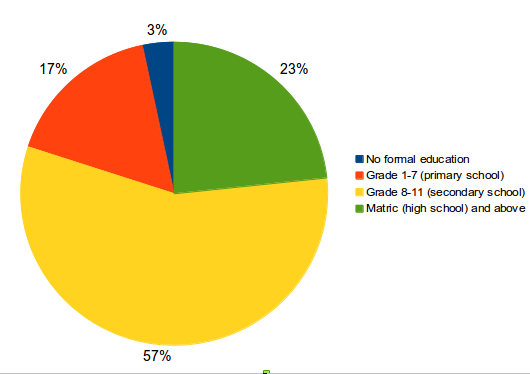
\includegraphics[width=0.6\textwidth]{Figures/education_level.png}
    \rule{35em}{0.5pt}
  \caption{Participants' income distribution.}
  \label{figure:education_level}
\end{figure}

\begin{table}[h!]
  \begin{center}
    \caption{Ethnicity of contextual inquiry's participants}
    \label{table:ethnicity}
	\begin{tabular}{|p{3cm}|p{4cm}|p{2cm}|}
		\hline
		\textbf{Ethnicity}&\textbf{No. of Participants}&\textbf{Percentage}\\
		\hline
		 Black African&8 &26.67\% \\
		\hline
		 Coloured&22& 73.33\%\\
	\hline
	\end{tabular}
  \end{center}
\end{table}

\begin{figure}[htbp]
  \centering
    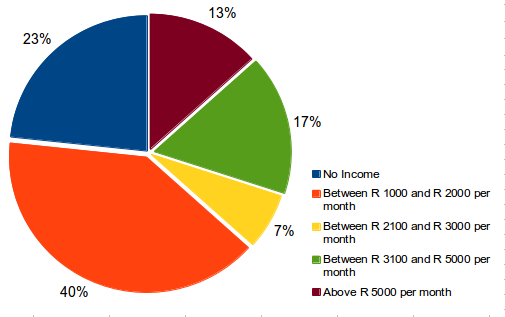
\includegraphics[width=0.6\textwidth]{Figures/income_distr.png}
    \rule{35em}{0.5pt}
  \caption{Participants' income distribution.}
  \label{figure:income_distr}
\end{figure}

Most of the participants were either overweight or obese with an average body mass index (BMI) of 33.36 kg/m\SP{2} (standard deviation of 5.74 kg/m\SP{2}). The average age was 53.13 years old (standard deviation of 11.77 years old).  Almost 86\% (26) were above 40 years of age. This means we were dealing with old participants and hence this group had a tendency of being inexperience or less conversant with technology.

\section{Data Collection Methods and Analysis}
We used a semi structured questionnaire to interview participants. Each participant was interviewed for a period of 20 to 30 minutes. The questionnaire had four groups of questions and these included: demographics; cellphone ownership and utilization; access to information and pedometers; and barriers to diet and physical activity. 

I used both descriptive statistics and qualitative approaches to analyse the information obtained from participants’ responses. Although our objective was to interview overweight and obese patients only but we included few participants who appeared to be thin but were diabetic. Since diabetes is a lifestyle related disease, we found that it would be interesting to also understand utilization of cellphones, and access to information even to individuals who appear not to be overweight but these individuals may had some input on various issues related technology utilization, and  barriers to adoption of healthy behaviours. All the names that are used in presentation of findings are just pseudonyms to protect privacy of participants. 
\section{Findings}
\subsection{Utilization of Cellphones}
Twenty nine out of thirty participants owned cellphones. The most used services were SMS and voice with at least 80\% of the participants using each of the two services. It was found that at least 60\% of the phones owned by participants were smart-phones (Figure \ref{figure:cell_ownership}), but utilization of functionality/services that are supported in smart-phones appeared to be lower relative to voice and SMS (Figure \ref{figure:cell_utilization}). Utilization of smart-phone supported services appeared to decrease with age. Utilization of Whatsapp appeared to be higher compared to other services that are specific to smart-phones. What led to adoption of Whatsapp is that participants were influenced by family members and friends who were already in Whatsapp. These influencers suggested Whatsapp as to be cheaper than SMS. For instance one male participant aged 47 years of age heard that Whatsapp was cheap for communication, and his son helped him on loading it into his phone. Therefore, in this context, social influence played a role in adoption of some smart-phone supported services. There is a positive correlation between social influence and adoption of high-tech innovations \citep{vannoy2010social}.  

\begin{figure}[htbp]
  \centering
    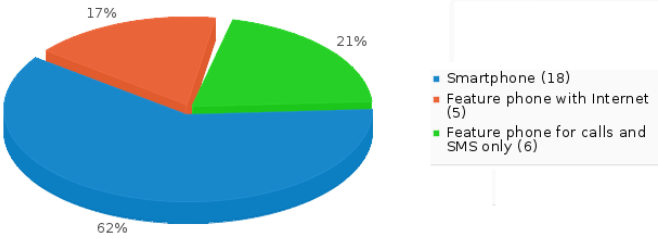
\includegraphics[width=0.5\textwidth]{Figures/cell_ownership.png}
    \rule{35em}{0.5pt}
  \caption{Participants' phones types.}
  \label{figure:cell_ownership}
\end{figure}

\begin{figure}[htbp]
  \centering
    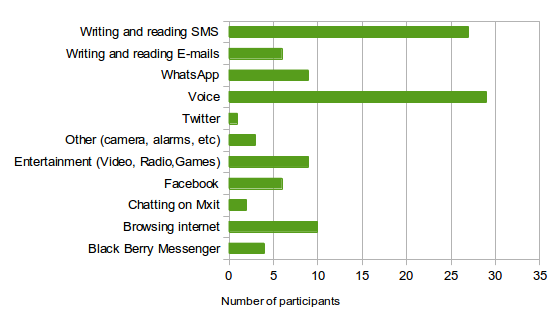
\includegraphics[width=0.5\textwidth]{Figures/cell_utilization.png}
    \rule{35em}{0.5pt}
  \caption{Participants' phones types.}
  \label{figure:cell_utilization}
\end{figure}
\subsection{Help Seeking in Utilization of Cellphones}
There were several scenarios of informal help seeking in utilization of cellphones as highlighted on Table \ref{table:intermediated}. Majority of the participants had solicited  informal help from other people before, in tasks such as: (1) to configure services/apps on their phones (e.g. Whatsapp, Facebook); (2) habituation of skills required for utilization of various functionality (e.g. a phone book of a new or unfamiliar cellphone, Whatsapp); and (3) to interact with certain features such as SMS, Internet browsers, and etc.

There was a variation in the degree of help-seeking and it was determined by how often participants wanted to execute unfamiliar tasks. Tasks such as configuration of services and apps or teaching of individuals had rare occurrences as they only happened when participants had encountered a new application or device and they don't know how to make it functional. 

\begin{table}[h!]
  \begin{center}
    \caption{Scenarios of intermediated interactions}
    \label{table:intermediated}
	\begin{tabular}{|p{1cm}|p{12cm}|}
		\hline
		 \textbf{No.}&\textbf{Scenario}\\
		\hline
		 1& She is being helped to read SMSs by her \emph{daughter}, but she could do it on her own when the daughter is not around. \\
		\hline
		2&He doesn’t know how to reply back to an SMS. So his \emph{grandson} always helps him with that.\\
	\hline
	  3&Her \emph{children} or  \emph{work colleagues} could help her to read SMS written in English that are received through her feature phone. She also mentioned that her two children were skilled in operating cellphone more than her and one of them had a Black Berry smart-phone.\\
	  \hline
	  4&He can take photos using his mobile phone’s camera but he doesn't know how to save those photos on a memory card. His \emph{son} helps him with that once in a while. But, also his son helped him in loading Whatsapp on the phone.\\
	  \hline
	  5&Her \emph{children} have taught her on how to use Whatsapp, take video etc. Now she is learning on how to record sound, set reminders on the phone for insulin and medication.\\
	 \hline
	 6&The \emph{son} would help her to interact with USSD service for checking loyalty points on MTN. MTN is a mobile communication service provider operating in many African countries.\\
	 \hline
	7&She was taught her \emph{son} on how to access a phone-book when composing SMS using her new phone.\\
	\hline
	8&She receives assistance from her \emph{helper} when she wants to send messages to her children.\\
	\hline
	9&She was once helped to do set-up her new phone at a cellphone shop. She was also taught on how to operate BBM by her \emph{grandson}.\\
	\hline
	10& He was once taught on how operate Whatsapp by his \emph{niece}.\\
	\hline
	11&Her \emph{son} and \emph{grandson} have once helped to configure Whatsapp and Facebook on her phone. They have also taught her on how to use those two web services. In addition, she also asks the son to search for certain health information on the Internet, and once the search is done the the son would pass the phone to her to view that information. This happens once in a month.\\
	\hline
	12& Her \emph{son} and \emph{grandson} always teach her on how to use various functionalities like games etc., but she is not so much keen on operating those functionalities. She also admitted that her son and grandson are so much interested with their mobile phones and they spend a lot of time playing using phones something that she doesn't understand.\\
	\hline
	13& This participant didn't own a cellphone. She had no formal education and she was unfamiliar with how to operate a cellphone. Her son receives SMS directed to her and reads it aloud for her or translates an SMS to verbal communication. Also, the son receives phone calls and hands over the phone to her when the person on the other side of the line wants to speak to her.\\
	\hline
	\end{tabular}
  \end{center}
\end{table}
\subsection{Selection of Help Givers}
Participants chose trusted individuals to act as their help givers, typically their children and grandchildren or, less often, children of relatives, family friends, or someone at a cellphone shop. Preference on who is likely to be solicited to assist favours family members. Help givers are selected based on the merit of skills/competence, and interpersonal trust based on a social relationship, and past experience of help seekers on specific help givers.
\subsubsection*{Interpersonal trust}
Interpersonal trust in this context means that whether help-seekers may feel comfortable to seek help from specific people or not. Privacy and existing relationship between a help-seeker and help-giver were first concerns when deciding of who should be asked for help. In additional to that, there was also trust on whether a helper giver may be willing to deliver when solicited for help and this was influenced by experiences in past attempts to seek help. Experiences on past attempt to solicit help refers to help-seekers' positive and negative experiences as an outcome of seeking help. These experiences shaped perceptions of some of the participants towards seeking help with cellphone or any other technology. For instance, one female participant aged 67 years old reported that her daughter helped her once but she had no patience. A male participant aged 47 years of age mentioned that he would like to be assisted on using several services such as MMS, but he thinks that young people may not be having patience to help. Such negative experiences can hinder future help-seeking behaviours from specific help givers. This resonates with the following finding by~\cite{kiesler:twi}, parents may be hesitant to seek informal help from their children after encountering negative experiences.
\subsubsection*{Help-givers' Competence}
In additional to interpersonal trust, the decision of who should be solicited for help was also influenced by help-seekers' level of trust on skills possessed by help-givers. Participants had confidence on competence of their children in using cellphones. Several participants sees their children as having technical know how skills in using cellphones. For instance one 31 years old female participant mentioned that her five years old son knows how to navigate through her whole phone and use it more than what she can do. Another female participant aged 56 years of age explained how children are eager to teach her various things on a cellphone but she is not so keen in engaging to cellphones like they way her son and grandson do. A forty seven years of age male participant also mentioned that young people in their families are more skilled in cellphone than old people.
Participants reported that their kids were borrowing their phones to do other tasks and this demonstrated that their kids had better skills with technology. Scenarios of sharing are presented on Table \ref{table:phone_sharing_contextual} below. 

\begin{table}[h!]
\begin{center}
    \caption{Scenarios of sharing of cellphones between participants and their children}
    \label{table:phone_sharing_contextual}
	\begin{tabular}{|p{1cm}|p{12cm}|}
		\hline
		 \textbf{No.}&\textbf{Scenario}\\
	\hline
	1&``Zandile'', a 47 years old female participant, mentioned that her 16 years old son could borrow her phone to use MXit. But herself she is not using anything else on the phone apart from calls and SMS. She also mentioned that she is not so much interested with technology. For example she has internet at work, but she is not really using it.\\
	\hline
  2& ``Buyisiwe'', a 31 years old female participant narrated an experience about her five years old son who uses her smart-phone to listen to music. But she has to lock it while he is listening, because it happened at one point that the son deleted almost everything on the phone.\\
  \hline 
  3&``Celine', a 48 years old female participant lends her phone to her daughter who uses it for normal Internet browsing and Facebook. Celine owned an advanced feature phone enabled with Internet but she was not using internet on the phone.\\
  \hline
	\end{tabular}
  \end{center}
\end{table}
In other scenarios participants mentioned that their kids borrow their phones to search for information related to school assignments. These examples demonstrate the level of skills that potential help-givers can have. Trust on skills possessed by help-givers has been found to be very important to individuals seeking help in the ICTD and HCI contexts.~\cite{ramirez2013infomediaries} suggested that empathy and technical skills of infomediaries influence the outcomes of the process of infomediation to users at public access venues. Another study that examined motivations for informal support in utilization of computers at home found out that skills of help-givers to be one of the factors that influence help-seekers to solicit help from specific people~\citep{poole:chh}. 
\subsection{Access to Health Information and Self-Monitoring Support}
We had collected information about access to health information and self-monitoring support among the participants. Informational support in which most the participants relied on is that one provided through face to face meetings with doctors or dieticians during hospital visits. Normal hospital visits are scheduled in intervals of every 3 or six months. But they do visit the hospital only two or three times in a year. In addition to face to face information, patients normally receive paper sheets with information that provide guidance on how to eat healthy. These paper sheets are normally received when patients attend clinic for the first time after being diagnosed with diabetes. Most patients we interviewed were type 2 diabetic and overweight. Doctors and nurses encourage them to eat healthy and exercise. 

Majority of the participant lacked informational support beyond hospital settings that could provide guidance in eating healthy and exercising. Very few participants had used cellphone services as means of querying or receiving information related to health. Only six participant had used internet to search for health information, while only one participant had used a cellphone app for health. Also only two participants had used SMS while only one had used voice to look for health information. Table \ref{table:health_information} shows some of the scenarios of where participants had used ICTs in relation to learning about issues concerning their health.
\begin{table}[h!]
\begin{center}
    \caption{Participants’ usage of ICT to fullfil health information needs}
    \label{table:health_information}
	\begin{tabular}{|p{1cm}|p{12cm}|}
		\hline
		 \textbf{No.}&\textbf{Scenario}\\
		 \hline
		 1&``Anitha'', a female participant aged 56 years old, would send SMSs to her son while he is at his workplace. This SMS is usually a request to check for certain  health information on the internet and the son could print for all the material related to that information that was requested. She also follows Dr Oz program on TV about health stuff. If she misses she would go to the Internet and visit the programme's website\\
	  \hline
	  3& ``Jane'', a female participant aged 36 years old, had an app on her phone for giving health tips. She downloaded that app from the Internet.\\
	  \hline
	  4& ``Maria'', a female participant aged 57 years old mentioned that she uses Facebook. She has three diabetic friends and they share diet concerns, recipes, and discuss diabetic specific issues that they experience . They don't discuss about exercise. She sometimes searches on Google about medications especially when she starts using new medications. She uses Google to get more information on the things her doctor advises on.\\
	  \hline
	  5& ``Evelyn'', a female participant aged 63 years old, subscribes to health websites to receive emails with health tips and information. She sometimes calls a dietician to ask about certain diet information.\\
	  \hline
	\end{tabular}
  \end{center}
\end{table}

Self-monitoring of blood glucose seemed to be common among the participants because many of them were diabetic. Self-monitoring of other health parameters such as diet and physical activity seemed not to be done by many participants. Out of thirty participants we interviewed, only two participants had used a pedometer before.  One participant reportedly to use a gym bicycle with a meter that can show distance cycled but she has abandoned using it. Only eight participants reported that they have used a diary before to record the food they have eaten. But this recording is not consistent. Some have stopped doing it although they claim that when they visit hospital, sisters (nurses) always remind them to record foods they have eaten. This food recording is mainly for controlling the levels of blood glucose. For instance, one participant mentioned that she has a note of where she records the blood glucose before she eats and the blood glucose after she has eaten. So she records what she has eaten and the blood glucose levels before and after meals. But overweight and obese diabetic patients are also encouraged to lose weight. Because losing weight has an advantage of lowering levels of blood glucose.  And the only way to lose weight is to follow the recommended diet and become more physically active. 
\subsection{Barriers to Adoption of Healthy Behaviours}
The research teams also examined on barriers to adoption of healthy behaviours i.e. healthy diet and exercises.

On barriers towards adoption of healthy diet, 76\% of the participants mentioned that the recommended healthy food is always expensive. For instance fat free foods are much more expensive compared to full fat foods. One participant associated eating of certain food to cultural upbringing. She explained that Muslims in Cape Town often have very high fat and high sugar content foods  such samosas. One of the comments that appeared to be common to many participants is that; it is difficult to have a budget for separate meals within the family, because diabetic members always have their diet food which seems not be preferred by the rest of the family. So diabetic members might end up eating what the rest of the family eats. They do try to have diet foods by it is not always manageable. But one participant who seemed to be highly motivated disagreed with that argument and said most people lack an understanding of what carbohydrate means. She further mentioned that, education about diet should be contextualized to terms that people are already familiar with. She said most people don't understand what is said by dieticians because it is not communicated in the context they understand. For example the concept of carbohydrates is not well comprehended by many people. But if the topic is well explained using what is already familiar to patients, then they are more likely to comprehend it.

On the question of perceived barriers to physical activity, nine(9) participants mentioned that lack of time to do physical activity because of a busy schedule contributes to less exercising. This is supported by some remarks shared by participants on Table \ref{table:busy_schedules}. Seven participants mentioned that lack of areas to walk around is one of the perceived barriers to physical activity. The most common comment given out to support this argument was that, most of the areas where they live are not safe for somebody to be out walking all the time (Table \ref{table:safety_issues}). Most of these areas have high rates of crime.

\begin{table}[h!]
\begin{center}
    \caption{Excerpts on observation of common participants’ remarks on association between being less active and busy schedules}
    \label{table:busy_schedules}
	\begin{tabular}{|p{2.5cm}|p{10.5cm}|}
		\hline
		 \textbf{Participants}&\textbf{Remarks}\\
	  \hline
	  1&She goes to work very early in the morning and comeback late at night.\\
	  \hline
	  2&Difficult to manage work and household.\\
	  \hline
	  3&She goes to work at 4.00 AM and come back at 7.00 PM. She works for 6 days in a week.\\
	  \hline
	  4&She looks after the family. She takes her sisters child to school, also she does the cooking. She does a lot of house work. So it is difficult to have a planned series of physical activity.\\
	  \hline
	 5&Difficult to balance between planned session for physical activity and manage both work and household at the same time.\\
	 \hline
	 6&Busy with house work at home.\\
	 \hline
	\end{tabular}
  \end{center}
\end{table}

\begin{table}[h!]
\begin{center}
    \caption{Excerpts on observation of participants’ remarks on safety concerns on areas to do walking or running}
    \label{table:safety_issues}
	\begin{tabular}{|p{2.5cm}|p{10.5cm}|}
		\hline
		 \textbf{Participants}&\textbf{Remarks}\\
	  \hline
	  1&The neighbourhood is not safe to wonder around.\\
	  \hline
	  2&It is not safe in her area. She doesn't like to be outside most of the time.\\
	  \hline
	  3&It is unsafe at night and early morning.\\
	  \hline
	  4&The area where she stays is not safe to walk around.\\
	  \hline
	 5&Not safe to walk alone. She prefers to walk through houses.\\
	 \hline
	\end{tabular}
  \end{center}
\end{table}

But despite the claim of lack of both time and areas to exercise these participants mentioned that they been active when doing their daily errands (Table \ref{table:daily_activity}). 

\begin{table}[h!]
\begin{center}
    \caption{Excerpts on observation of participants' remarks regarding physical activities that were part of their daily lives' routines}
    \label{table:daily_activity}
	\begin{tabular}{|p{2.5cm}|p{10.5cm}|}
		\hline
		 \textbf{Participants}&\textbf{Remarks}\\
	  \hline
	  1& She walks from home to visit relatives and friends.\\
	  \hline
	  2&He only walks when he goes to church.\\
	  \hline
	  3&She walks to from her home to a bus station everyday and walks a lot at her work place, so it would be great for her to have something to keep track of how much exercise she gets. She wants to be more active but works 7 days a week.\\
	  \hline
	  4&She exercises in a group of people for three times a week and she now feels much healthier. They have a "biggest loser" competition going at the moment. She would like to have a pedometer to keep a better track of her activity.\\
	  \hline
	 5&She walks only when she has to. She only walks up and down in kitchen. She has a treadmill, but she doesn't use it.\\
	 \hline
	\end{tabular}
  \end{center}
\end{table}

\section{Contextual Design Insights}
These are some of the design insights that were uncovered from the aforementioned findings. In this context, majority of the participants were not utilizing ICTs in self-management of their health as they relied only on paper diaries. The only parameter that was being monitored by majority of the participants was blood glucose since all participants were diabetic. Blood glucose is usually controlled through many factors such as diet, exercise, and medication. Type 2 diabetes is linked to obesity and its self-management is mostly through diet and exercise.  The process of self-management can be very cumbersome if it is done using pen and paper and this may reduce compliance \citep{mattila2008mobile}. A paper diary may not be as effective as an electronic diary when it comes into navigating across behaviour patterns for the purpose of self-reflection. Therefore, personal health apps may be important in supporting self-management of health. However, these personal health apps may not be very useful in this context considering the fact that majority of the participants have limited skills in operating technology. The findings above indicate that some participants with limited skills seek help from people with skills. But this approach has its limitations as it relies on existing intrinsic motivation of help givers. Long term usage is crucial for compliance~\citep{mattila2008mobile}, but one cannot achieve this long term usage in the context where a technology needs to be utilized through help givers while most technologies were not designed to anticipate utilization through help givers as part of the usage ecosystem. As it has been advocated that novel approaches such as ICTs in lifestyle modifications may facilitate moving of management of lifestyle-related chronic conditions from healthcare system to citizen-centric health promotion and disease prevention interventions~\citep{korhonen2010personal}; hence it is important for one to think of how we can design technologies that can scale to demographics that are not well-considered in traditional interface design. 

There are several decisions that were crucial to the design of the first prototype.  Since participants reported to have activities related to NEAT (non-exercise activity thermogenesis) in their daily life, then  the first decision was based on the idea to promote NEAT since they have proved to be beneficial in improving well-being. The second consideration was about  promoting of health eating habits using a metaphor that was already used by dietitians. In order to educate patients, dietitians used a meal chart to reflect how a plate with a health meal looks like. The third design decision was on how to design motivational affordance to support collaboration between help seekers and help-givers. This was inspired by the finding about sharing of phones between adults and kids. The finding indicated that kids borrow phones from their parents because they are motivated with specific things on the phone. Some of those things were social media, games, music, etc.. Therefore, if one could design a system that afford specific motivational affordances that address needs of kids and integrate those affordances with self-monitoring of behaviours of adults, then it is possible to enhance motivation of kids to help their parents with self-monitoring tasks. With the guidance of self-determination theory, and techniques that have been used in the previous studies that utilized gamification (described on the \emph{Literature Review} chapter), a prototype was developed. The iterations of prototype development and subsequent evaluations are discussed in the next chapters.

\begin{flushright}
\end{flushright}
% Chapter 1

\chapter{Prototype I} % Main chapter title

\label{prototype1chapter} % For referencing the chapter elsewhere, use \ref{Chapter1} 

\lhead{Chapter \emph{Prototype I}} % This is for the header on each page - perhaps a shortened title
%----------------------------------------------------------------------------------------
\section{Development of the Prototype}
The initial task was to develop the first version of the application prototype. The prototype had features that allow monitoring of physical activity and diet of an individual. The manipulation of user interfaces of the app was specifically targeted to help givers/intermediary users. The prototype was designed to encourage one help-giver to work together with one help-seeker by forming one pair of users. In order to make the act of helping to be perceived as both important and meaningful by intermediary users, the first message displayed when opening the app was explicit that an intermediary user is helping someone they know to manage their wellness. In the case of motivating ongoing use, the app had included gamification features of where each pair could be awarded points, badges, nice looking gardens, and fish tanks. The essence of having these features was to enable pairs of users to have a set of challenges that will promote competence which is one of the core aspects of self-determination theory. In addition to the aforementioned features, within each pair of users' garden and fish tank, there was a Facebook social plug-in that could allow members from different teams/pairs to comment on or like each other. The presence of these social features was to promote relatedness which is also one of the aspects of self-determination theory. Facebook groups were also utilized to give feedback or remind users to engage with the application. The first prototype didn't explicitly have any functionality to support autonomy. Ideally, the information flow on the high-level representation of the system to encourage intermediated use was designed as depicted on Figure \ref{figure:prototype_1}. A web app was developed using a combination of several web technologies such as HTML, JQuery, JavaScript, and CSS on the client side while the server side was implemented using Django Python framework. Sample screen-shots of the prototype are shown on Figure \ref{figure:prototype_1_screens}. Authentication was done through Facebook accounts of intermediary users. The pedometer app was developed in Android environment by using open source code which was extended to allow readings from phone's acceloremeter (built in sensor to detect physical activity) that are above a certain threshold to be detected as bodily buonces from physical activity. The data was then stored into SQLITE database on the phone. The code also included libraries for transfering data to the server after every 30 minutes. But users could also press an upload button on the pedometer app for immediate transfer of footsteps to the server. The pedometer was not calibrated to differentiate varying intensity of physical activity as it was not an important aspect for this study. So a single body bounce was treated as one step regardless of its intensity.

\begin{figure}[htbp]
  \centering
    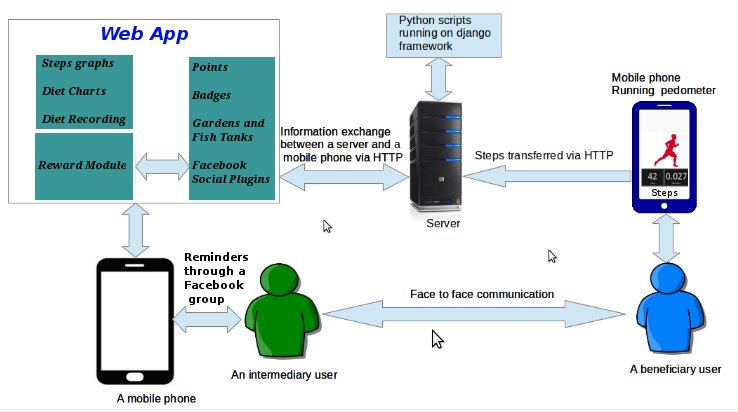
\includegraphics[width=0.8\textwidth]{Figures/prototype_1.png}
    \rule{35em}{0.5pt}
  \caption{Information flow in the first prototype.}
  \label{figure:prototype_1}
\end{figure}

\begin{figure}[htbp]
  \centering
    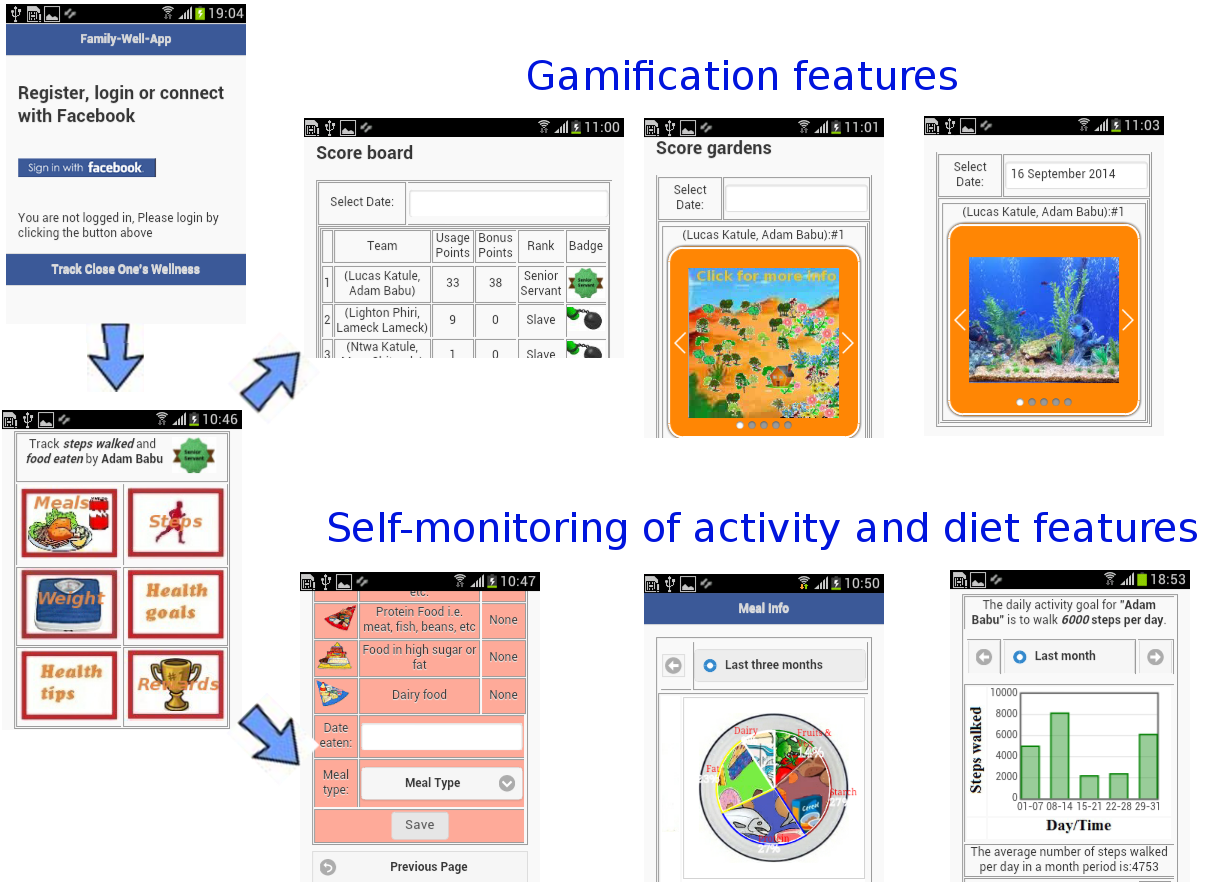
\includegraphics[width=0.8\textwidth]{Figures/Version1/Prototype1Screenshots.png}
    \rule{35em}{0.5pt}
  \caption{Sample screen-shots of the first prototype}
  \label{figure:prototype_1_screens}
\end{figure}

This prototype aimed at encouraging increase in physical activity and  decrease of sedentary behaviours through informing individuals (help-seekers) of their current behaviour trends. In addition, also individuals could monitor whether they were eating healthy or not. Some visualization techniques that are similar to this have been previously used  in systems that were designed for direct users such as ``Fish'n'Steps''\citep{lin2006:fish}, ``Ubifit''\citep{klasnja2009:using},  and ``Few Touch Application''\citep{arsand:mobile}. The idea of using a plate to show distribution of meals' nutrition mimicked a practice that was used by dietitians at the hospital were we conducted the contextual inquiry reported in the previous chapter. In this design metaphor, the amount of each food group that needs to be consumed is presented as a bisector of a pie chart. 
\section{Prototype Evaluation}
There was a slightly change of plan  due to contention about the study design and implications to ethics when dealing with patients as per requirements of Faculty of Health Sciences Human Research Ethics Committee (FHS-HREC) of University of Cape Town. FHS-HREC was interested to have clinical outcomes as one of the expected outputs. These requirements were going to increase the scope of the work of which its main area of contribution was supposed to be in human-computer interaction. Also, the envisaged technology was only under research; hence it was not expected to be comprehensive enough and ready for any clinical trials even after completions of all evaluations that were meant to be carried out throughout this research. Therefore, I had to look for a different group of participants outside hospital settings. This involved reapplication of ethical approval to an institution body different from the first one that approved the study reported in the previous chapter. This time the ethical approval was granted by Faculty of Science Research Ethics Committee (FSREC) of University of Cape Town (see Appendix \ref{AppendixB}).

In order to evaluate the aforementioned prototype, I recruited participants through help from an NGO
based in Cape Town called ``\textbf{\textit{Mamelani Projects}}''\footnote{http://www.mamelani.org.za/}. This NGO was carrying out outreach programs on health education in less privileged
communities. Mamelani was training women on issues of HIV/AIDS, nutrition, and gender equality. 

The NGO helped to recruit participants among people who were part of their trainings in Philippi township. Criteria for recruitment were as follows: (1) participants that were mid-aged and above (contextual enquiry suggested that most prospective beneficiaries could be above mid-aged) and (2) participants must had an intermediary person willing to work with them (someone they trusted or close to them). The NGO identified the targeted participants that met the inclusion criteria. A total of six adult participants were recruited of which both were women above mid-aged (\textgreater= 35 years of age). Each one of the adults brought one intermediary to form a pair. Three intermediaries were girls in between 19-23 years of age. The remaining three intermediaries were boys aged between 14 and 19 years of age. 

Participants were informed of their rights. Participants were also informed of which of their information will be collected by the study. Both adults and their respective intermediaries signed consent forms except for intermediaries who were minors, these signed assent forms that were approved by their respective parents/guardians. 

The next step entailed training of intermediaries on how to use the app. The application was deployed to the field from the end of October 2014 to beginning of December 2014. In order to limit potential complications from deploying the intervention on multiple platforms, each pair of participants was given one Android phone (Samsung GT-S5300) running the pedometer app. Participants were required to utilize the web application hosted at University of Cape Town by using a web browser built into their phones. In order to retain participants in the study each intermediary participant and each beneficiary participant who remained as part of the study received ZAR30 (\~US\$3) worth of airtime every week for the duration of the study. I collected qualitative feedback in the middle and at the end of the study. All the names used in qualitative feedback are just pseudonyms to protect identity of participants.
\section{Findings}
Observations and qualitative feedbacks from the six cases/pairs are presented below. The first three pairs consisted of parents working their children while the remaining three pairs it was just an adult working with either a close or distant relative in each pair.
\subsection*{\textbf{Pair 1: Mother and Son}}
This pair consisted of a boy aged 17 years of age working with his mother. The boy is referred here with the name ``\textbf{Jabulani}'' and his mother is referred with the name ``\textbf{Nandipha}''. Jabulani lived with his mother and other siblings. He appeared to be passionate in engaging with a cellphone. He described the intimate relationship he had with his cellphone.

\userquote{\textbf{Jabulani}} {``There is a time I lost my cellphone. It was like the end of the world to me because I didn't have anything to play with''}

The excerpt above shows that a cellphone could be a source of intrinsic motivation for young users in this context. 

He mentioned that he felt happy helping his mother. He also articulated the reason for helping his mother as that he felt it was his duty since the mother took care of him when he was growing up. 

\userquote{\textbf{Jabulani}} {``I feel happy when I am helping her because she helping me when I was growing up so it is my turn to help her''}

\textbf{Nandipha} also felt very happy being helped by her son and she mentioned that she thinks her son is very brilliant more than her in technology and she gets to know things because of him. 

Jabulani and Nandipha were the first one to engage with the app for at least three different days. All of a sudden their use stopped. When I asked Jabulani together with his mother of challenges that might have prevented them from using the app, their responses indicated that were more conscious about airtime as it was one of the reasons of why they didn't login more often. So there were times where they ran out of airtime. They thought having more data bundles might solve the problem. Another reason for why they didn't use the app more often is associated with lack of competitions from other pairs and also they had accomplished the highest challenge within few days. In the first few days they were so curious about attaining the highest badge. Jabulani claimed that her mother was walking up and down so that they reach that goal. Jabulani discussed with his mother that they must reach that goal in  a week. They managed to reach the goal and there was no more boundary to break.

Badges were one source of motivation to this pair. Jabulani felt motivated by the badges and he was persuading his mother to work harder so that they reach the highest badge which was Queen/King.

\userquote{\textbf{Jabulani}} {``We talked me and my mum that we must not reach only for today but for the whole week. That was our goal to reach the queen and the king for the whole week. I remember a day that was the best day. My mum woke up very early to walk around, to go to Philippi Makasikava [A location within the neighbourhood] just to reach that goal''}

Also Jabulani noticed something on the scoreboard. He and his mother were there leading. Another team (Pair 3) was in the second position. The third position was held by Pair 4. Then after few days Jabulani noticed that Pair 4 moved from a third position to a second position. So Jabulani told his mother that ``we must not drop down because they (Pair 4) are going to reach us''. In that context competition with others was a source of motivation for Jabulani. Although Jabulani was helping his mother but he thought like the ownership of the winning process as theirs because he used the word “We” all the time to imply that he felt that he was part of that process. Additionally, Jabulani enjoyed information displayed by a botanical garden and a fish bowl. He explained why he was so interested in such abstract visualizations. When he was growing up he used to watch cartoons. So when he sees those pictures of trees and fish he feels he is part of that process of making those images/cartoons. So drawing fish and trees through their team's performance motivates him more and he tells his mother that they must have more fish in the bowl. Also the idea of fish in the bowl motivated Nandipha to walk more. She mentioned  that she didn't like to see her bowl empty without any fish, so she tried to walk more steps as she could. These ideas of abstract visualization such as fish bowls/tanks and garden have been previously used in systems that involved only one user on interaction with user interfaces in aforementioned systems such as Fish'n'Steps\citep{lin2006:fish}, Ubifit Garden\citep{klasnja2009:using}, etc., the only difference in this context is that, the same ideas were extended and tested with two users who were collaborating to attain one objective.
\subsection*{\textbf{Pair 2: Mother and Son}}
``\textbf{Dumisani}'' was a 14 years of age who lived with his mother, ``\textbf{Kholiwe}''. Dumisani was acting as an intermediary for Kholiwe. Dumisani and Kholiwe used the system for only the first three days and they dropped out. On responding to the question of why was it the case, Kholiwe mentioned that it was the inability to access the system every time they tried out. The web page was always giving them time-outs and this discourages them from trying. But it was also observed that Dumisani was not very familiar with Facebook authentication as he didn't have an account before. I created one account for him of which it wasn't very helpful. The decision in using Facebook authentication was based on an assumption that all intermediaries may have Facebook accounts which was not the case. However, despite technical challenges this pair also showed enthusiasm in using the app.
\subsection*{\textbf{Pair 3: Mother and Daughter}}
``\textbf{Zama}'' who was a 20 years of age was supposed to act as an intermediary for her mother, ``\textbf{Fikile}''. Since the daughter appeared to be interested to help her mother, then one would think that intermediation is possible. Unfortunately, the two lived in different houses and they never used the system at all. Their contact to discuss issues about the system was limited as Zama was raising a toddler at that time. In addition, Fikile appeared to had some expertise in using technology as she already was using Facebook, therefore she was interested to learn how to operate the system on her own but she failed because of the situation of her daughter. However, the system had been set up only to allow Facebook account for Zama. 
\subsection*{\textbf{Pair 4: Close Relatives}}
``\textbf{Lindiwe}'' was a young girl in her early twenties. Lindiwe was acting as an intermediary for her auntie ``\textbf{Nceba}'' but they never lived together in the same house. The pair had not been interacting with the application at all. When I interviewed Nceba of why they were not using the app, her response was that she doesn't know how to operate it on her own and her intermediary seems not  to be around most of the time. She is curious to access the information but her intermediary seemed not to be cooperative. So she suggested to bring someone else who was also a close relative.
\subsection*{\textbf{Pair 5: Close Relatives}}
``\textbf{Neliswa}'' was a girl aged 23 years of age. Neliswa  was acting as an intermediary for her auntie ``\textbf{Nkosazana}'' but they lived together in the same house. The pair had not been interacting with the application at all. I never had a chance to interact with this pair since they were not available. But from a personal observation during recruitment, Neliswa appeared to be less interested in the intervention even though she signed the consent form to participate. 
\subsection*{\textbf{Pair 6: Distant Relatives}}
``\textbf{Nkululeko}'' was a boy aged 19 years of age. He was acting as an intermediary for her distant relative, ``\textbf{Noluthando}. Nkululeko and Noluthando didn't live so close to each other but they did see each other more often. System logs showed that this particular pair had not been engaging with the application. I interviewed both of them to find why that was the case. Nkululeko pointed out number of things. The first one was that he tried to access the application a couple of times but he was unable to proceed after login. He was using his personal phone. I checked his personal phone and I discovered that his web browser was the problem. He had never tried to do it using the experimental phone that was in possession of Noluthando. We tried together and it was okay on the other phone.  But in addition to phone's problems he claimed to be busy with school. Despite him being busy, and his phone not being able to support the application,  the absence of things like reciprocal benefits  and a close social relationship with the beneficiary, might be the cause for his low intrinsic motivation in engaging. The previous user, Jabulani had a problem of accessing the application using his personal phone but he made an effort to access using the phone  given to his mother. So the closeness/bond of the two sets users might be the base for the network effect to happen.
\section{Discussion}
Only two pairs of users engaged with the system for more than two days. Both of these two pairs consisted of a beneficiary and an  intermediary living in the same house. These pairs consisted of mothers working with their sons. One of these two pairs was very motivated and enthusiastic about the system. But after some time they also got bored because they were not getting any competition from other teams and they had attained all the challenges within a short period of time. In a third pair, a girl was working with her mother but they were not living together so it was difficult for her to commit to the application. Intermediaries from the remaining two pairs showed little enthusiasm in the project. There were three hypotheses for this lack of enthusiasm to engage with the system and these were: (1) due to lack of motivation to engage with the system; (2) lack of a prior social relationship between the two users within each pair; and (3) Low frequency of interactions between the two users within a pair due to distance.

There was an indication that a prior social relationship is instrumental for intermediaries to perceive value in the act of helping their beneficiary users. In this case the interaction became more meaningful. It also becomes easier for the two users within a pair to negotiate for interaction. For three pairs that consisted of mother/son or mother/daughter there was a tendency for the two users to show the eagerness of working together. For three pairs where members of a pair didn't  have a parent/child relationship, intermediaries showed little enthusiasm in the intervention. Another advantage of a prior social relationship comes to sharing of phones. It was observed that it was easier for an experimental phone to move from a beneficiary to an intermediary when a parent and child were involved in a pair. There was a form of trust that existed between the two users with a prior social relationship. In addition, intermediaries had more authority when they were helping a person who was close to them. If a pair with a prior social relationship needed to interact with the app, then the frequency of these interactions depended on proximity between the two users. For cases where they cohabited or lived nearby it increased the chances of face to face meetings and negotiation for interaction. For instance, ``\textbf{Zama}'', an intermediary participant aged 20 years old was working with her mother. The challenge with this pair is that they didn't cohabit and Zama had a toddler hence this lowered her ability to participate in the intervention.  

Prior social relationship also worked in parallel with the presence of interest to use the app/gamified features. A combination two factors played a some role in  encouraging the two users within a pair to collaborate when they met. For instance , in the case of of Jabulani and Nandipha (mother and son), they discussed about strategies to win against other pairs. Although Jabulani was helping his mother but he thought like the ownership of the winning process is theirs because he used the word ``We'' all the time to imply that he felt that he was part of that process. In addition, if intermediaries are motivated they can become persuaders of beneficiaries that they have a prior social relationship with as it can be seen on Jabulani who encouraged his mother to walk more steps.

There were some drawbacks in utilization of this prototype. From participants' perspective , intermittent internet connectivity, insufficient airtime, less motivated intermediaries, and lack of competition/challenges with others in the gamified system were the key issues mentioned. Other factors include how often the two user meet (Whether they cohabit or they meet more often), and reminders were not timely. I had very high expectations that Facebook reminders will work for this community. An assumption was that every intermediary is probably using Facebook. Actually this was not the case. There were some intermediaries who had never engaged with Facebook before. And the ones who had engaged with Facebook were not doing it so often as I anticipated. For instance ``Jabulani'' had never used Facebook before. ``Jabulani'' was only engaging with Facebook at most twice in a week. Therefore, Facebook might not be an on time-platform for delivery of reminders or any messages to intermediaries in this context. Findings from this informative evaluation led to another iteration in the design. It also informed the manner in which evaluations in chapters \ref{prototype2chapter} (Prototype II) and \ref{summativeevalchapter} (Summative Evaluation) were conducted.
%\begin{flushright}
%\end{flushright}

% Chapter 1

\chapter{Prototype II} % Main chapter title

\label{prototytpe2chapter} % For referencing the chapter elsewhere, use \ref{Chapter1} 

\lhead{Chapter \emph{Prototype II}} % This is for the header on each page - perhaps a shortened title

%----------------------------------------------------------------------------------------
\section{Prototype Development Iteration II}
I started the next iteration of prototype development that aimed to improve the first prototype described in the chapter \ref{prototype1chapter}. In the second prototype the emphasis was more on improving support for the three psychological needs from self-determination theory \citep{ryan2000:self} which are relatedness, competence, and autonomy. I substituted Facebook social plugins with features that could allow users to directly comment on or like each other. Facebook social plugins failed to integrate seamlessly with the app since the network signal was a bit poor in the area where I conducted experiments, therefore users failed to load them into the app. In addition, the system comprised SMS reminders and feedbacks instead of Facebook based reminders. The new system (Figure \ref{figure:prototype_2_screens} ) had the following features of which most of them were improvements from the previous prototype:
\begin{enumerate}
\item{Recording of meals} consumed by a beneficiary user.
\item{A pedometer} for detection of steps walked by beneficiary user.
\item{Pie charts} that show summaries of food groups consumed by a beneficiary user.
\item{Bar charts} that show steps walked by a beneficiary user (daily intervals, 7 days intervals, and, weeks of a month intervals).
\item{Avatars} that can be changed in order to increase autonomy of intermediary users.
\item{Badges} that can be earned through a combination of steps walked by a beneficiary participant and the number of days they app has been utilized by a pair of users. In the previous prototype it was easier to jump from the lowest badge to the highest without passing through intermediate badges as longer as a pair had enough clicks. Therefore, to move to a higher badge in this second prototype a pair was required to use an app for a certain number of days and then couldn't by [ass any badge as the process was incremental. To reach the highest badges pairs were required to pass through all the badges in between in different days, and also to meet requirements for the King/Queen badge which were at least an average of ten thousand (10000) steps walked by a beneficiary user in a day, and at least 18 days of usage activity detected from the app. 
\item{Score board/ leader board} of which points were earned by averaging between points scored from usage (i.e each day of usage resulted into 1000 points earned) and points earned as the result of beneficiary's average number of steps walked (i.e. if the average is \emph{n} steps/day then the number of points accumulated is ``n'')
\item{Botanical gardens} that consisted of trees and flowers. Trees on the garden grows proportional with badges while flowers grows proportionally with number of meals recorded. if a recorded meal contains fruits and vegetables it is an added advantage.
\item{Fish tanks or bowls / Aquarium} that consisted of Fish of different species. Number of species grows proportional with badges while the size of each specie is proportional to number of meals recorded. If a recorded meal contains fruits and vegetables it is an added advantage on the size.
\end{enumerate}
\begin{figure}[htbp]
  \centering
    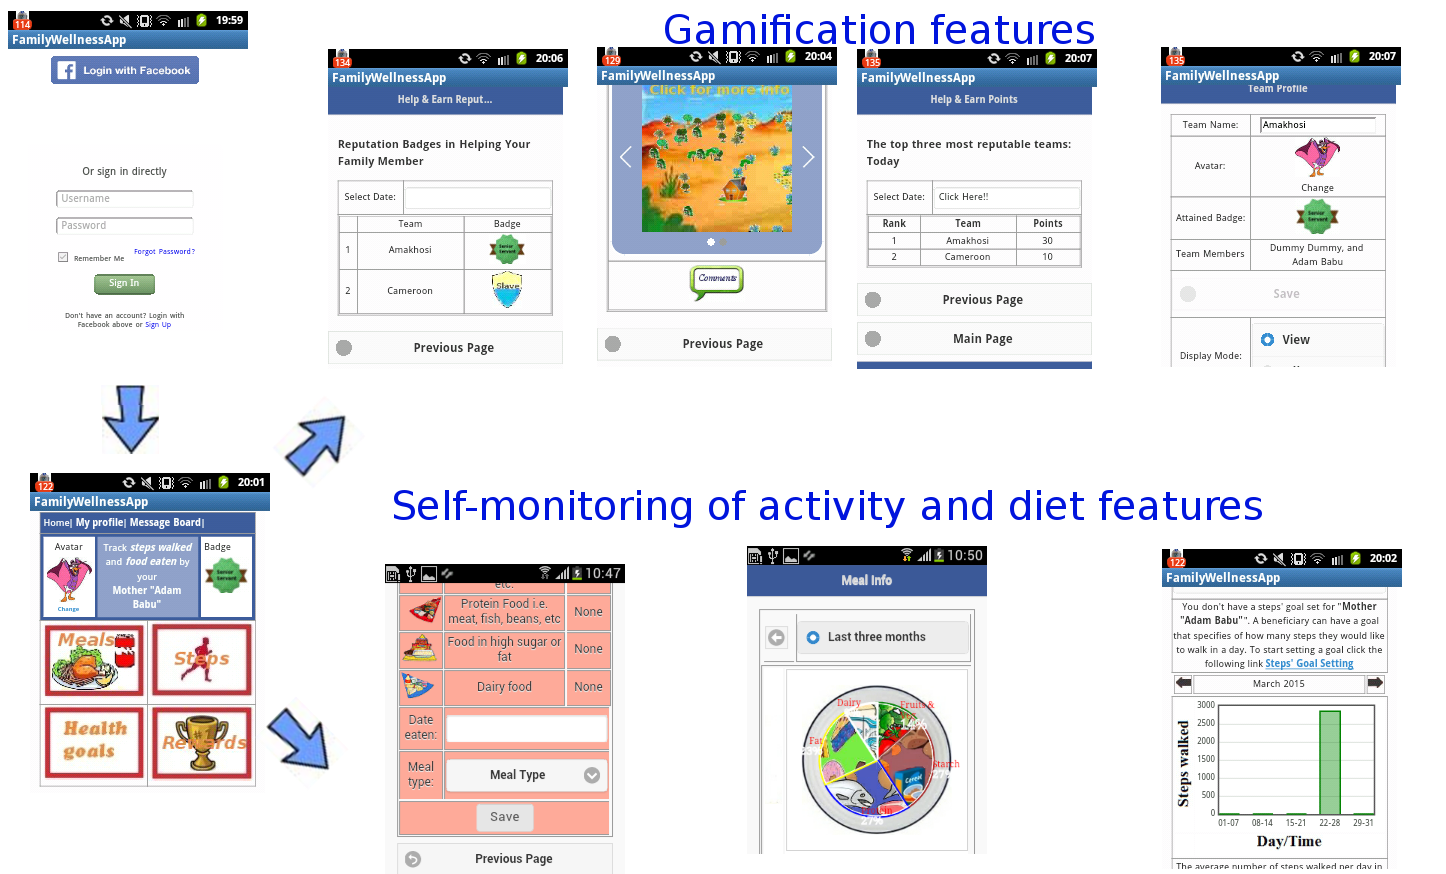
\includegraphics[width=0.8\textwidth]{Figures/Version2/Prototype2Screenshots.png}
    \rule{35em}{0.5pt}
  \caption{Sample screen-shots of the second prototype}
  \label{figure:prototype_2_screens}
\end{figure}

These rules were just arbitrary. The objective was to design challenges with an objective of increasing engagement between intermediaries and beneficiaries when the two users negotiate for interaction with the app.
\section{Prototype Evaluation Description}
The plan in evaluation was to recruit another group of participants. The NGO facilitated access to a group which resided in another side of Philippi where evaluation of the first prototype was conducted. The recruitment was facilitated by the same NGO in Evaluation. But the plan didn't materialize as the NGO advised that we try to look for a different group because the group they were working with expressed concerns regarding safety issues after they heard that they were going to be given phones to use throughout the evaluation period. The NGO was concerned of safety of researchers since rumour had spread throughout the community that someone is going to bring phones to that area. This poses risks to both prospective participants and the researcher. In response to that, this plan was revised and the researcher found another township called Langa, which was a bit smaller and more central township, safer than Philippi.

A research facilitator who is a resident of Langa helped with the recruitment process. This time the recruitment criteria were more stringent compared to the previous evaluation. One of the criteria was to have intermediaries that cohabit or live nearby the beneficiaries. Preference was given to school going children as there were more likely to be interested in gamification. A total of nine adult participants were recruited for the study. The distribution between male and female was three(3) and six(6) respectively. Their average age was 49.3 years old (SD=7.9 years). Each adult participants brought one intermediary participant and formed a pair. The distribution of intermediary participants by gender was 3 males and 6 females. The mean age of these intermediary participants was 14 years old (SD=4.3).  Eight adults  were relatives/familial related to intermediary participants while the remaining adult was just a tenant of her intermediaries' grandmother. Eight intermediary participants were school-going children.
log out
Prior to commencement of the study, both beneficiary and intermediary participants were given information about the study. Participants were informed that the study's cellphone will be collecting their information related to usage of the app, step walked,  and diet and this information will transferred to the researcher's computer at University of Cape Town. All participants who were not minors signed informed consent forms while minors signed assents forms that were also signed by their respective guardians/parents.

Once consent and assent forms were signed, one day was allocated to train intermediary participants on use to use the app. After the training each pair was provided with an one android phone ((Samsung
GT-S5300) that contained two native app. The first app was a pedometer which was not displaying any useful information apart from raw steps' data. The pedometer task was to send these steps to a server so that they can be presented  and viewed in a better format through a web application. The second app provided a link to the web application so that users don't have to type a URL every time they needed to access the web app.

In order to encourage participation, each beneficiary participant received ZAR 40 worth of airtime four times in a period of three weeks (ZAR 160 in total). To encourage participation of intermediary participants, each pair was credited 300MB of data to use on the Android phone as it was expected that intermediaries would borrow phones to access other things on the internet that are beyond prescribed uses.

I left the app in the field for three weeks before conducting an evaluation. After three weeks I conducted the evaluation which is described on the next sub-section.
\section{Prototype Evaluation Methods}
The evaluation relied in two approaches which are collecting user logs and interviews. In interviews, all respondents were familiar/comfortable with English, therefore, interviews were conducted in English. A total of three(3) intermediary participants, and five(5) intermediary participants were interviewed. These are the only participants that I could reach to during the time of interviews. These were short interviews which lasted up to 15 minutes for one person. 
\section{Findings}
The key findings were based on social factors and motivational strategies that influenced usage of the app. Some of the findings from this chapter together with findings from the previous chapter (Chapter \ref{prototype1chapter}) have also appeared in a conference paper that I co-authored \citep{katule2016leveraging}.
\subsection{The Role of a Familial Relationship in the Intervention}
As it was observed in the previous chapter (Chapter \ref{prototype1chapter}), a parent/child relationship may be important in implementation of such an intervention. In this case, a prior social relationship was also very important. Intermediaries that were working with their parents were eager to support their parents because they cared about them. 

Usage of each pair  was clustered its respective relationship type as shown on Figure \ref{figure:relation}. There were three three types of relationships:parent-intermediary, relative-intermediary, and not related , with 4, 3, and 1 number of pairs respectively. Usage on each relationship type was measured through three dimensions: (1)~the average number of days per pair; (2)~the average number of sessions per pair; and (3)~the average number of clicks per pair. More usage was observed on pairs with relationship of type parent-intermediary. 
\begin{figure}[htbp]
  \centering
    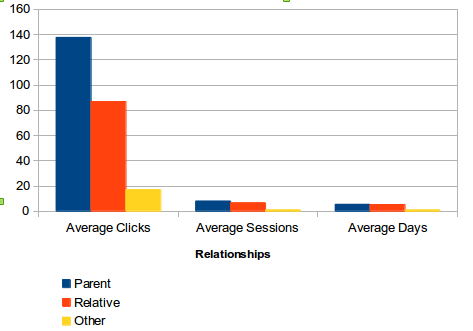
\includegraphics[width=0.6\textwidth]{Figures/relationships.png}
    \rule{35em}{0.5pt}
  \caption{Usage in three groups of relationships\citep{katule2016leveraging}}
  \label{figure:relation}
\end{figure}
In the case of parent-intermediary, or relative-intermediary relationships, negotiation for interaction that initiated by beneficiary users was more possible because of the nature of the prior relationship. For instance the following two scenarios, requests from beneficiaries where always successful most of the time. For instance, \textbf{Zandiwe}, \emph{a beneficiary user, a woman aged 50 years old}, she was working with her sister daughter. Another case was shared by  \textbf{Lulama}, \emph{an intermediary user, a girl aged 20 years old} who was working with her mother, \textbf{Nokanyo}, \emph{aged 57 years old}. 

\userquote{\textbf{Zandiwe}, a beneficiary} {``I used to call Lindiwe like `Lindiwe there is something that I don't understand'. Or I call her the day before when I walk for a long, I call her to come and help me some way somehow.''}

\userquote{\textbf{Lulama}, an intermediary} {``My mother was the one who was pushing me, let’s do it, let’s do it. And we spent more time together. But we are always together around that time I do the app at around o'clock at night. So we talk more than before because she would ask `How am I doing on this?'''}

There were scenarios of whereby a beneficiary user could request assistance at the time where an intermediary wes either resting or occupied by other activities or felt that there was no urgency in fulfilling  such a request. In such a scenario, a social relationship still had to play a role in motivating intermediaries to immediately attend to those requests.

Also for a parent-child relationship,  intermediaries demonstrated sense of being co-owners of the information from the system. For instance, Lulama, used the terms ``we'' or ``our'' repeatedly to describe actions that needed to be carried out by her beneficiary user as actions that needed to be carried out by both of them.
  
\userquote{\textbf{Lulama}, an intermediary} {``When I saw the garden I was like yeah, our garden is looking beautiful. Lets do more. Lets take more steps. Lets eat more veges, because it is the veges and fruits that are important.''}

In addition, intermediaries from pairs with a prior social relationship had more authority in persuading their beneficiaries to do something in order to win. And it was not solely for winning purposes as they cared for health of the people they were helping. This phenomenon was observed in two pairs with the following excerpts.

\userquote{\textbf{Lulama}, an intermediary} {``I am helping her so it [The app] has to mean a lot to me. I am helping her (Nokhanyo) because she doesn't know anything. She is like `What is this?'. This is how you do this. She is like `ooh okay' So it [The app] means a lot to me because I am helping someone I care about.''}

\userquote{\textbf{Nokhanyo}, a beneficiary user} {``Sometimes she used to shout at me. `No no you didn't eat that thing. Tell me what you ate in the morning. I saw you eating this. It seems there is nothing for fruits, peanuts. You must remind me to check you!'''}

\userquote{\textbf{Lwazi} (an intermediary, a boy aged 14 years old)}
{``It [The app] was really good because my 
mother was limiting herself on stuff like pies and fat food. I would tell 
her don't eat this don't eat that. She wasn't eating much vegetables but I 
was encouraging her to eat vegetables''}

It was observed that for pairs that didn't have a parent-child relationship, interactions between intermediaries and beneficiaries where lesser or absent except for cases where an intermediary was motivated by access to the intervention's phone or motivation affordances provided by gamification. But in cases where intermediaries where driven by those factors, still there was some form of a prior social relationship that played a role, i.e. relative-intermediary, although it was not as strong as a parent-intermediary relationship. In these cases, of relative-intermediary relationship, even if the intermediary is not motivated by gamification and the phone, they would still provide infrequent help to their beneficiaries.  In one case where there was no relationship between an intermediary and beneficiary, even the infrequent help was not available i.e. in the case \textbf{Anele} (a beneficiary user, a 47 year old woman, who was working with the granddaughter of her landlord, hence, they were not related. Anele mentioned that every time she passed her request to be helped, her intermediary claimed to be busy and kept on procrastinating by saying they will do it the next day and when that day comes it was the same thing. 

Therefore, a familial relationship played an important role in mediating motivation of some intermediaries to help. 
\subsection{Sources of Motivation for the two Sets of Users}
In cases were both users of a pair were motivated to use the app and there was a prior social relationship between them, then a pair tended to interact in a more playful manner which brought the two users closer compared to before using the app. This happened in  when an intermediary was reporting back the information to a beneficiary user.  This made the interaction between an intermediary and beneficiary to be more enjoyable and less tense. These narration from participants describe how the interaction  between an intermediary and beneficiary was enjoyable, when the two users were engaging with the app.

\userquote{\textbf{Zandiwe}, a beneficiary} {` When she got time, when she is done with her homework she comes and sees the app. And then laughs at me like `Yo yo yo [An interjection for Xhosa speakers to express the feeling of amazement by something] you can walk yo yo yo', like `you walked a lot today' and what what [She was implying to other words said by Lindiwe]''}

In that excerpt above, Lindiwe showed excitement upon seeing steps walked by Zandiwe. Also Nokanyo mentioned how they laugh when she interacts with her daughter when they are exchanging information retrieved from the app. This playful environment fostered relatedness and made it easier for the two users from a pair to continue engaging with the app. 

However in engaging with the app, intermediaries and beneficiaries had different motivational goals. Intermediaries were interested in pursuing a steps or diet goal in order to achieve rewards in gamification. While for beneficiaries, their primary goal was to achieve more steps for the purpose of informal comparisons with others or for instrumental value to their health. These different sources of motivations are further expanded below.
\subsubsection{Sources of Motivation in Beneficiaries}
One of the factors that played a role in motivating beneficiaries was informal comparison of steps/diet. In the app there was no feature that supported direct comparison of steps or diet. Instead, beneficiary participants who knew each other they implicitly formed a social support group. In this support group, they interacted with each other through either face to face meetings or an SMS/a phone call. These interactions were centred around comparison of steps or diet among each other. 

\userquote{\textbf{Zandiwe}, a beneficiary} {``We [with Nokanyo] were talking about what we ate. Like Tuesday I phone Nokanyo to ask her `Did you eat a lot'. She said `not today' But she said she ate a lot the day before. It was Monday.''}

These kinds of social comparisons led to competitions between beneficiary participants. Competition was a  consequence of how the app was existing social context and not an intended goal of design as they happened beyond the app context.  Some beneficiary set their target or goals in order to beat others within a social support group. These beneficiary participants were always curious about how other were doing within their support group.
 
\userquote{\textbf{Lulama}, an intermediary user} {``She [Nokhanyo] would ask `I wonder how so and so is doing'. She would ask them when she sees them. She wouldn't ask on the app ''}

\userquote{\textbf{Ndileka} (beneficiary user), 35 years old woman}
{`` I think I was in competition with steps [She is chuckling]. Because others would have said ooh I have walked, maybe we look at the thing to say let’s 1900 steps. And for me I will say no, tomorrow I need to walk more than her because she walked 1900 steps. Then I need to walk 2500 steps''} 

Also some beneficiaries got interested to some of the gamification features after \emph{proximate translation by beneficiary users}. Therefore, intermediaries needed interpretation of what is going on in gamification in order for them to understand it.

\userquote{\textbf{Lulama}, an intermediary} {``She [Nokhanyo] saw the garden. The
first day she saw just the house and brownish. She
is like `What is this'. I told her. She said `Aha! [Expressing
dissatisfaction]. It must look green and healthy'. And then
she saw the garden again and said `It is looking good.'''}  

\userquote{\textbf{Lwazi}, an intermediary} {``She [His mother] doesn't understand the app. I just tell her that people are having ones twos threes (on the scoreboard and badges) and she laughs''} 

Therefore, the most motivating factors for beneficiaries were steps feedback and comparison of steps with others. 
\subsubsection{Sources of Motivation in Intermediaries}
There are several factors that motivated intermediaries to use the app, apart a prior social rapport. Factors that manifested in participants' responses include gamification features, effect of intervention's phones, and self-monitoring of steps. Some intermediaries nudged their beneficiary
users to do more in steps or to eat healthy, so that their pairs would win rewards offered by gamified elements of the web app. The extent of nudging was evident in pairs with parent-intermediary relationship. Gamification features such as badges and scoreboard mediated competition between intermediaries.

\userquote{\textbf{Lwazi}, an intermediary}
{``The app challenged me to compete [with others] because there was this lady I think it was Lulama. She was getting points and I was really stressed out because she was reaching the amount I was getting so I was pushing hard to get there. But now I am second. If I was using the app so much I was going to be number one but I am not using the app so much because my mother is not putting her sim card on the phone''}

Intermediaries were able to interpret some of the intentional persuasive strategies for instance the concept of using the size of the fish in relation to recording of diet. For instance Lwazi was asked what was the size of fish in his tank and his response was as follows, \emph{``They were medium sized because I wasn't really feeding them.''}. By not feeding them he implied that he wasn't not doing enough in recording of meals eaten by his mother. This an example of a connection that was made between playful interfaces and actual health self-monitoring behaviours. But there were also other unintentional persuasive effects resulted from SMS reminders. In one context, three participants (one intermediary and two beneficiaries) were convinced that messages were sent by the researcher. These messages were tailored with participants names and they were auto generated. Therefore, these participants perceived them as the researcher was following their performance and was trying to encourage them. For instance, Nokhanyo, every time she received a message she would call her daughter to come and see and tell that it is coming from so and so (mentioning the name of the researcher). This caused Lulama to panic thinking that there is something she did wrong whenever she heard her mother call her about a received SMS. In a different scenario, Lwazi thought that messages were sent by other participants through a message board that was on the app. Therefore, he passed these reminders to his mother telling her that people are saying to us about eating healthy and the mother was always responding with a laughter. But Lwazi used the same messages to encourage his mother to walk more steps and eat healthy.  

Apart from gamification features, a phone had an effect in motivating intermediaries to participate especially the ones that had a prior social relationship with their beneficiaries. Intermediaries were involved in tasks that were non-prescribed in the course of carrying out tasks that within prescribed use. For instance two intermediaries aged 10 and 14 had installed games in intervention's phones that were possessed by their parents. The following is a case of an intermediary who lived a distance from a beneficiary but she came all the way to use the phone and to also interact with gamification.  

\userquote{\textbf{Zandiwe}, a beneficiary} {``Lindiwe likes the phone too much. She is always here after school. She lives with my sister on the other side and she comes here everyday. Sometimes I call her to come. We are closer than before. We always talk about the app while other people (relatives) are around. These people also got interested''} 

\userquote{\textbf{Dlamini}, a beneficiary, man aged 72 years old} {``''} 

There was also the novelty effect from the self-monitoring tasks (diet's pie chart and steps' bar chart ). Some intermediaries got excited to see visualization of information about people they cared about. For instance one intermediary aged 10 years old mentioned that steps were the most interesting out of all features. 

\subsection{Perceived Value in Using the Prototype}
Beneficiaries mentioned that they had gained value inform of knowledge and their health.

\userquote{\textbf{Zandiwe}, a beneficiary} {``There are a lot of things I didn't know I now know, like how to eat. I know walking is very important. Because you know I am fat. When I stay on the bed the whole day my blood doesn't circulate.''} 

\userquote{\textbf{Ndileka}, a beneficiary} {``The app helped me because sometimes you don't realize you eat more carbohydrate than fruits. You just eat bread but you don't know that bread is carbohydrate. So when it says large amount of carbohydrate, so you know I am eating large amount of carbohydrate. You think now I must eat more fruits than meat or less meat. So for me automatically it helped me to think that I need to eat large amount of fruits.''}

The case of Ndileka above is referred to as cognitive dissonance. This is why self-monitoring is so important because it shows an individual if there is a discrepancy between their beliefs and their actions. Cognitive dissonance supports individuals to restore consistence between beliefs and actions\citep{Oinas-kukkonen:psd}

Intermediaries who engaged with the app also reported that their beneficiaries had have become more knowledgeable about living healthy. 
\section{Discussion}
Existing social rapport is important for this kind of intervention. Social rapport creates a conducive atmosphere for using different strategies to motivate both intermediaries and beneficiaries. Social rapport and external motivation sources go in parallel and may depend on each other. For instance,  external sources motivation such as phone effect and gamification can enhance an existing familial relationship as it is suggested on the findings. Perceived relatedness between family member had increased. In addition, familial relationship created an opportunity of utilizing young family members as persuaders for behaviour change. These intermediaries can create intents to persuade. This approach relied on social rapport within a household which can be much stronger than a social rapport with an individual who is not a family member. This approach is different from existing approaches in ICTD context.  For instance there is a project in India that leveraged trust between community health workers and expectant mothers for  persuasion~\citep{ramachandran2010mobile,ramachandran2010research}, and this trust was built based on persuasive information that community health workers (CHWs) possessed on their phones. Therefore, the prior social rapport is relatively weak, and the  influence of these CHWs can be limited to infrequent visits, and much of the persuasive strategy relies on the messages possessed by CHWs \citep{katule2016leveraging}.  

Apart from the prerequisite of a prior social relationship, motivation strategies are important as they strengthen on what already the social relationship  that exists. Intermediaries and beneficiaries had different motivational needs when engaging with the app. Intermediaries focused on gamification part as their primary objective. Steps and meals were secondary objectives since they were some how linked to the gamification part. Beneficiaries considered steps and meals as their primary objective. Intermediaries competed in points on the leader board but beneficiaries competed on the number of steps walked or healthy meals. Therefore, in this context there are two sets of users that need to be persuaded differently since they have different objectives. Motivational strategies for the two users need to be examined separately, and a designer has to come up with an optimal strategy that will combine motivational strategies for the two groups. An understanding of context is crucial and this has been emphasized by~\cite{Oinas-kukkonen:psd, Oinas-Kukkonen:foundation}. Sharing of phones and gamification can be leveraged to increase engagement of young intermediaries, while support for direct comparison can be supported to increase engagement of beneficiaries. Designers need to think of how they can integrate how flow is maintained so that both users can stay on the loop. For instance, in the findings it is shown that SMS can be one of the ways of maintaining flow with the App and it is easier for both users to engage with SMS even if beneficiaries require proximate translations on SMS.
\begin{flushright}
\end{flushright}

        % Chapter 1

\chapter{Summative Evaluation} % Main chapter title

\label{summativeevalchapter} % For referencing the chapter elsewhere, use \ref{Chapter1} 

\lhead{Chapter \ref{summativeevalchapter}. \emph{Summative Evaluation}} % This is for the header on each page - perhaps a shortened title

%----------------------------------------------------------------------------------------
\section{Recruitment of Participants}
With help of a research assistant who was a resident of Langa,  we managed to recruit a total of fourteen adult participants (beneficiary users). We recruited these participants from two townships in Cape Town: Langa, and Athlone. In Langa there were five adult participants while in Athlone there were nine adult participants. The average age of these adult participants was 44.21 years with a standard deviation (S.D) of 9.99 years. The youngest adult was 26 years of age while the oldest was 60 years of age. Thirteen participants were females.

Each adult participant (beneficiary user) elected one of their children/grand children to become their intermediary user to form a pair of users. The two members of a pair were required to work together in using the ``Family Wellness App'' to self-monitor the wellness of one member of a pair (a beneficiary user). All beneficiary users were working with their children but one whom was was working with her grand child.  The average age of children participants (intermediary users) was 15.42 (S.D=2.06) years. The youngest intermediary user was 12 years of age while the oldest was 20 years of age. The number of females and males intermediary users were equal.

I gave out detailed information of what the study was all about to both intermediary and beneficiary participants. I informed them about different modes of which I will collect data. All beneficiary participants signed informed consent forms agreeing to be part of the study. Since all intermediaries were under 21 years of age, they signed assent forms which were also signed by their respective parents/guardians who were part of the study.

One day was allocated for training intermediary participants on how to use the ``Family Wellness App''. In addition, each intermediary was given a user manual. After the training, I gave out one Android phone (Samsung GT-S5300) to each pair of participants. These phones were installed with two natives apps. The first app was a pedometer and the second one was the main ``Family Wellness App''. The ``Family Wellness App'' loaded all its content from a web application hosted remotely. Each beneficiary participants was required to carry the phone with them all the time in order for the pedometer app to count their steps. The two apps (main app and pedometer) were made available to the participants for a total period of six weeks. Each pair of participants provided the service provider's number of the SIM card that was inserted on their given Android phone. I allocated 1.3 GB of data to each SIM card. In addition each beneficiary participant was given a total of ZAR 240 as a compensation for transport and their time for the duration of the study. The details of the experiments are outlined on the next section.
\section{Experiments}
This phase of the study evaluated the effectiveness of gamification/rewards in motivating both intermediaries and beneficiaries to engage with the ``Family Wellness App''. I was comparing two versions of the applications. The first version of the application was simply a logbook or journal that allows each pair of users to record and view wellness data of a beneficiary member of a pair. With the logbook app, users could, view physical activity graphs, and recording and viewing summaries of nutrition components of food consumed by a beneficiary within a pair. The second version of the application was an extension of logbook  with an addition of a rewards/gamified subsystem. The experiments took place from the mid-October 2015 to the end of November 2015.  The details of how experiments were designed and how data were collected are presented on the next sub-section.
\subsection{Experiment Design}
The study used ``within-group'' design for the experiments. In within-group design, the same group of participants were exposed to different experimental conditions. This helps to minimize the number of groups needed to test hypotheses as only one group is used for both control and intervention. Another advantage of within-group design is that it minimizes the effect of confounding factors. The only problem with this approach is the learning effect and in addition, it lengthens duration of a study. In order to minimize the impact of the learning effect on the outcome, I randomly assigned pairs of participants to two separate groups referred to as experimental sequences. The first experimental sequence started with the ``Logbook App''  and finished with the ``Gamified App''. The second experimental sequence started with the ``Gamified App'' and finished with the ``Logbook App''. I used the following abbreviations ``LG'' and ``GL'' to refer to the first and second experimental sequences respectively.

A total of seven pairs of participants were assigned to the LG group while the remaining seven pairs were assigned to the GL group. Both groups spent the first four weeks in their first experimental conditions of which the ``Logbook App'' for the LG group and the ``Gamified App'' for the GL group. After 27 days (four weeks) each group was switched to a different experimental condition. The LG group started using the Gamified App while the GL group started using the Logbook App. The second phase of the experiment lasted for a total of 14 days (two weeks). 

The explanation of why four weeks in phase 1 and two weeks in phase 2 is as follows. Initially the plan was to have time spent on each experimental condition, be three(3) weeks intervals, but phase one had extended beyond three weeks up to fourth week as participants were not available for midline assessments at the end of the third week. Therefore, The research team carried out the assessment at the end of the fourth week and then followed by swapping of participants from one experimental condition to the other. This shortened the period for phase two from three to two weeks. Also, It was not feasible to extend phase two since it was approaching December of whereby most people travel for holidays, therefore, gathering participants during that time may have been impractical.
\subsection{Data Collection Methods and Analysis}
Data collection was a triangulation of application's logs,questionnaires and interviews. 
\subsubsection{Family Wellness App Logs}
Application's logs consisted of information regarding the time when there were users' activities on the app, the pair that was accessing the app at that time, and the functionality that was being accessed by that pair. Logs were categorized to their respective experimental conditions.  
Usage was measured by counting the number of sessions and clicks. A new session was defined as a period of detection of user's activity in an absence of any activity from this user/pair in the past one hour or more.
 
I carried out usage comparison in two dimensions. The first comparison entailed comparing the daily total number of sessions between the two experimental conditions for 41 days of experiments.

In the second comparison, it was pairwise comparison of users' sessions in between logbook and gamification conditions. In order to ensure this comparison of usage is not affected by different experimental durations, I opted to use a relative number of unit measurement. In this case I used the number of sessions per day since the number of days on which pairs of users spent on a particular experimental condition differ between LG and GL group. For instance the LG group spent nearly four weeks in logbook and two weeks in gamification while the GL group spent four weeks in gamification and two weeks in logbook. In this second usage comparison, there were four pairs that were excluded from this usage analysis. These are pairs that faced hurdles on utilizing the app and this affected their ability to fully experience and engage with what was being offered by the gamified system. These pairs are listed on Table \ref{table:usageproblems}.
\begin{table}[h!]
  \begin{center}
    \caption{Pairs with usability/technical problems that hinder their participation}
    \label{table:usageproblems}
	\begin{tabular}{|l|l|l|p{6cm}|}
		\hline
		&Pair&Experimental Sequence&Problem\\
		\hline
		1&Pair A&GL group &App not loading\\
		\hline
		2&Pair B&GL group&Lack of data bundles. \\
		\hline
		3&Pair C & LG group.& Pedometer never transmitted data to the server.\\
		\hline
		4&Pair D & LG group.& Pedometer stopped transmitting data to the server.\\
	\hline
	\end{tabular}
  \end{center}
\end{table}
For \textbf{Pair A}, the app failed to load every time their intermediary user tried to use it. What was observed from the house where this pair lived in is that there was a poor Internet signal, hence the app was always failing to load most of the time. The second pair (\textbf{Pair B}), data was allocated to the wrong phone number at the beginning of experiments but they never reported on time. These two pairs (Pair A and Pair B) had the lowest usage days which were 2 and 3 days respectively and they they had used the app only in gamification condition.

For the last two pairs (\textbf{Pairs C} and \textbf{D}) on Table \ref{table:usageproblems}, their pedometers were not transmitting steps' data to the server. Steps data were important for advancement of badges, and improvement of both the fish tank and botanical garden in gamification condition. Pair C's pedometer never transmitted any readings to the server even in logbook condition.  Pair D's pedometer stopped transmitting steps data on the fourth week of running the experiments and this was before this particular user was switched to gamification condition. The two intermediary users from Pair C and Pair D were close friends. Although the pedometer never transmitted data in Pair C  since the beginning of experiments, an intermediary user from this pair continued to use the wellness app because of the informal comparison with an intermediary user from Pair D while they were both still in logbook condition. The usage in Pair C and Pair D were both eleven days. Their drop out started during gamification condition. Pair C used the app for only three days and Pair D used it for only one day. Since gamification depended on transmission of steps to the server, pedometer problems affected Pair C and Pair D motivations to participate in gamification phase despite their efforts during logbook condition. The learning effect coupled with problems with their pedometers mediated their decrease in usage with the app.  An intermediary user from another pair in "LG" group who happened to live close to the Pair D and Pair C, shared her concerns about the rewards from the gamified app. This was during the endline interviews. This particular intermediary user didn't appreciate her advancement in badges because she admitted that her peers (the two intermediary users from Pair C and Pair D) did more efforts than her but they were not getting anything so she didn't understand why she was ahead of them. She was referring to their usage during logbook condition as they were both using the ``logbook App'' at the same time.  This proves that usability problems played a role to the some extent in demotivating participation in gamification condition  of intermediary users from Pair C and Pair D. So to compare usage the hypothesis of interest is:

\begin{enumerate}
\item{Hypothesis 1}
\begin{itemize}
\item{H\SB{0}}:There is no difference in number of sessions between a logbook app and gamified app
\item{H\SB{A}}:There is a difference in number of sessions between a logbook app and gamified app
\end{itemize}
\end{enumerate}
\subsubsection{Questionnaires}\label{methodsquestionnaire}
The research team administered questionnaires at baseline, mid-line (during switching of experimental conditions), and end-line. These questionnaires targeted both intermediary and beneficiary participants. The list of questionnaires is provided below.
\begin{enumerate}
\item{\textbf{Intermediaries}}
Intermediaries had three questionnaires that were administered at baseline, midline, and endline.
 
\begin{itemize}
\item{\textbf{Baseline Questionnaire}}: Intermediaries participants' baseline questionnaire had three sections. The first section captured demographic information such as age,gender, and number services/apps used on cellphones.The second section included an IMI (Intrinsic Motivation Inventory) questionnaire  to assess participants' intrinsic motivation in using cellphones. The third section included an IMI questionnaire to assess participants' intrinsic motivation in helping their parents with cellphone based tasks. 

\item{\textbf{Midline Questionnaire}}: Intermediaries participants' midline questionnaire had only one section which included an IMI questionnaire  to assess participants' intrinsic motivation in using the family wellness app.

\item{\textbf{Endline Questionnaire}}: Intermediaries participants' endline questionnaire had only one section which included an IMI questionnaire  to assess participants' intrinsic motivation in using the family wellness app.
\end{itemize}

\item{\textbf{Beneficiaries}}

\begin{itemize}
\item{\textbf{Baseline Questionnaire}}: Beneficiary participants' baseline questionnaire had four sections. The first section included an IMI questionnaire  to assess participants' intrinsic motivation in using the family wellness app. The third section included an IMI questionnaire to assess participants' intrinsic motivation in self-monitoring of diet/nutrition. The fourth section included an IMI questionnaire to assess participants' intrinsic motivation in self-monitoring of physical activity.

\item{\textbf{Midline Questionnaire}}:Beneficiary participants' midline questionnaire had three sections. The first section included an IMI questionnaire  to assess participants' intrinsic motivation in using the family wellness app. The third section included an IMI questionnaire to assess participants' intrinsic motivation in self-monitoring of diet/nutrition.The fourth section included an IMI questionnaire to assess participants' intrinsic motivation in self-monitoring of physical activity.

\item{\textbf{Endline Questionnaire}}: Beneficiary participants' endline questionnaire had three sections. The first section included an IMI questionnaire  to assess participants' intrinsic motivation in using the family wellness app. The third section included an IMI questionnaire to assess participants' intrinsic motivation in self-monitoring of diet/nutrition.The fourth section included an IMI questionnaire to assess participants' intrinsic motivation in self-monitoring of physical activity.
\end{itemize}
\end{enumerate}

I developed the IMI questionnaires with the guidance of materials found on a ``Self-Determination Theory''\footnote{http://www.selfdeterminationtheory.org/intrinsic-motivation-inventory/} website which is maintained by researchers working on the theory including Richard Ryan and Edward Deci\citep{deci1985intrinsic} whom were early pioneers in developing the theory. I pretested these questionnaires during the informative evaluation of prototype II in chapter \ref{prototytpe2chapter}.  The most most important sub-scales for our theoretical construct were perceived competence and perceived autonomy which are part of the three basic psychological needs. The relatedness sub-scale is not yet validated but it was included in all questionnaires. Other sub-scale that was included in all questionnaires is perceived enjoyment. Perceived enjoyment is the only direct measure of intrinsic motivation while perceived competence and perceived autonomy are predictors of intrinsic motivation. Self-Determination theory suggests that a behaviour can be started as externally motivated and if external motivators support the three basic psychological needs which are relatedness, competitiveness, and autonomy then a behaviour that was once externally motivated can be internalized and users will start doing it because it is a good thing to do.

In addition to the aforementioned sub-scales, perceived usefulness and perceived efforts also appear in specific questionnaires (i.e self-monitoring of diet and activity, use of cellphone). These specific questionnaires don't assess specific constructs of self-determination theory as they focus on the overall intrinsic motivation. 
The overall IMI scores were computed by averaging the scores from each sub-scales. In each question from the IMI sub scales, respondents were supposed to rate there experience in a scale of 1 to 7 points which means that 1 implies the statement is "not true at all" and 7 means the statement is "very true".

There were two main objectives of using the IMI questionnaire. The first objective was to assess the ability of the two prototypes in supporting the participants with the three basic psychological needs. The difference in experimental durations was expected not to have any effect on motivations to use either of the two systems since both logbook and gamification were both present in both phases of experiments. Therefore, effects on motivations due to different durations were expected to cancel each other during analysis. I compared between the ability of the two prototypes in affording three basic psychological needs suggested by self-determination theory. In addition, I also included perceptions on enjoyment as it is a direct measure of intrinsic motivation. The corresponding scales from the IMI questionnaire were administered at midline and endline . Therefore, there were four sub-scales; perceived competence, perceived autonomy, perceived enjoyment and perceived relatedness. 

The second objective of using IMI questionnaires was to assess motivations/self-determinations of beneficiaries in self-monitoring of diet and activity, and motivation/self-determination to use cellphone of both intermediaries and beneficiaries. These IMI questionnaires included perceptions of beneficiaries on competence, autonomy, relatedness, enjoyment, effort, and usefulness.

The hypotheses of interest for both intermediaries and beneficiaries on usage of the app were:

\begin{enumerate}
 \setcounter{enumi}{1}
\item{Hypothesis 2}
\begin{itemize}
\item{H\SB{0}}:There is no difference in perceived competence in using the app between a logbook app and gamified app
\item{H\SB{A}}:There is a difference in perceived competence in using the app between a logbook app and gamified app.
\end{itemize}
\item{Hypothesis 3}
\begin{itemize}
\item{H\SB{0}}:There is no difference in perceived autonomy in using the app between a logbook app and gamified app
\item{H\SB{A}}:There is a difference in perceived autonomy in using the app between a logbook app and gamified app
\end{itemize}
\item{Hypothesis 4}
\begin{itemize}
\item{H\SB{0}}:There is no difference in perceived relatedness in using the app between a logbook app and gamified app
\item{H\SB{A}}:There is a difference in perceived relatedness in using the app between a logbook app and gamified app
\end{itemize}
\end{enumerate}

The hypotheses of interest for beneficiaries in self-monitoring of behaviours were:

\begin{enumerate}
 \setcounter{enumi}{4}
\item{Hypothesis 5}
\begin{itemize}
\item{H\SB{0}}:There is no difference in the overall self-determination to self-monitor diet of between a logbook app and gamified app
\item{H\SB{A}}:There is a difference in the overall self-determination to self-monitor diet of between a logbook app and gamified app
\end{itemize}
\item{Hypothesis 6}
\begin{itemize}
\item{H\SB{0}}:There is no difference in the overall self-determination to self-monitor activity of between a logbook app and gamified app
\item{H\SB{A}}:There is a difference in the overall self-determination to self-monitor activity of between a logbook app and gamified app
\end{itemize}
\end{enumerate}

In motivations to self-monitor diet and activity, I excluded pairs (A,B, C, and D) from Table \ref{table:usageproblems} with problems that led to discontinuation of usage. In total only ten out of fourteen beneficiaries had their results included for analysis. In the comparison for self-monitoring of diet and activity, the first IMI comparison  entailed comparing the IMI score of each participant at baseline, midline, and endline regardless of an experimental condition. In the second comparison I compared scores at baseline, logbook, and gamification condition. The IMI score was computed from the average of all scores from sub-scales of perceived competence, perceived autonomy, perceived relatedness, perceived enjoyment, perceived effort,  and perceived usefulness. I  used one way ANOVA with repeated measures to test if there was a difference  between scores at: (1) baseline, midline, and endline, and (2)baseline, logbook and gamification. I used Mauchy's test\footnote{Read more on how Mauchy's test is used from http://www.statisticshell.com/docs/repeatedmeasures.pdf} to checked if different measuring points had the same covariance in each ANOVA test I carried out and this helped in deciding of whether to ``Sphericity Assumed'',``Greenhouse-Geisser'', or ``Huynh-Feldt'' of SPSS output.
\subsubsection{Interviews}
I also conducted short unstructured interviews at midline and endline. I selected fewer intermediaries and beneficiaries for the interviews. Interviews responses were important in supplementing data collected through questionnaires and application's logs.
\section{Findings}
There were four primary outcomes in analysing the findings and these are: (1)usage trend of the app; (2) user experience/intrinsic motivation  of both intermediaries and intermediaries in using the app; (3) intrinsic motivation of beneficiaries in self-monitoring of diet/nutrition; and (4) intrinsic motivation of beneficiaries in self-monitoring of physical activity.
\subsection{Usage Outcome}
\label{usageoutcome}
The average number of days on which pairs used both versions of the application was 10.5 (SD=7.39) days. The most active usage was from a pair that utilized the app for a total of 26 days. The less active usage was from a pair that had used the app for only two days out of 41 days.
\begin{figure}[htbp]
  \centering
    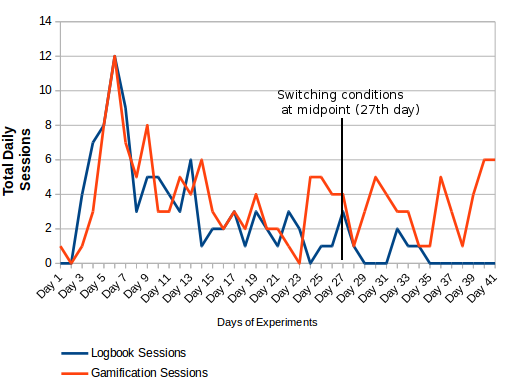
\includegraphics[width=0.6\textwidth]{Figures/scatter_daily_sessions.png}
    \rule{35em}{0.5pt}
  \caption{Total daily number of sessions from the two experimental conditions.}
  \label{figure:usagedailysessions}
\end{figure}
Findings on comparison of daily total number sessions summed from all users in each experimental condition showed that gamification had a significant total number of daily sessions compared to logbook as demonstrated by a non-parametric test called Mann-Whitney U Test on Table \ref{table:usagedays}. I made a decision to use the aforementioned test because the two independent samples were not distributed normally (From ``\emph{Shapiro-Wilk Normality Test}''\footnote{http://sdittami.altervista.org/shapirotest/ShapiroTest.html}). Also, Figure \ref{figure:usagedailysessions} shows trends on total daily sessions in between logbook and gamification conditions. This finding shows that there is a higher likelihood of a gamified system to be used more frequent compared to a logbook system.
\begin{table}[h!]
  \begin{center}
    \caption{Daily usage comparison between Logbook and Gamified systems for 41 days}
    \label{table:usagedays}
	\begin{tabular}{|L{3cm}|c|c|c|c|c|c|}
		\hline
		Groups&N&Rank Average&Sum Ranks&U&Z&P\\
		\hline
   		Daily logbook sessions&41&33.72&1701.5&\multirow{2}{*}{1159.5}&\multirow{2}{*}{-2.9538}& \multirow{2}{*}{0.00318}\\\cline{1-4} 
   		 		    Daily gamification sessions&41&49.28& 1701.5&&&\\
\hline
	\end{tabular}
  \end{center}
\end{table}
The pairwise usage comparison on number sessions between users on  two experimental conditions which excluded four pairs showed that the Log mean of number of sessions per day was significantly higher on gamification condition, M=0.459; SD=0.336, when compared to logbook condition, M=0.201 ;SD=0.196 with (t(9)= -2.6593 ; p= 0.0261 ; 95\% CI=  -0.477 to -0.039). The finding above suggests that there was an indication of a significant increase in frequency of daily usage when pairs where in gamification condition. The log mean is used in this case because the differences of logbook and gamification didn't have a normal distribution shape. Therefore, I performed transformation using a natural logarithm equation and after transformations on the original data, the differences of the new data on logbook and gamification had a normal distribution shape.

The utilization of different self-monitoring functionality on Figure \ref{figure:self_monitoring_usage}. showed that usage of some of the main self-monitoring features for steps and diet is lower in gamification compared to when in logbook condition. An explanation to this is that during  gamification condition users divided there attention between main logbook and virtual rewards. However, the trend in recording of diet/meals continued to remain the same between the two experimental conditions as the process of recording meals played an important role in earning some of the virtual rewards, therefore, intermediary users had to continue using that feature while in gamification condition. Figure \ref{figure:clicks_distr} shows the distribution of clicks among feedback features of the "Gamified Wellness App" and "The Logbook App".
\begin{figure}[htbp]
  \centering
    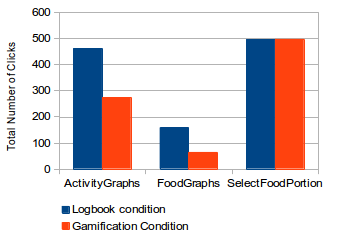
\includegraphics[width=0.6\textwidth]{Figures/self_monitoring_usage.png}
    \rule{35em}{0.5pt}
  \caption{Total clicks on feedback features for self-monitoring of wellness: ``Logbook App'' versus ``Gamified App''.}
  \label{figure:self_monitoring_usage}
\end{figure}
\begin{figure}[htbp]
  \centering
    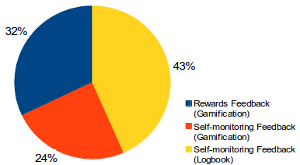
\includegraphics[width=0.45\textwidth]{Figures/clicks_distr.png}
    \rule{35em}{0.5pt}
  \caption{Total clicks on feedback features in the two experimental conditions : self-monitoring features versus rewards features.}
  \label{figure:clicks_distr}
\end{figure}
From Figure \ref{figure:clicks_distr}, we can see that gamification condition's clicks on feedback features are distributed between the main self-monitoring and virtual rewards features. The number of clicks on the main self-monitoring feedback features had decreased as users became interested to feedbacks provided by virtual rewards features more than the main self-monitoring features.

From Figure \ref{figure:usagedailysessions} above the trend shows the drop on Logbook condition as users who had been exposed to gamification condition before logbook condition became less interested with the "Logbook App" after being switched to it. The baseline data  can explain this usage information using descriptive trends since they were not statistically sufficient to explain the above usage. The drop in the total number of logbook sessions appears slightly the same in both younger and older intermediaries as shown on Figure \ref{figure:logbookbyage}.  But contrary to this is that younger intermediaries had slightly higher average on total number of sessions compared to the older ones while in gamification condition  as shown on Figure \ref{figure:gambyage}. Also on the average of total number sessions in both experimental conditions, the trend on average shows that younger intermediaries to have more sessions in overall as shown on Figure as more sessions were from gamification condition.  The term olerd and younger are defined by the age \textgreater= and \textless median age (15.5 years old) respectively.  Although the total number of sessions is relative to the number of days in which a pair of users had a particular experimental condition available to them, but younger and older intermediaries were evenly distributed to both experimental sequences (LG and GL groups). This means young and old intermediaries were both present in almost the same number in both experimental sequences hence their differences in number sessions which  is influenced by the number of days (27 days in phase 1 and 14 days in phase 2) are expected to cancel each other. The distribution by age group is presented on Table \ref{table:agregroupsall}.
\begin{figure}[htbp]
  \centering
    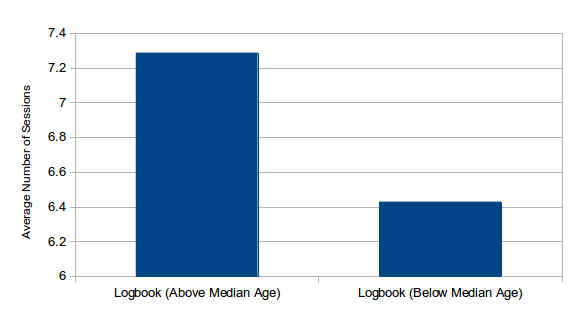
\includegraphics[width=0.5\textwidth]{Figures/logbookbyage.png}
    \rule{35em}{0.5pt}
  \caption{Average number of logbook sessions on  14 intermediaries: Age \textgreater= median age(=15.5) versus Age \textless median age.}
  \label{figure:logbookbyage}
\end{figure}

\begin{figure}[htbp]
  \centering
    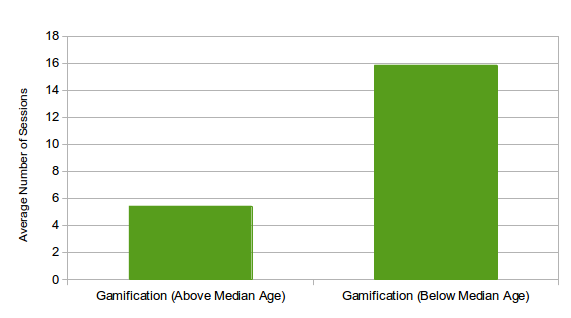
\includegraphics[width=0.5\textwidth]{Figures/gambyage.png}
    \rule{35em}{0.5pt}
  \caption{Average number of gamification sessions on  14 intermediaries: Age \textgreater= median age(=15.5) versus Age \textless median age.}
  \label{figure:gambyage}
\end{figure}

\begin{figure}[htbp]
  \centering
    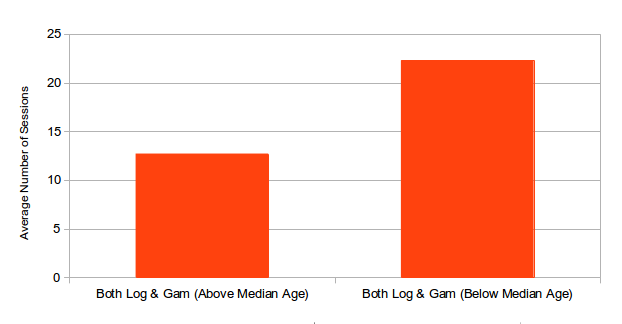
\includegraphics[width=0.5\textwidth]{Figures/bothexpebyage.png}
    \rule{35em}{0.5pt}
  \caption{Average of total number of sessions of  14 intermediaries on both experimental conditions: Age \textgreater= median age(=15.5) versus Age \textless median.}
  \label{figure:bothexpebyage}
\end{figure}
\begin{table}[h!]
  \begin{center}
    \caption{Age groups of intermediary participants}
    \label{table:agregroupsall}
	\begin{tabular}{|c|L{3.2cm}|L{1cm}|L{2cm}|L{2cm}|L{1.6cm}|L{1.3cm}|}
    		\hline
         &\textbf{Age Groups}&\textbf{Total users}&\textbf{No. of GL sequence}&\textbf{No. of LG sequence}&\textbf{No. of Females}&\textbf{No. of Males}\\
         \hline
         1&Age \textgreater=15.5 years&7&3&4&4&3\\  
\hline
         2&Age \textless15.5 years&7&4&3&3&4\\  
\hline
	\end{tabular}
  \end{center}
\end{table}
For pairs who had usage problems on Table \ref{table:usageproblems},three out of four intermediary users were above the median age and one below age. A different trend that excludes the intermediary users that belong in these four pairs still appears to be similar to Figures \ref{figure:logbookbyage} and \ref{figure:gambyage}. For logbook condition, only intermediary users from Pairs A, B were removed as their participation as they terminated their early before switched to logbook condition. Pairs C and D started with Logbook and they participated through logbook conditions despite problems in Pair C since the beginning of experiments. Therefore, the new logbook trend only excluded pairs A, and B (Figures \ref{figure:logbookbyage_mod}). For the gamification condition, we removed pairs A,B,C, and D, as usage problems affected their ability to continue engaging with the app, therefore the new trend on average sessions is shown on Figure \ref{figure:gambyage_mod}.

\begin{figure}[htbp]
  \centering
    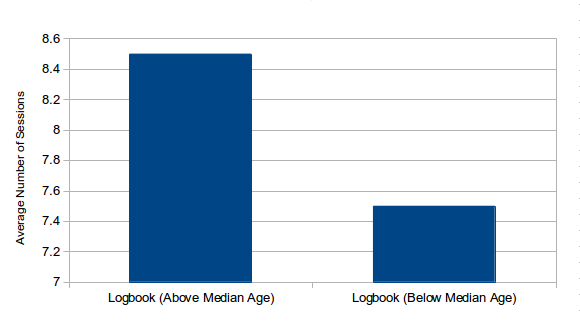
\includegraphics[width=0.5\textwidth]{Figures/logbookbyage_mod.png}
    \rule{35em}{0.5pt}
  \caption{Average number of logbook sessions on  12 intermediaries: Age \textgreater= median age(=15.5) versus Age \textless median age.}
  \label{figure:logbookbyage_mod}
\end{figure}
\begin{figure}[htbp]
  \centering
    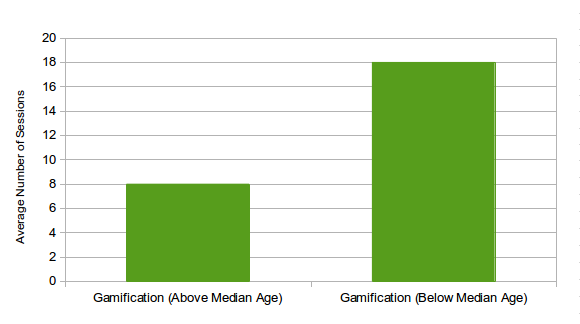
\includegraphics[width=0.5\textwidth]{Figures/gambyage_mod.png}
    \rule{35em}{0.5pt}
  \caption{Average number of gamification sessions on  10 intermediaries: Age \textgreater= median age(=15.5) versus Age \textless median age.}
  \label{figure:gambyage_mod}
\end{figure}
The same trends continue to hold as younger intermediaries appear to have higher average number sessions in gamification condition and lower average number of sessions in logbook condition. Koivisto and Hamari \cite{koivisto2014demographic} found that the usage of  a gamified system is highly affected by the novelty effect which is inversely proportional to the age of participants, meaning that highly usage due to the novelty effect may be reported in much younger participants.

The next trend is just looking at usage with respect to both ages of beneficiaries and intermediaries.  If we consider all beneficiary users from all fourteen pairs then the trend on average number of sessions is as shown on Figure \ref{figure:pairs_usage_sessions}. The median age for intermediaries was 15.5 years old while the median age for beneficiaries was 44 years old. Therefore an individual participant belongs to either younger or older group depending on whether ones age is below or above their respective median age. Pairs with a combination of a younger intermediary, and younger beneficiary appears to have more sessions in average. Most of these sessions were contributed by gamification.
 
\begin{figure}[htbp]
  \centering
    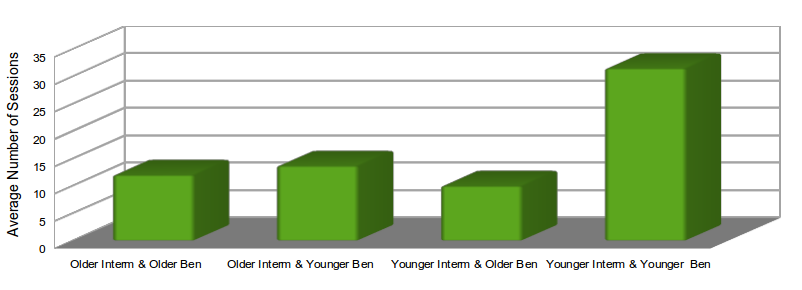
\includegraphics[width=0.6\textwidth]{Figures/pairs_usage_sessions.png}
    \rule{35em}{0.5pt}
  \caption{Average number of sessions on  14 pairs by age groups: intermediaries and beneficiaries}
  \label{figure:pairs_usage_sessions}
\end{figure}
On the next sub sections, user experiences of both intermediaries and beneficiaries are reported.
\subsection{Intermediaries' User Experience}
Most of the time, beneficiaries' usage of the app was facilitated by intermediaries in proximate enabling and proximate translation. These types of intermediated interactions have been discussed in the work by Sambasivan et al.\cite{sambasivan2010}. Baseline data indicated that interest of intermediary participants in using cellphones was higher than that beneficiary participants. For instance, in overall IMI scores to use cellphone, intermediaries (M=5.76, S.D= 0.41, N=14) scored  significantly higher than beneficiary participants (M=5.06, S.D= 0.71, N=13) with (t(25)= 3.1764, p=0.0039, 95\% CI = 0.2472 to 1.1589).

In user experience of intermediaries, the first finding is on how baseline intrinsic motivation and  demographic information such as age of intermediary users influenced user experience. From Figure \ref{figure:bothexpebyage} above, young intermediaries (age\textless median=15.5 years) appeared to had more number of sessions per day on average, but contrary to this trend was that, at baseline the average perceived enjoyment on helping with cellphone related tasks was higher in intermediaries with age\textgreater=median compared to intermediaries with age\textless median for the 12 intermediary users as shown on Figure \ref{figure:PE_HELP_Age}. 
\begin{figure}[htbp]
  \centering
    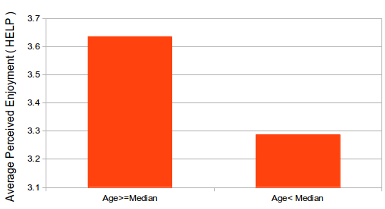
\includegraphics[width=0.5\textwidth]{Figures/PE_HELP_Age.png}
    \rule{35em}{0.5pt}
  \caption{Intermediaries' average perceived enjoyment to help others with cellphone tasks versus age group.}
  \label{figure:PE_HELP_Age}
\end{figure}
The descriptive finding on perceived enjoyment to use the family wellness app by age at midline and endline for the 12 intermediary users (excluding users from pairs A and B since they terminated their usage too soon) showed that the averages are higher on the intermediaries with age \textless median for both midline and endline points (Figure \ref{figure:PE_Interm_App}). If we split the two age groups by, participants with different characteristics are evenly present to both groups as shown on Table \ref{table:agegroups}. Therefore, comparison of trends by age groups in not much influenced by other factors such the experimental sequence of which participants were assigned to or gender. 
\begin{figure}[htbp]
  \centering
    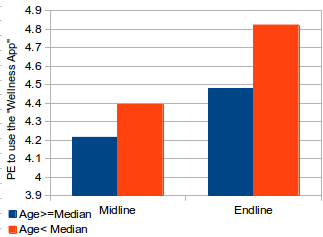
\includegraphics[width=0.5\textwidth]{Figures/PE_Interm_App.png}
    \rule{35em}{0.5pt}
  \caption{Intermediaries' average perceived enjoyment in using the app versus age group.}
  \label{figure:PE_Interm_App}
\end{figure}

\begin{table}[h!]
  \begin{center}
    \caption{Age groups of intermediary participants}
    \label{table:agegroups}
	\begin{tabular}{|c|L{3.2cm}|L{1cm}|L{2cm}|L{2cm}|L{1.6cm}|L{1.3cm}|}
    		\hline
         &\textbf{Age Groups}&\textbf{Total users}&\textbf{No. of GL sequence}&\textbf{No. of LG sequence}&\textbf{No. of Females}&\textbf{No. of Males}\\
         \hline
         1&Age \textless 15.5 years&6&3&3&2&4\\  
\hline
         2&Age \textgreater=15.5 years&6&2&4&4&2\\  
\hline
	\end{tabular}
  \end{center}
\end{table}

The trend on average perceived enjoyment in both logbook and gamified conditions appeared to be slightly higher in younger intermediaries compared to older intermediaries as shown on Figure \ref{figure:PE_Interm_App_exp_seq}. 
\begin{figure}[htbp]
  \centering
    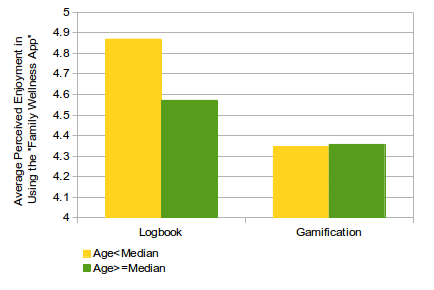
\includegraphics[width=0.5\textwidth]{Figures/PE_Interm_App_exp_seq.png}
    \rule{35em}{0.5pt}
  \caption{Intermediaries' average perceived enjoyment in using the app versus age group (Logbook and Gamification).}
  \label{figure:PE_Interm_App_exp_seq}
\end{figure}

Figures \ref{figure:PE_Interm_App} and \ref{figure:PE_Interm_App_exp_seq}  suggest that the task of helping was more interesting to younger intermediaries due to the existence of the aforementioned motivational affordances.

There several factors that influence intermediaries to use the app and these are:
\begin{enumerate}

\item{\textbf{The phone effect}}: The phenomenon of sharing phones was important in nurturing the relationship between intermediaries and beneficiaries. Parents were lending their phones to their kids to access social media sites and games. Having access to a phone while providing help to beneficiary participants can be viewed as one of the motivating factors to intermediary participants who didn't have smart-phones or data bundles in their smart-phones. Some intermediary participants had installed games, other apps on those phones.

\userquote{\textbf{Siyamthanda}, a female intermediary from Langa, 12 yrs old} {``I had freedom [in using the app] because sometimes she left the phone with me and I was able to play games''}

\userquote{\textbf{Aziza}, a female beneficiary from Athlone, 35 yrs old} {``We would fight over it[the app]. Because he always wants to be on the phone. Always always.''}

\userquote{\textbf{Likhaya}, a male intermediary from Langa, 16 yrs old} {``I didn't feel burdened. You know I also play games on the phone. [Implying he also played games with the phone during logbook condition therefore he didn't feel burdened to help his mother]''}

Therefore, a phone had some effect, since intermediaries were helping in return they have access to cellphone to access functionality or services they like.

\item{\textbf{Gamification comparison}}: The ``Gamified App'' was designed in such a way that a pair will earn rewards based on usage and the average number of steps walked by a beneficiary participant who is a member of the pair. The purpose of rewards was to foster users' intrinsic experiences such as competitiveness and a sense of autonomy which are predictors of intrinsic motivation. Rewards depended on four parameters and these were the number of steps walked by a beneficiary user, the number of days the app has been used by an intermediary to either to record meals or to view feedback on meals, points, steps, gardens, etc. 

Comparison on virtual rewards among intermediaries motivated intermediaries to check the app more often compared to when they were in logbook condition as highlighted on the aforementioned usage findings (sub section \ref{usageoutcome}). Intermediaries were competing which other on the leader board and they talked about their points whenever they meet face to face.

\userquote{\textbf{Jenner}, a female beneficiary from Athlone, 45 yrs old} {``He [Leon (her 15 years old son) ] likes this exercise (using the app) because among him and his friends, they would have that competition like `I got more points than you' and that motivated him to get interested with the app''} 

The competition also led intermediaries to work closer with their beneficiaries.

\userquote{\textbf{Kelvin}, a male intermediary from Athlone, 15 yrs old} {``When I see other people trying to come above me [on the leader board]. I hand over the phone to my mom so she can walk more steps.''} 

\userquote{\textbf{Celine}, a female intermediary from Athlone, 16 yrs old} {``I told my mom that me my self I want our team to have the highest points. Yes she said she is going to do that.''} 

\userquote{\textbf{Sophia}, a female intermediary from Athlone, 17 yrs old} {``Sometimes that person may be first so I tell my mom that we must also be at the first place.[She looks at the  leader board and she sees so and so is at first place there she talks to her mother that they should also aim for the first position] ''} 

\userquote{\textbf{Jenner}, a female beneficiary from Athlone, 45 yrs old} {``When he [Leon] looked through it [The app] and sees their points, he would say `Mom, we need to do something here, because look at their points and our points'. So it was quite interesting.''} 

There was a scenario of one pair of whereby not only the beneficiary was using the pedometer, an intermediary was also taking turns to use the pedometer, therefore they were collaborating in accumulating steps. Both an intermediary user and a beneficiary user had discussions of whether the person whose turn it was had walk enough steps. They did this to accumulate more steps than other pairs. In addition to comparison other intermediary users came to the app to the gamified app to connect to other users.

\userquote{\textbf{Celine}, an intermediary} {``I ask her how far did you walk?  She would say she walked very far. She tells me that I must have the phone to walk more steps. She would say `I got more more walking than you' [They were collaborating with her mother in accumulating steps]. She sometimes writes the steps on the page and she tells me yesterday I day I had more points than you [points referring to steps ]''} 

Rewards were specific for gamification condition by they appeared to also affected pairs that had started with logbook conditions as some intermediary users were pushing their beneficiaries to do more by expecting to get rewards once they are switched to gamification condition.

\userquote{\textbf{Kefiloe}, a female beneficiary from Langa, 26 years old} {``I think we talk more than before the family wellness app. Before the family wellness app, after work it was just ``Hi'' and then I go to my room but now. But now she would come to my room  and say let me see your phone,  what did you eat today,  and write everything down on the phone. So we are more closer than before because of this. Most of the time she used to say that `we must win this'''} 

\item{\textbf{Requests from beneficiary users}}: There were times where intermediary users engaged with the app only upon receiving requests from beneficiaries. In both absence and presence of gamification, intermediaries had to fulfil requests from beneficiaries.  But during logbook condition, intermediaries appeared to be less enthusiastic in handling those requests. Some beneficiaries complained that there were several incidences of where intermediaries were refusing to fulfil these requests and it happened more often during logbook condition. It was observed that in most of these cases, intermediary participants' autonomy was violated as requests came at times where intermediary participants were either studying for exams or doing something else and they felt it was not the right time to fulfil those requests. This made some of the intermediary participants to feel that their parents were nagging them. For instance, \textbf{Lunga}, a male intermediary participant from Langa, aged 17 years, felt annoyed when his mother insisted they should enter the family wellness app while he was busy using social media through the intervention's phone. This happened during logbook condition. Also a similar situation happened to \textbf{Jennifer}, female intermediary participants from Athlone, aged 18 years who also felt irritated by her mother's constant requests during logbook condition. In addition she felt the app was not that exciting as she said ``\emph{The app was okay first but it started to get boring. You don't want to go into it any more. I think there will be some excitement now if the game comes in. When do we get the game}''. She was curious to know when they will be switched to gamification because she thought the logbook condition was boring.

Interest of intermediaries or pairs in general varied as some exhibited interests on interacting with others through the app while others where focused on achievements (i.e. dominating others in competitions). Gamification appeared to be the most dominant factor that influenced usage as we have already seen that the frequency of usage showed a higher value in gamification when compared to logbook. 

\userquote{\textbf{Aziza}} {``We [with Kelvin] were not talking to others because all we wanted was to win. We didn't want them to know but they could see from the app''}
 
Only two intermediaries had tried to interact with others using social features of the app or comment on rewards from their peers. These are some of the comments that were shared by these participants.

\userquote{\textbf{Simon}, a male intermediary from Athlone, 15 yrs old} {``Fish are increasing neh.[He commented this on a fish tank owned by Kelvin and his mother]''} 

\userquote{\textbf{Siyamthanda}, a female } {``Wow it shows that you are working hard  Clara\#2.[She congratulated a female intermediary called Clara for being on the second position on Fish tanks.]''} 

However, not all intermediaries had a positive user experience on utilizing gamification, that is why the average perceived enjoyment appears to be lower for both age groups while in gamification condition compared to the logbook condition (Figure \ref{figure:PE_Interm_App_exp_seq}).

\end{enumerate} 

Leader-board can demotivate those users that are at the bottom but it can foster aspects of relatedness for all users\citep{sailer2013:psychological}. In this case there were users who never made any advancement in badges hence they appeared at the bottom of the leader board. Some participants it was due to technical problems as reported on Table \ref{table:usageproblems}. But there few exceptions of which two users had no technical problems but never had any advancement in badges despite their efforts in using the gamified system more than the logbook condition as shown on Figure \ref{figure:badge_failure_2}. One user was from the `LG' group (Keller), while the other one was from the `GL' group (Leon).  Their beneficiary participants were not walking enough steps despite the fact that these two intermediaries had put  more efforts in using the app during gamification condition than in logbook condition.
\begin{figure}[htbp]
  \centering
    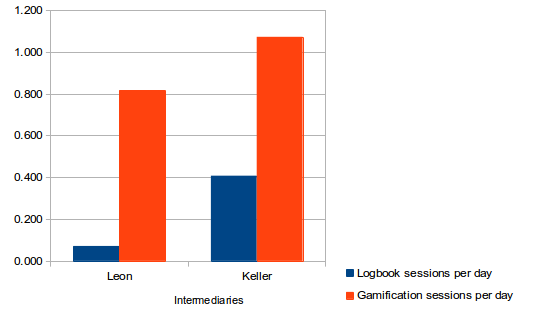
\includegraphics[width=0.7\textwidth]{Figures/badgesfailures2.png}
    \rule{35em}{0.5pt}
  \caption{Logbook Vs Gamification for two users that had no technical problems but never had any badge advancement.}
  \label{figure:badge_failure_2}
\end{figure}

Badges were earned in combination of both the app usage and average number of steps walked by a beneficiary user. One beneficiary who was working with one of these intermediary users also reported in interviews that there was always a contention with her intermediary when this beneficiary wanted to see what was going in the app as the intermediary was not voluntarily willing to help some of the time. It is hypothesized that this could be one of the factors that played a role in demotivating some participants during gamification condition. There were also cases of  where intermediaries doubted the credibility of the system because their peers appeared to be more engaged with the app, but were at lower positions on the leader board. 

\userquote{\textbf{Akhona}, a female intermediary from Langa, 16 yrs old} {``It [The experience in using the gamified app] was the same as last time (during logbook condition) except for the game part. I was actually above some of the others. That was weird. Because they were more interested in the app than me.''} 

On the aforementioned excerpt, \emph{Akhona} was referring to the two intermediaries from pairs C , and D that had usage problem (Table \ref{table:usageproblems}) as these two users used the app more in logbook condition, therefore, Akhona's anticipation was that they would be more competent than her but surprisingly she was ahead of them.  Therefore, even in perceived competence Akhona reported lower score in gamification compared to logbook despite using gamification for 7 out of 14 days and logbook for only 4 out of 27 days.

Therefore, in comparing the support for the three basic psychological needs, pairs that never had any advancement in badges were not considered on aspects of perceived competence and autonomy since majority of them appeared to have a lower perceived enjoyment in gamification when compared to logbook. Autonomy and competence are major predictors of perceived enjoyment. An assumption was that a negative experience was the result of failure of the gamification design to match challenges with abilities. i.e. efforts of beneficiaries differed hence challenges should have matched with individual abilities of beneficiaries within pairs. When challenges are too difficult as they don't match users' skills, end users can become demotivated \citep{zhang2008motivational}. In addition, some of those that had technical problems, their problems were so severe to the extent that they were unable to participate fairly in gamification condition. A total of five intermediary users never had any advancement in badges, therefore, they were excluded in the analysis of motivation of which three are from those that had technical problems (Pairs A, C and D on Table) and two, they had dome more efforts in using the gamified system but there less steps detected from their beneficiaries. As result only nine intermediary users were considered in the perceived competence, and perceived autonomy.

On the aspect of relatedness, all intermediaries were considered because all of them had directly or indirectly use at least one of relatedness features such as receiving SMS showing which teams have advanced in badges, viewing a leader board that shows teams' points, viewing gardens or tanks of different people, and display of badges from each team. These are some of mechanisms to support an aspect of relatedness\citep{sailer2013:psychological}. But in additional, there are intermediary users who knew each other before, and they talked about thinks on the app such as steps comparisons. However there are this that interfered with experiments.     
  
The findings (Table \ref{table:imiwellnessinterm}) indicate that perceived competence of intermediaries in using the ``Family Wellness App'' was significantly higher in the gamified condition than in the logbook condition in the nine intermediaries that were analysed. Perceived autonomy and perceived relatedness were all not different between gamification condition and logbook condition. When I compared perceived autonomy during phase 1 of experiments (at midline point) and during phase 2 of experiments (endline), thehttp://www.kat.ph/ perceived autonomy was significantly higher at midline (M=4.44; S.D=0.93) than at endline (M=3.89; S.D=0.76), (t(8)= 2.5298; p=0.0353; 95\% CI= 0.049 to 1.062). Several reasons contributed to this, and these include (1)the learning effect as users became used to the application and the whole exercise was not exciting any more, and (2) most intermediaries were writing exams, and felt that they had no time to do the app, although their beneficiaries kept on pushing them to do the app.

\begin{table}[h!]
  \begin{center}
    \caption{Comparison of ten intermediaries' scores on sub-scales of competence, autonomy, enjoyment, and relatedness in using the ``Family Wellness App}
    \label{table:imiwellnessinterm}
	\begin{tabular}{|c|c|c|}
		\hline
		Mean &Logbook App&Gamified App\\
		\hline
		 \multirow{2}{*}{Perceived competence}&M=5.42; SD=0.88&M=6.03; SD=0.65\\\cline{2-3} 

		 &\multicolumn{2}{|l|}{t(8)=3.1418; p=0.0138 ; 95\% CI= -1.0712 to -0.1643 } \\
\hline
		 \multirow{2}{*}{Perceived autonomy}&M=4.0; SD=0.92&M=4.33; SD=0.84\\\cline{2-3} 

		 &\multicolumn{2}{|l|}{t(8)= 1.2344; p= 0.2521; 95\% CI=  -0.956 to 0.289 } \\
\hline
		 \multirow{2}{*}{Perceived relatedness}&M=4.20; SD=0.59&M=4.5; SD=1.04\\\cline{2-3} 
		 &\multicolumn{2}{|l|}{t(13)= 1.5046; p=0.1563; 95\% CI= -0.725 to 0.13 } \\
\hline
	\end{tabular}
  \end{center}
\end{table}
\subsection{User Experience of Beneficiaries}
As most beneficiaries only interfaced with the app through intermediary users, beneficiaries' user experience relied on cooperation they got from intermediaries. On support for the three basic psychological needs, there was no difference between logbook and gamification. However, aspects of relatedness (N=14) appeared to improve significantly with time when compared between midline (M=4.43; S.D=0.92) and endline (M=5.38; S.D=1.08) with (t(13)= 2.3736; p= 0.0337; 95 \% CI=-1.819 to -0.0855 ). Therefore, the intervention in general made beneficiaries felt more closer at end-line.

On utilizing the app through intermediaries, there are cases where beneficiaries had a negative experience as result of intermediaries refusing to assist upon being given requests. This happened in cases of where intermediary users didn't feel like helping because of being occupies by other tasks such as reading for exams or because they felt the app was boring especially in logbook condition. Younger beneficiaries had a tendency of being keen to compete with others. But for older intermediaries, interests what happening in gamification In addition to that, from Figure \ref{figure:pairs_usage_sessions}, a combination of younger intermediary and beneficiary users had more sessions in average and this is because gamification influenced younger intermediary users to use the app, while it also influenced younger beneficiaries to pass their requests to their respective intermediaries more often. For instance in interviewing one pair that consisted of a younger intermediary and beneficiary users, this pair had highest number of sessions in gamification. In the course of using the app they both exhibited playfulness behaviours in engaging with gamification of whereby they discussed strategies about beating other teams. So every time a beneficiary user from this pair would request her intermediary to open the app so that she can see if they are ahead of other teams.

In the next sub-section, the IMIs in self-monitoring of diet and activity are reported. Four pairs with usage problems (Table \ref{table:usageproblems}) were excluded.
\subsubsection{IMI in Self-Monitoring of Diet}
The results on self-monitoring of diet (baseline, midline, and endline) are shown on Table  \ref{table:imidietbenf}. The Mauchly’s test indicated that the assumption of sphericity was not violated with  $\chi{}$\SP{2}(2)=3.76, p=0.152. The results (N=10) on  ``Self-monitoring of Diet'' shown on Table \ref{table:imidietbenf} were from ``Sphericity Assumed'' output. ANOVA showed that there was a significant difference of average IMI scores on self-monitoring of diet measured at baseline, midline and endline.
\begin{table}[h!]
  \begin{center}
    \caption{Comparison of ten beneficiaries' IMI scores in self-monitoring of diet at baseline, midline and endline}
    \label{table:imidietbenf}
	\begin{tabular}{|L{2.8cm}|L{3.2cm}|L{3.2cm}|L{3.2cm}|}
		\hline
		Mean IMI Score &Baseline&Midline&Endline\\
		\hline
		 %\multirow{3}{*}
		 {Self-monitoring}&M=4.48; SD=1.24&M=5.07; SD=1.19;&M=5.55; SD=0.95\\\cline{2-4} 

		of Diet &\multicolumn{3}{|l|}{F(2,18)=3.787; p=0.042} \\
\hline	\end{tabular}
  \end{center}
\end{table}
A finding from a pairwise comparisons (a paired student t-test) indicated that the IMI score at endline was significantly higher than at baseline (Table \ref{table:imipairwisediet}). There was no significant difference on baseline versus midline and midline versus endline (Tables \ref{table:imipairwisediet1}, and \ref{table:imipairwisediet2}). Motivation to self-monitor diet appeared to increase with time as shown on Figure \ref{figure:imi_diet}. The interpretation of the above findings are that the wellness app appeared to had a significant effect of time on motivation of beneficiaries to self-monitor their diet.
\begin{table}[h!]
  \begin{center}
    \caption{Pairwise comparisons of IMI scores in self-monitoring of diet: Baseline versus Midline}
    \label{table:imipairwisediet}
	\begin{tabular}{|L{2cm}|L{4cm}|L{4cm}|}
		\hline
		Mean &Baseline&Midline\\
		\hline
		 \multirow{2}{*}{IMI Score}&M=4.48; SD=1.24&M=5.07; SD=1.19\\\cline{2-3} 

		 &\multicolumn{2}{|l|}{t(9)=-1.298; p=0.227 ; 95\% CI= -1.621 to 0.439} \\
\hline
	\end{tabular}
  \end{center}
\end{table}
\begin{table}[h!]
  \begin{center}
    \caption{Pairwise comparisons of IMI scores in self-monitoring of diet: Baseline versus Endline}
    \label{table:imipairwisediet1}
	\begin{tabular}{|L{2cm}|L{4cm}|L{4cm}|}
		\hline
		Mean &Baseline&Endline\\
		\hline
		 \multirow{2}{*}{IMI Score}&M=4.48; SD=1.24&M=5.55; SD=0.95\\\cline{2-3} 

		 &\multicolumn{2}{|l|}{t(9)=-2.457; p=0.036 ; 95\% CI= -2.06083 to -0.08517} \\
\hline
	\end{tabular}
  \end{center}
\end{table}
\begin{table}[h!]
  \begin{center}
    \caption{Pairwise comparisons of IMI scores in self-monitoring of diet: Midline versus Endline}
    \label{table:imipairwisediet2}
	\begin{tabular}{|L{2cm}|L{4cm}|L{4cm}|}
		\hline
		Mean &Midline&Endline\\
		\hline
		 \multirow{2}{*}{IMI Score}&M=5.07; SD=1.19&M=5.55; SD=0.95\\\cline{2-3} 

		 &\multicolumn{2}{|l|}{t(9)=-1.975; p=0.08 ; 95\% CI= -1.0342 to 0.07017} \\
\hline
	\end{tabular}
  \end{center}
\end{table}

\begin{figure}[htbp]
  \centering
    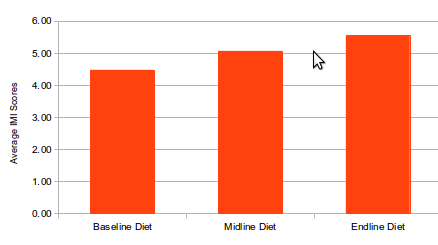
\includegraphics[width=0.4\textwidth]{Figures/imi_diet.png}
    \rule{35em}{0.5pt}
  \caption{Trend on Average IMI Scores of Self-Monitoring of Diet at Baseline, Midline, and Endline.}
  \label{figure:imi_diet}
\end{figure}
The aforementioned ANOVA finding on comparison among baseline, midline, and endline doesn't discern between different experimental conditions of which pairs of users were exposed to. The ANOVA finding (N=10)(Table  \ref{table:imidietbenf2}) on the comparison of IMI scores to self-monitor diet, among baseline, logbook, and gamification conditions showed that there was no significant difference of average IMI scores on self-monitoring of diet measured during baseline, logbook and gamification conditions. This finding is from the ``Sphericity Assumed'' output of the ANOVA test since the Mauchly’s test indicated that the assumption of sphericity was not violated with  $\chi{}$\SP{2}(2)=2.19, p=0.335. The trend on averages shows both logbook and gamification to be slightly higher than baseline as shown on Figure \ref{figure:imi_diet2}. The conclusion from this finding is that both versions of the prototype have shown an indication of increasing motivation of beneficiaries to self-monitor diet.
\begin{table}[h!]
  \begin{center}
    \caption{Comparison of ten beneficiaries' IMI scores in self-monitoring of diet at baseline, after logbook, and  after gamification conditions}
    \label{table:imidietbenf2}
	\begin{tabular}{|L{2.8cm}|L{2.5cm}|L{2.5cm}|L{2.5cm}|}
		\hline
		Mean IMI Score &Baseline&Logbook&Gamification\\
		\hline
		 %\multirow{3}{*}
		 Self-monitoring&M=4.48; SD=1.241&M=5.28; SD=1.05&M=5.34; SD=1.16\\\cline{2-4} 
		 of Diet&\multicolumn{3}{|l|}{F(2,18)=3.787; p=0.087} \\
\hline	\end{tabular}
  \end{center}
\end{table}
\begin{figure}[htbp]
  \centering
    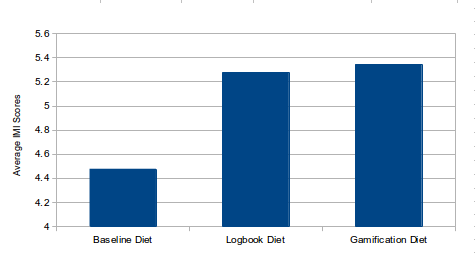
\includegraphics[width=0.4\textwidth]{Figures/imi_diet2.png}
    \rule{35em}{0.5pt}
  \caption{Trend on Average IMI Scores of Self-Monitoring of Diet at Baseline, Logbook, and Gamification.}
  \label{figure:imi_diet2}
\end{figure}
\subsubsection{IMI in Self-Monitoring of Activity}
The results (N=9) on self-monitoring of activity are shown on Table  \ref{table:imiactivitybenf}. The results are based on a sample of nine beneficiary users as one participant didn't complete this part of the questionnaire at baseline.  The Mauchly’s test indicated that the assumption of sphericity was violated with  $\chi{}$\SP{2}(2)=8.248, p=0.016. The value $\epsilon$ on Greenhouse Geisser was ``\textless 0.75'', therefore, the results on  ``Self-monitoring of Diet'' shown on Table \ref{table:imiactivitybenf} were selected from ``Greenhouse-Geisser'' output. ANOVA showed that there was no significant difference of average IMI scores on self-monitoring of activity measured at baseline, midline and endline. The trend of means appears to increase from baseline to endline as shown on Figure \ref{figure:imi_activity}.

There are several factors that could have contributed to results not being significant among baseline, midline,endline points,. The first hypothesized reason is tracking of physical activity appeared to be easy in majority of the participants even without tracking devices as people can estimate the distance they walk daily and they consider this as tracking even though they might have means to record this information, hence their motivation was high at baseline unlike diet self-monitoring which they consider it to be cumbersome due to external barriers such as health food being expensive, therefore at baseline participants felt more motivated to track their activity. The second hypothesized reason is that the sample size was small hence there was a smaller power in detecting significant difference. But we have seen that the trend in motivation increases with time.
\begin{table}[h!]
  \begin{center}
    \caption{Comparison of ten beneficiaries' IMI scores in self-monitoring of activity at baseline, midline and endline}
    \label{table:imiactivitybenf}
	\begin{tabular}{|L{2.8cm}|L{2.5cm}|L{2.5cm}|L{2.5cm}|}
		\hline
		Mean IMI Score &Baseline&Midline&Endline\\
		\hline
		 %\multirow{3}{*}
		 Self-monitoring&M=4.82; SD=1.002&M=5.28; SD=1.003&M=5.41; SD=0.894\\\cline{2-4} 
		 of activity&\multicolumn{3}{|l|}{F(1.182, 9.455)=2.936; p=0.116} \\
\hline	\end{tabular}
  \end{center}
\end{table}

\begin{figure}[htbp]
  \centering
    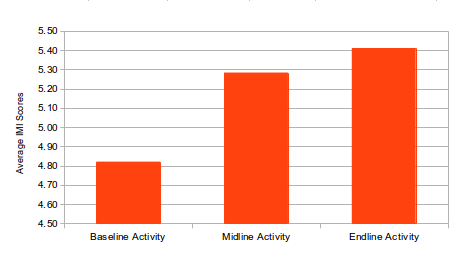
\includegraphics[width=0.4\textwidth]{Figures/imi_activity.png}
    \rule{35em}{0.5pt}
  \caption{Trend on Average IMI Scores of Self-Monitoring of Activity at Baseline, Logbook, and Gamification.}
  \label{figure:imi_activity}
\end{figure}
The finding from an analysis (N=9) that examined if there is a difference among baseline,logbook, and gamification in self-monitoring of activity, showed that there was no significant difference of average IMI scores on self-monitoring of activity measured at baseline, logbook and gamification (Table {table:imiactivity2benf}). The Mauchly’s test indicated that the assumption of sphericity was violated with  $\chi{}$\SP{2}(2)=6.788, p =0.034. The value of $\epsilon$ on Greenhouse Geisser was ``\textless 0.75'', therefore, these results on  ``Self-monitoring of Activity'' were selected from ``Greenhouse-Geisser'' output of oen way with repeated measures ANOVA test. The trend in motivation increases in both logbook and gamification compared to baseline as shown on Figure \ref{figure:imi_activity2}
%epsilon=0.617
\begin{table}[h!]
  \begin{center}
    \caption{Comparison of ten beneficiaries' IMI scores in self-monitoring of activity at baseline, logbook and gamification}
    \label{table:imiactivity2benf}
	\begin{tabular}{|L{2.8cm}|L{2.5cm}|L{2.5cm}|L{2.5cm}|}
		\hline
		Mean IMI Score &Baseline&Logbook&Gamification\\
		\hline
		 %\multirow{3}{*}
		 Self-monitoring&M=4.82; SD=1.002&M=5.33; SD=0.9762&M=5.37; SD=0.9276\\\cline{2-4} 
		 of activity&\multicolumn{3}{|l|}{F(1.234, 9.872)=2.783; p=0.123} \\
\hline	\end{tabular}
  \end{center}
\end{table}
\begin{figure}[htbp]
  \centering
    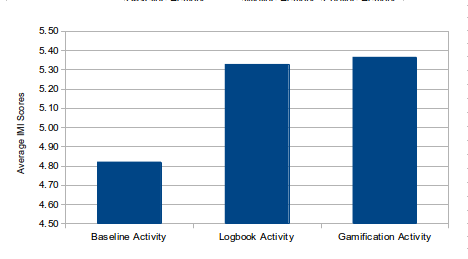
\includegraphics[width=0.4\textwidth]{Figures/imi_activity2.png}
    \rule{35em}{0.5pt}
  \caption{Trend on Average IMI Scores of Self-Monitoring of Activity at Baseline, Logbook, and Gamification.}
  \label{figure:imi_activity2}
\end{figure}
\section{Discussion}
In many cases, usage of the app was controlled by intermediaries. Intermediaries engaged with the app mostly because of two factors and these were: either competitions with others or request from their beneficiaries. Beneficiaries interests varied and it was influenced by  either one of the following factors or both: (1) leader board; and (2) instrumental value provided by the app. Not all beneficiaries were motivated by gamification. However, gamification was the main source of motivation to intermediaries and it played a pivotal role in mediating usage. Gamification also mediated intermediaries to influence or persuade their beneficiaries.  For instance, in one scenario a beneficiary described how serious her son was engaged in competition with others and was always reminding her to carry the pedometer whenever she wants to go out as shown on the following excerpt.

\userquote{\textbf{Jenner}, a female beneficiary from Athlone, 45 yrs old} {``Sometimes may be I forget to take the phone when I go walking and he would ask me `did you take the phone with you' Ooh Gosh I forgot.  Because when I walk to Park Town to exercise and sometimes  I am in such a hurry I forget the phone, he will be crossed with me. ''} 

For intermediaries that started with logbook, majority of those that engaged with logbook many times did with an interest of winning the competition once switched to gamification. Therefore, this affected the separation of experimental as users were aware that they will be switched to gamification at some point. For the case of perceived competence, the difference between logbook and gamification was statistically significant and intermediary user in gamification felt more competent.Statistical significance in difference was not achieved in cases of autonomy and relatedness due to the learning effect and a smaller sample size. 

Apart from gamification, another important source of motivation that can be leveraged is, beneficiaries' phones. Beneficiaries were custodians of intervention's phone. But in many cases when beneficiaries were at home they left the phone with the intermediaries who were interested with social media sites and  games. Intermediaries were interested with those phones because of either of the two reasons or both: (1) Interventions phone's were better than intermediaries' phones or intermediaries didn't have smart phones that can enable to access services they desire; and (2) Availability of data bundles in intervention's phones through inserted SIM cards. In these scenarios, some intermediaries were implicitly reciprocating the favours of having freedom to use the phone by serving requests from their beneficiaries. In the context of ICTD, non-prescribed use of devices or other technologies allocated for an intervention is considered to be an aspect of play which is a capability as it fosters motivation to participate in an intervention \citep{ferrplay2015}. Therefore, one can capitalize on this motivation introduced as the result of sharing phones and it can be viewed as part of motivational affordances to encourage ongoing use of a system through young intermediaries within family settings. Utilization of the motivational effect of the phone in mediating such an intervention depends on interest of beneficiaries on the intervention. Without requests from beneficiaries, and with absence gamification on the app for intermediaries, the phone effect itself cannot mediate usage of the app unless it goes in parallel with those two mediating factors for usage.

Gamification was the most dominating motivational affordance. However, there are some factors that need to be taken into considerations in design of gamification in order to curb negative experiences which appeared to harm intrinsic motivation of some intermediary users. Awarding virtual rewards to intermediary users based on partial efforts from beneficiary participants seemed not to resonate with the notion of matching challenges to skills of the main users. For instance in awarding badges there were two conditions to be met. The first condition was that the app has to be used for a certain minimum number of days as specified by requirements of a specific badge. The second condition was that, an average number of steps that have been walked so far has to be not below a certain threshold for that specified badge. It became impossible for some intermediary users to move from one badge to the next because efforts by beneficiary users differed and this may impacted motivation of intermediary participants and this harmed their intrinsic motivation. When challenges are too difficult as they don't match users' skills, end users can become demotivated \citep{zhang2008motivational}. 

Another shortcoming observed in the app, is that the gamified system didn't give users much autonomy apart from only configuration of avatars and editing of profiles. For instance, freedom to select the level of gamification appropriate to the skills they possess at a particular moment was not supported in the app. Examples of ways on which autonomy is supported include profiles, avatars, macros,configurable interface, alternative activities, privacy control, etc. \citep{francisco2012analysis}. 

One of the approaches that could be used to minimize the effect of the  aforementioned shortcomings is to give users more autonomy to select different levels of gamification they want to participate. There could be levels such as beginners, intermediate, advanced, etc. Pairs that are on the same level could be grouped together and not mixed with pairs with levels that are different. In addition, users could be allowed to select which features they would like to include in their interfaces from a range of features such as chat rooms, leader-boards, botanical gardens etc. More autonomy can also be given in customization of privacy in terms of whether they would like to share their information or not. Customization of avatars is also important because It was observed that most users changed their avatars during gamification and one user explained that she sees the avatar she selected as a representation of herself. Through avatars, these users embodied their identities.
 
A different approach in increasing engagement of intermediary users is  to allow intermediary participants to benefit from the app information, by incorporating their wellness data i.e. steps. The former can also be combined with the latter. There were some observed scenarios that support the utilization of the latter approach. For instance, there was one pair of whereby not only the beneficiary participant was using the pedometer as an intermediary was also using it. They were taking turns to use the pedometer, therefore, they were collaborating in accumulating steps. This pair had discussions of whether the person whose turn it was had walked enough steps. The goal was to accumulate more steps than other pairs. A different scenario is whereby intermediaries claimed to also be benefiting from nutrition/diet information since the same type of meal is shared at home, therefore, if beneficiary participants ate something that is not healthy while at home then there is a likelihood of an intermediary participant to have eaten the same type of meal too.
\begin{flushright}
\end{flushright}


% Chapter 1

\chapter{Overall Discussion} % Main chapter title

\label{discussionchapter} % For referencing the chapter elsewhere, use \ref{Chapter1} 

\lhead{Chapter \emph{Overall Discussion}} % This is for the header on each page - perhaps a shortened title

%----------------------------------------------------------------------------------------
The main research questions were centred around factors that may affect utilization of a personal health informatics through intermediaries, and also the effectiveness of gamification in increasing engagement of intermediaries. The most prominent factors are social relationships, support for the two sets of users to achieve an optimal flow, and  different requirements for motivation strategies for users from each set. On the effectiveness of gamification, it has demonstrated a potential too increase frequency of usage through intermediaries even though it has some challenges and limitation that need to be addressed.
  
In this chapter, the focus of discussion is on design considerations for the overall intervention. These design considerations include some of the aforementioned social factors that may contribute to the success of the intervention, and approaches that can be utilized in order to keep both intermediaries and beneficiaries engaged with a personal health informatics system.
 
\section{Leverage Family Settings}
Informative evaluations revealed that involving children who are family members is the key to success of this intervention. This idea of collaborative interfaces for health information within family settings has been explored in computer supported collaborative work (CSCW) literature. \cite{colineau2011motivating} designed a system to support a family to select a collective health goal and receive feedbacks that entailed comparisons between families. Their system was found to encourage members from within a family or members of different families, to work together and in particular to help each other in finding ways to live a healthily lifestyle. 

Family settings provide an idyllic opportunity for members to discuss healthy issues collaboratively. Collaboration between a parent and a child or close family members had a positive impact on child's perception as some intermediaries shared testimonies about their habituation of skills on eating healthy. In addition, intermediaries in some cases logged their data about meals because what they ate was not different from what had been eaten by their respective beneficiaries. A study by~\cite{grimes2009toward} identified four key areas of consideration in which sharing of, and reflection on, health information can be leveraged within family context as follows: (1) overlaps of routines between family members through shared meals, space, etc which can provide opportunities for collaborative data logging and reflection among family members; (2) sharing is done at the expense of balancing competing values of openness, caring, and modelling with the value of protection; (3) understanding of sensitivity on comparisons and competition based upon health information in the context of the family as it may have negative consequences; and (4) collaborative sharing of, reflecting on, health information can also foster family's bond. In the context of this research, it was evident that the app had increased the bond between participating family members as majority of them claimed that were interacting more often. This is also demonstrated by playfulness behaviours that were exhibited in the process of sharing information as it was shown in one of the excerpt in chapter \ref{prototytpe2chapter} (Evaluation of Prototype II):

\userquote{\textbf{Zandiwe}, a beneficiary} {` When she got time, when she is done with her homework she comes and sees the app. And then laughs at me like `Yo yo yo [An interjection for Xhosa speakers to express the feeling of amazement by something] you can walk yo yo yo', like `you walked a lot today' and what what [She was implying to other words said by Lindiwe]''}

In existing work from computer supported collaborative work it appears the emphasis is on parents trying to model health behaviors of their children.  For a instance in a study by ~\cite{saksono2015spaceship}, a collaborative exergame was developed in order to support both parents and kids to exercise together. Although their goal was to help kids learn from their parents, the collaborative environment was beneficial to both parents and children.

In our case it was peculiar that children were attempting to nudge their parents to live healthily. Therefore, it not only about the parent guiding the child also the child can become a facilitator for guiding the parent about health choices. This was mediated by an existing familial relationship. 

Therefore, this work continues to emphasize on the value of familiar relationships in making the collaboration more interesting. Some playful visualization techniques can make the collaboration between two users more enjoyable. In the next section, ways on which one could improve engagement of both sets of users are discussed.

\section{Sustaining Engagement}
In order to enhance user experience, support for factors such as task mastery, support for reflection, enhancement of collaboration within a family (intra-families), or inter-families collaboration are emphasized.
\subsection{Support for Task Mastery Features}
In this work, it was clear that gamification promoted collaboration between participating pairs that had a prior social rapport. In addition, gamification in particular social comparison and competitions, both the one socially construed by users, and the one implemented as an intentional design goal,   increase engagement of both intermediary and beneficiary users.

However, researchers have highlighted that if social comparisons and competitions in health settings is not carefully examined it can lead to negative consequences~\citep{grimes2009toward}. There is an emphasis on supporting challenges on the level of ``\emph{task mastery climate}'' rather than on competition that has ``\emph{ego involved climate}'' as the  former foster intrinsic motivation while the latter can harm it~\citep{saksono2015spaceship}. When ``ego is involved'', participants may do things just to maintain their self-worth, and this is equivalent to introjected regulation as postulated by organismic integration theory (a sub-theory of self-determination theory)\citep{ryan2000:self}. In introjected regulation individuals don't see a value in regulating a behaviour rather they perform it merely for the purpose of outdoing others or maintaining their social status. For instance, the idea of having a leader board in this intervention encourages competition and it affected motivation of intermediary users who didn't do so well. Features such as fish tank and botanical garden appear to promote task mastery. For instance in one scenario reported in chapter \ref{prototytpe2chapter} (Evaluation of Prototype II),  a beneficiary user was dissatisfied by the look of their garden.

\userquote{\textbf{Lulama}, an intermediary} {``Nokhanyo saw the garden. The first day she saw just the house and brownish. She
is like `What is this'. I told her. She said `Aha! [Expressing
dissatisfaction]. It must look green and healthy'. And then
she saw the garden again and said `It is looking good.'''}

This important finding suggest that such features can encourage task mastery climate. If designers have to use a leaderboard, they need to be cautionary of negative impacts on users' competence despite its ability to foster relatedness~\citep{sailer2013:psychological}. Leader board can also result into an extreme competition between intermediaries which can result into a negative impact on a relationship by an intermediaries in cases where an intermediaries feel of being let down by their beneficiaries. Such a scenario is exhibited in the following excerpt on chapter \ref{summativeevalchapter} (Summative Evaluation)
 
\userquote{\textbf{Jenner}, a female beneficiary from Athlone, 45 yrs old} {``Sometimes may be I forget to take the phone when I go walking and he would ask me `did you take the phone with you' Ooh Gosh I forgot.  Because when I walk to Park Town to exercise and sometimes  I am in such a hurry I forget the phone, he will be crossed with me.''} 

In the aforementioned case, an intermediary got angry because of her mother tendency of forgetting to take the pedometer (phone) when she goes out for walking. Therefore this highlights the importance of paying more attention should on features that support task mastery climate. 
   

\begin{flushright}
\end{flushright}
 
%\input{Chapters/Chapter5} 
%\input{Chapters/Chapter6} 
%\input{Chapters/Chapter7} 
%
%----------------------------------------------------------------------------------------
%	THESIS CONTENT - APPENDICEShttps://www.facebook.com/
%----------------------------------------------------------------------------------------

\addtocontents{toc}{\vspace{2em}} % Add a gap in the Contents, for aesthetics

\appendix % Cue to tell LaTeX that the following 'chapters' are Appendices

% Include the appendices of the thesis as separate files from the Appendices folder
% Uncomment the lines as you write the Appendices

%% Appendix A

\chapter{Appendix A. Ethics Approval -- Faculty of Health Sciences} % Main appendix title
\clearpage
\label{AppendixA} % For referencing this appendix elsewhere, use \ref{AppendixA}

\lhead{Appendix A. \emph{Ethics Approval -- Faculty of Health Sciences}} % This is for the header on each page - perhaps a shortened title
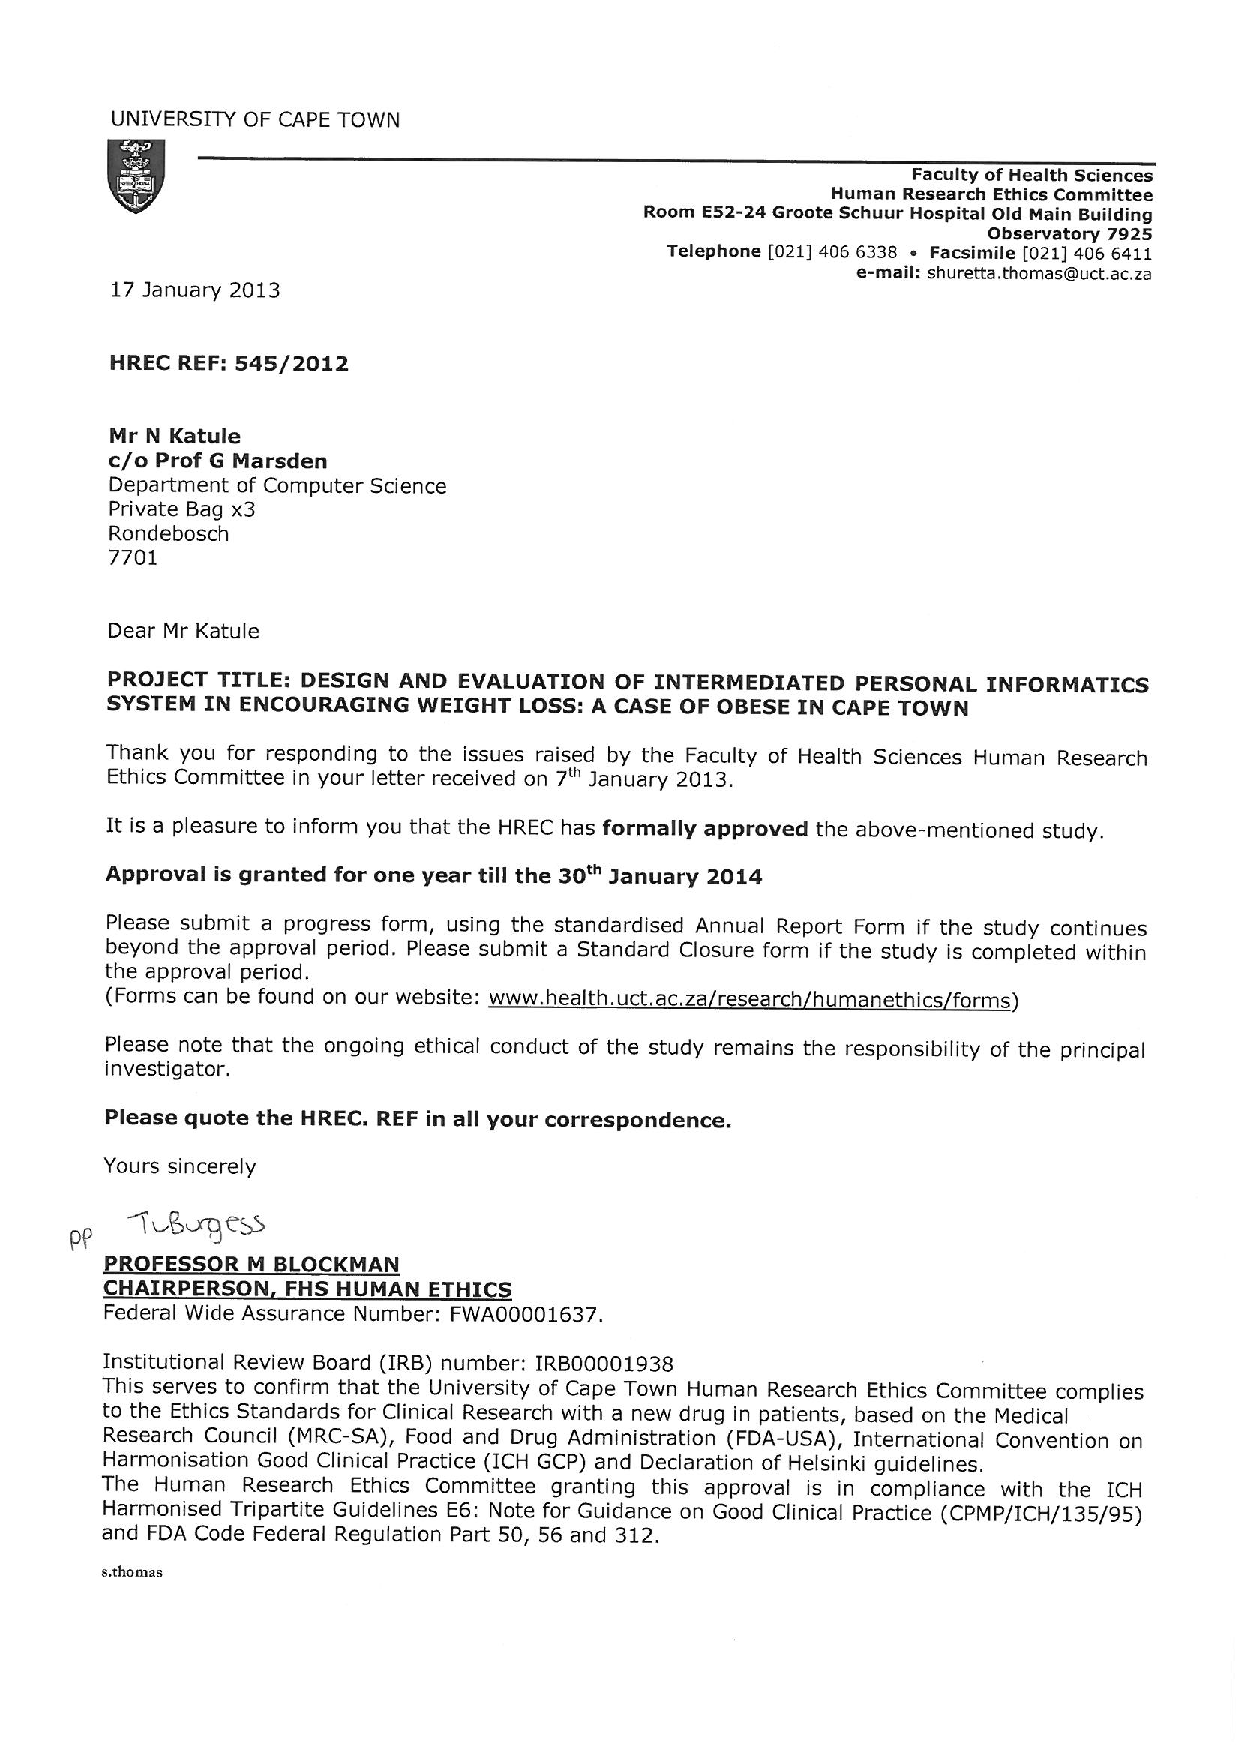
\includepdf[pages=-,pagecommand={},width=\textwidth,offset=90 -20]{Pdfs/fhsrec.pdf}

%\newcommand{\insertrep}[1]{%
%\hspace{-2.4cm}
%\fbox{\includegraphics[page=1,scale=0.8]{#1}}
%\includegraphics[page=1,scale=0.8]{#1}
%\includepdf[scale=0.75,pages=1,frame]{#1}
%}

%\subsection{Interesting Letter}
%\insertrep{Pdfs/baseline_ben.pdf}
%\begin{center}
%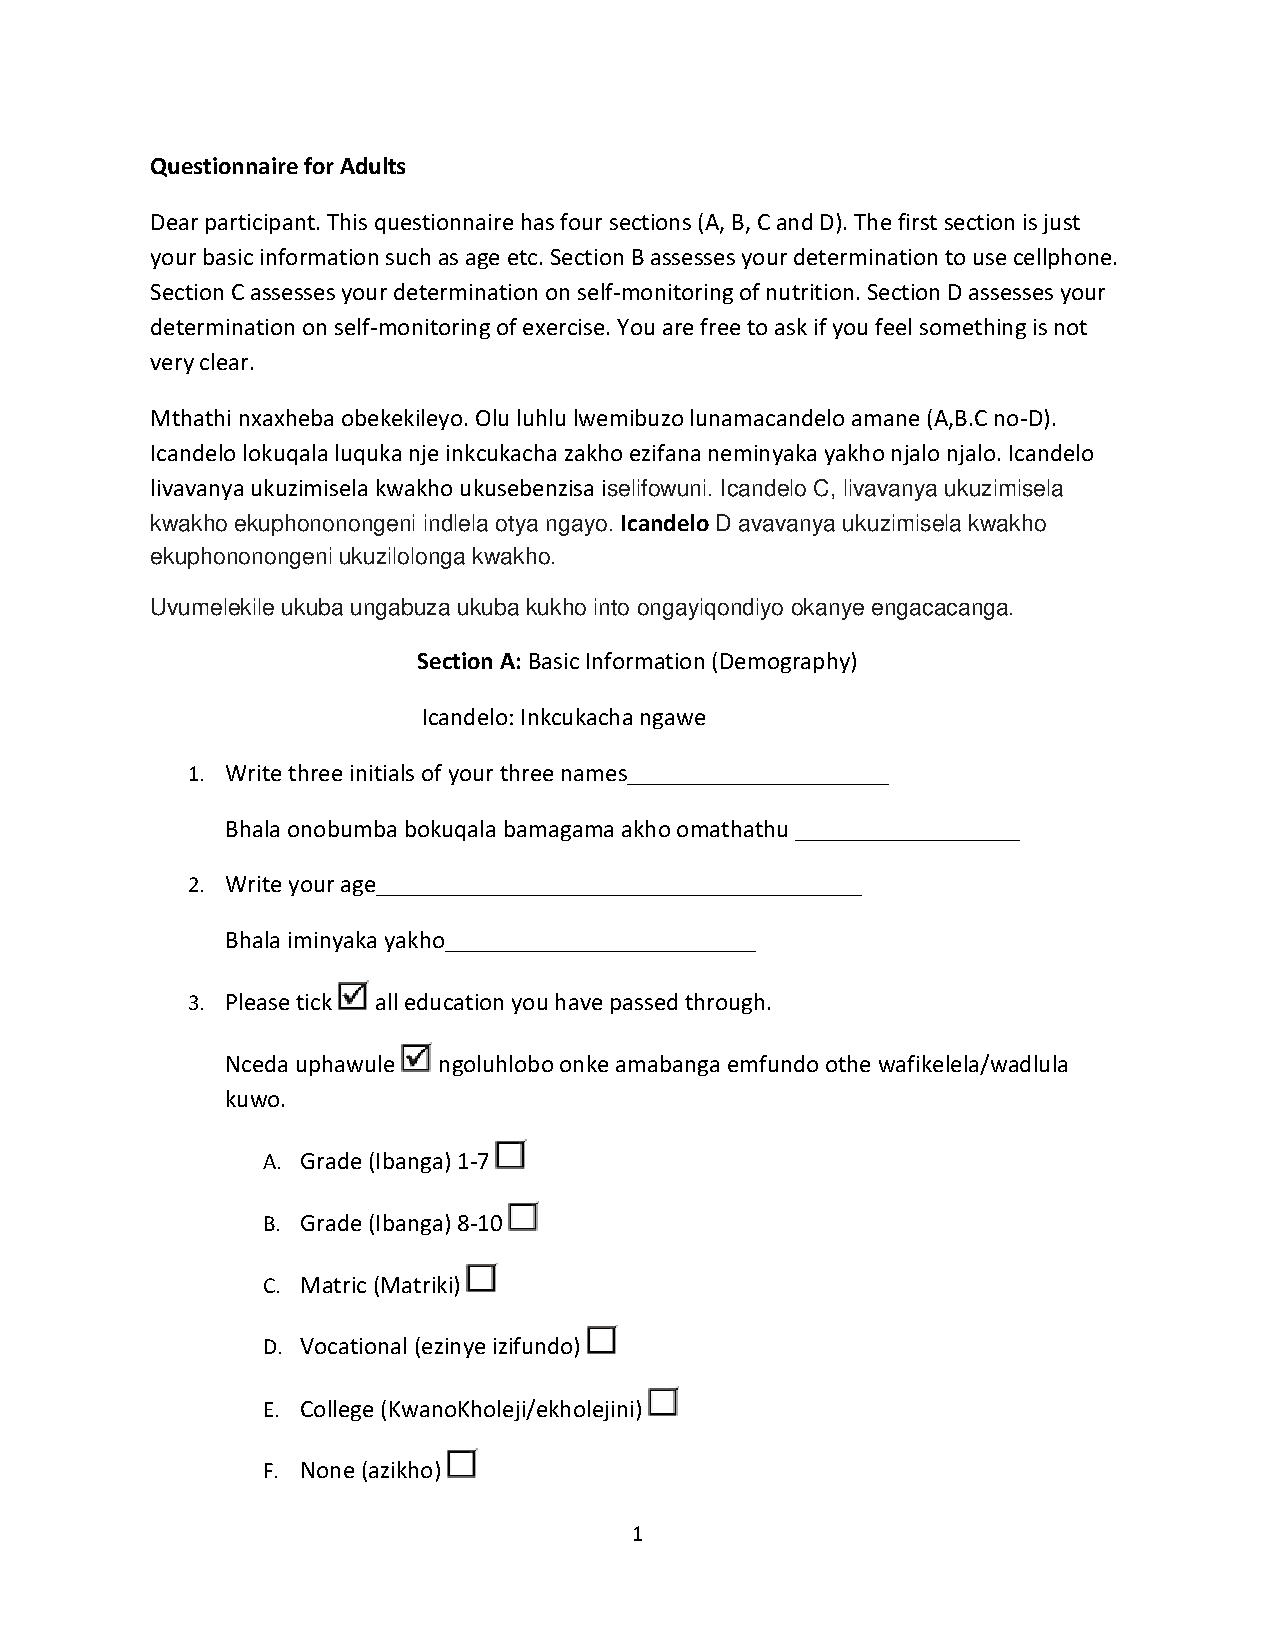
\includepdf[pagecommand={},scale=0.9]{Pdfs/baseline_ben.pdf} 
%\end{center}

%% Appendix A

\chapter{Appendix B. Ethics Approval -- Faculty of Science} % Main appendix title
\clearpage
\label{AppendixB} % For referencing this appendix elsewhere, use \ref{AppendixA}

\lhead{Appendix A. \emph{Ethics Approval -- Faculty of Science}} % This is for the header on each page - perhaps a shortened title

\includepdf[pages=-,pagecommand={},width=\textwidth,offset=90 0]{Pdfs/fsrec.pdf}

%\newcommand{\insertrep}[1]{%
%\hspace{-2.4cm}
%\fbox{\includegraphics[page=1,scale=0.8]{#1}}
%\includegraphics[page=1,scale=0.8]{#1}
%\includepdf[scale=0.75,pages=1,frame]{#1}
%}

%\subsection{Interesting Letter}
%\insertrep{Pdfs/baseline_ben.pdf}
%\begin{center}
%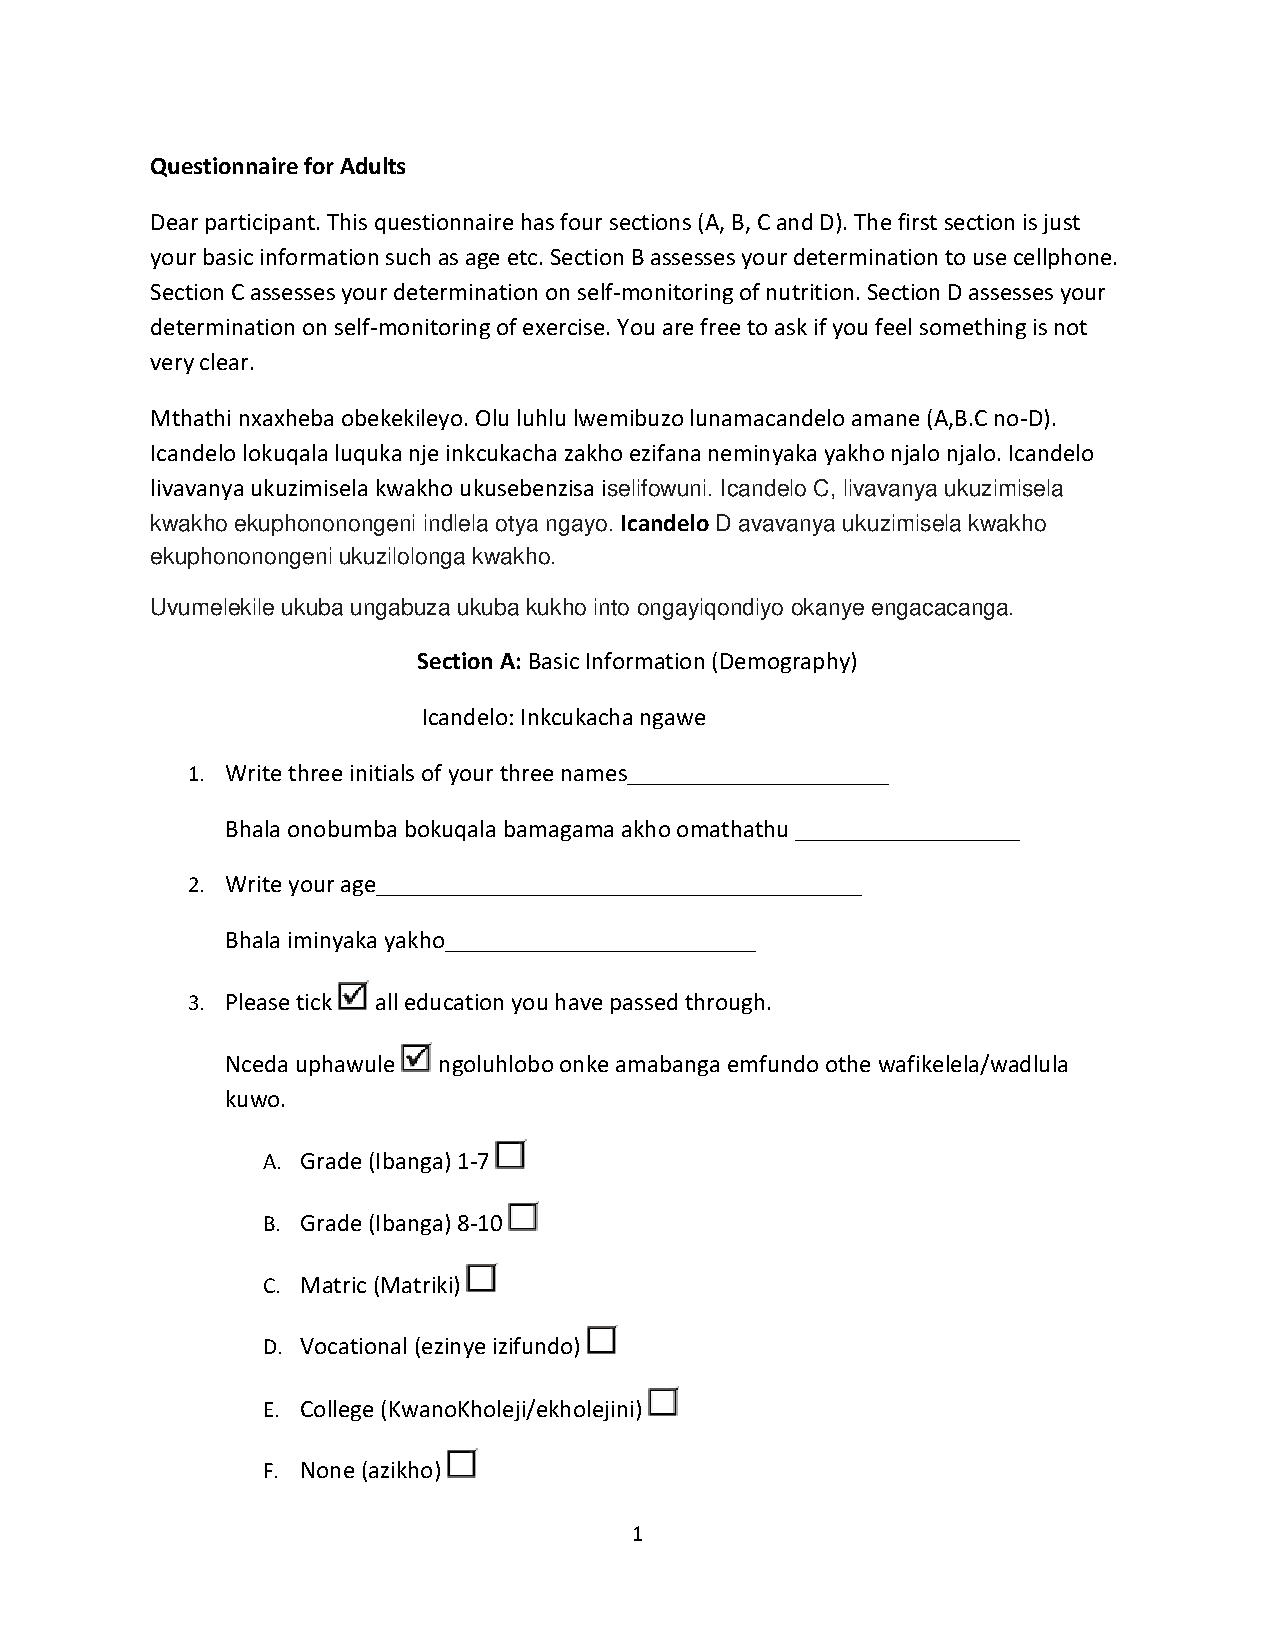
\includepdf[pagecommand={},scale=0.9]{Pdfs/baseline_ben.pdf} 
%\end{center}

%% Appendix A

\chapter{Appendix C. Baseline Questionnaires} % Main appendix title
\clearpage
\label{AppendixC} % For referencing this appendix elsewhere, use \ref{AppendixA}

\lhead{Appendix A. \emph{Baseline Questionnaires}} % This is for the header on each page - perhaps a shortened title
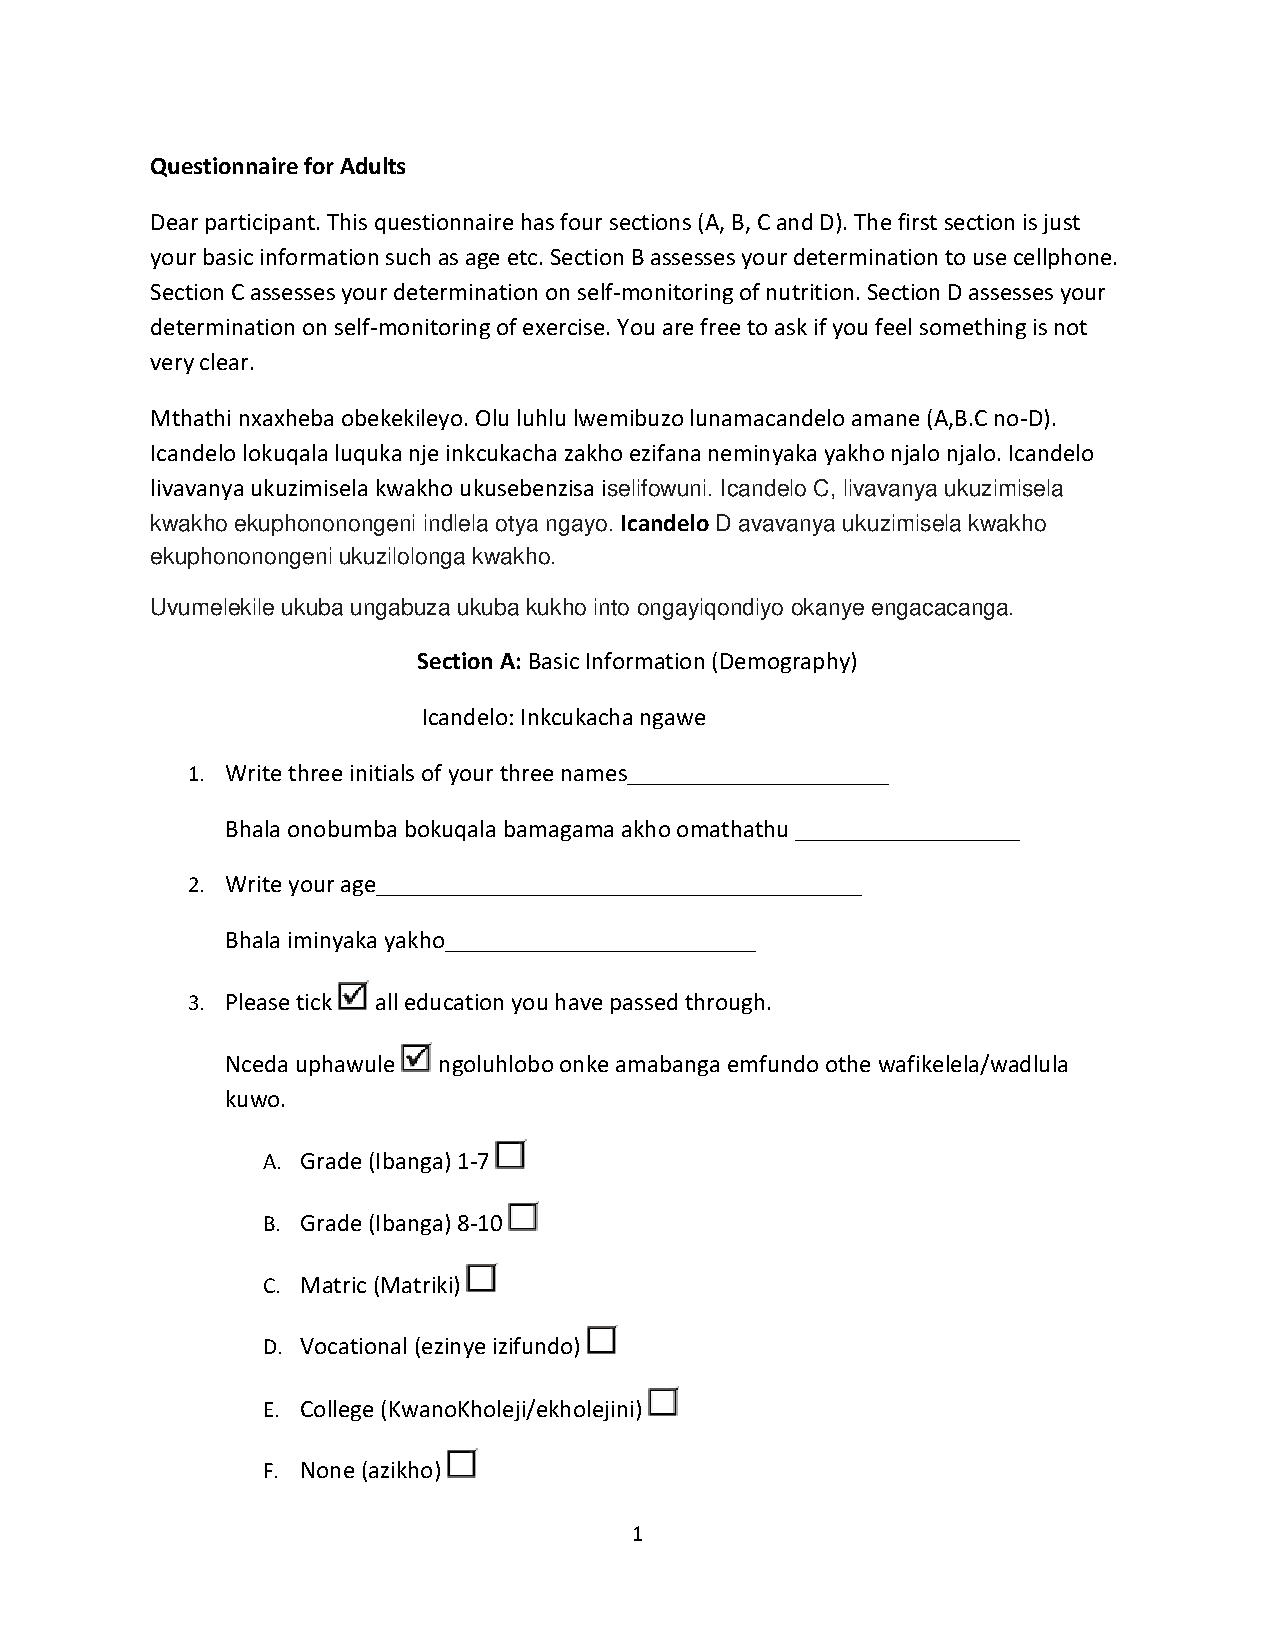
\includepdf[pages=-,frame,pagecommand={},width=\textwidth,offset=90 0]{Pdfs/baseline_ben.pdf}
\clearpage
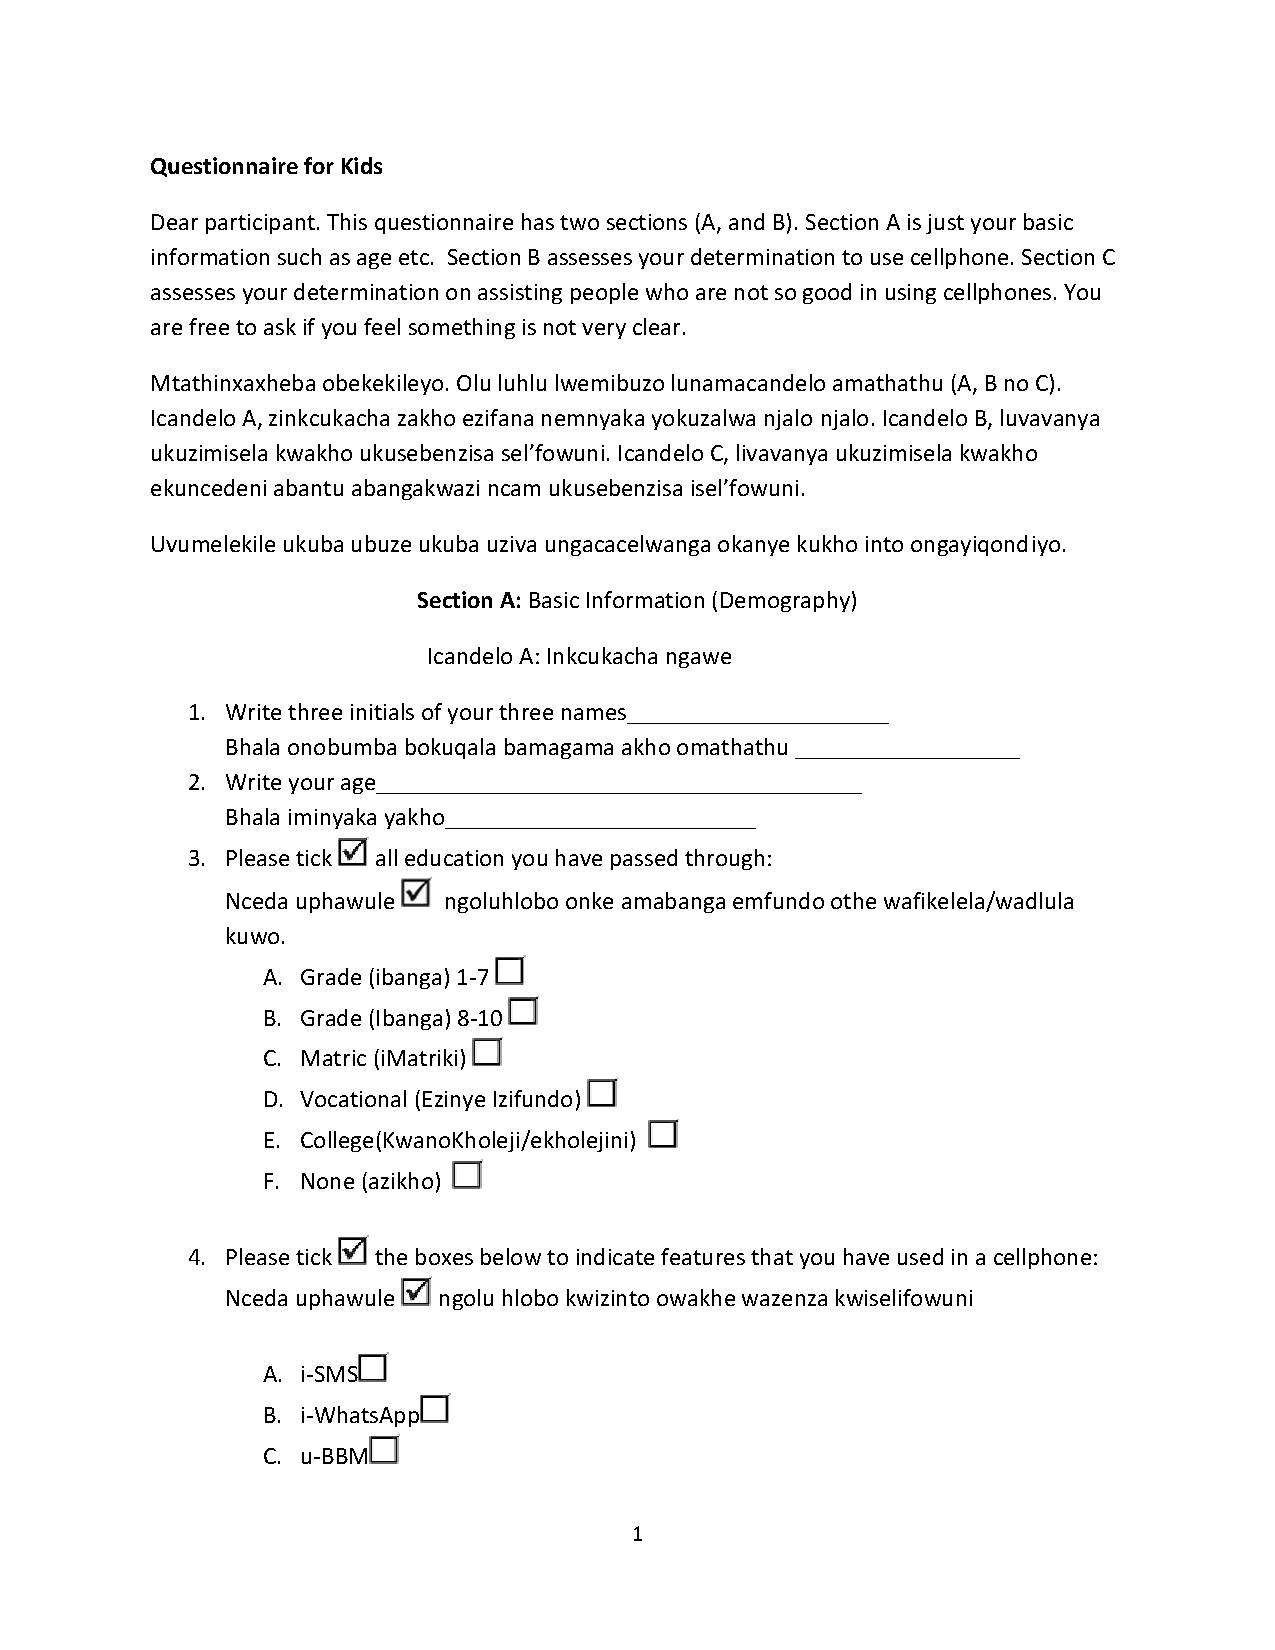
\includepdf[pages=-,frame,pagecommand={},width=\textwidth,offset=90 0]{Pdfs/baseline_interm.pdf}

%\newcommand{\insertrep}[1]{%
%\hspace{-2.4cm}
%\fbox{\includegraphics[page=1,scale=0.8]{#1}}
%\includegraphics[page=1,scale=0.8]{#1}
%\includepdf[scale=0.75,pages=1,frame]{#1}
%}

%\subsection{Interesting Letter}
%\insertrep{Pdfs/baseline_ben.pdf}
%\begin{center}
%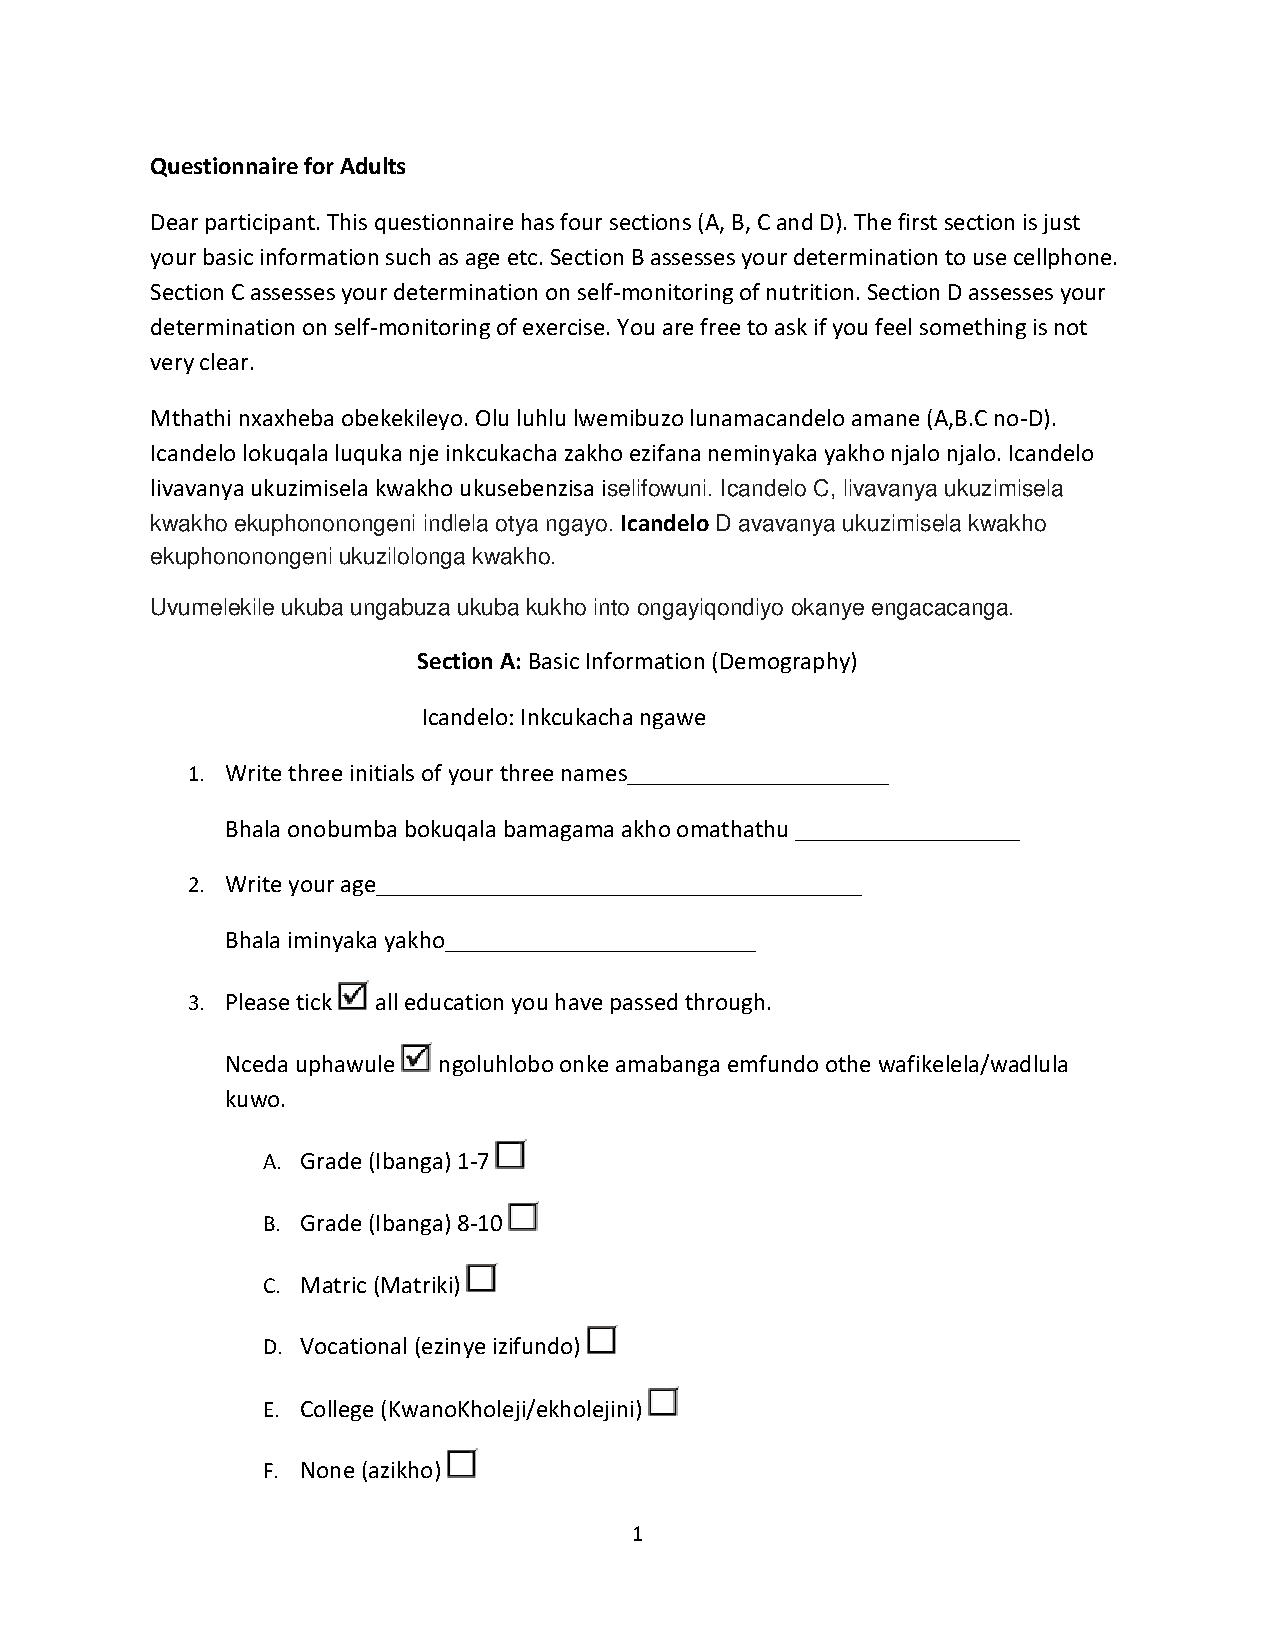
\includepdf[pagecommand={},scale=0.9]{Pdfs/baseline_ben.pdf} 
%\end{center}


\addtocontents{toc}{\vspace{2em}} % Add a gap in the Contents, for aesthetics

\backmatter

%----------------------------------------------------------------------------------------
%	BIBLIOGRAPHY
%----------------------------------------------------------------------------------------

\label{Bibliography}

\lhead{\emph{Bibliography}} % Change the page header to say "Bibliography"

\bibliographystyle{unsrtnat} % Use the "unsrtnat" BibTeX style for formatting the Bibliography

\bibliography{Bibliography} % The references (bibliography) information are stored in the file named "Bibliography.bib"

\end{document}  